\chapter{Salinidad Agrícola}
\section{Propiedades del agua y suelo}
Propiedades del agua y suelo relacionado con los procesos de salinización, recuperación y calidad química del agua de riego:

El agua contiene solutos, uso inadecuado de riego, los motivos del manejo ineficiente de riego 
problemas de salinización 
Se debe conocer el estado del Agua y suelo, origen de las sales, causas, identificar o caracterizar, diagnóstico (clasificación), análisis de las plantas (dónde afecta), prevención, corrección y adaptación. 
\begin{table}[h!]
    \centering
    \begin{tabular}{@{}ccc@{}}
    \toprule
    \multirow{3}{*}{\begin{tabular}[c]{@{}c@{}}Procesos de\\ ensalitramiento\end{tabular}} &
      Naturales &
       \\
     &
      \multirow{2}{*}{Inducidos} &
      Directo \\
     &
       &
      Indirecto \\ \midrule
    \multirow{2}{*}{\begin{tabular}[c]{@{}c@{}}Problemas de\\ Salinidad Agrícola\end{tabular}} &
      Salinización &
       \\
     &
      Sodificación &
       \\
    \multirow{2}{*}{Salinidad} &
      Agua &
       \\
     &
      Suelo &
       \\
    \multirow{3}{*}{Láminas} &
      De riego &
       \\
     &
      Requerimiento de lavado &
       \\
     &
      De lavado &
       \\
    \multirow{3}{*}{Zonas} &
      Áridas y semiáridas &
       \\
     &
      Áreas bajo riego &
      \begin{tabular}[c]{@{}c@{}}Distritos de riego\\ Unidades de riego\end{tabular} \\
     &
      Áreas de temporal &
       \\
    Distritos de Riego &
      \begin{tabular}[c]{@{}c@{}}Gravedad\\ bombeo\end{tabular} &
      \begin{tabular}[c]{@{}c@{}}RAS\\ PSI\end{tabular} \\
    Propiedades químicas &
      \begin{tabular}[c]{@{}c@{}}Solubles\\ intercambiables\end{tabular} &
       \\
    Cationes &
      \begin{tabular}[c]{@{}c@{}}Solubles\\ intercambiables\end{tabular} &
       \\
    \multirow{2}{*}{Caracterización} &
      Empírica &
       \\
     &
      Teórica &
       \\
    \multirow{2}{*}{\begin{tabular}[c]{@{}c@{}}Procesos de rehabilitación\\ de suelos afectados\end{tabular}} &
      Mejoramiento &
       \\
     &
      Recuperación &
       \\ \bottomrule
    \end{tabular}
    \caption{No confundir los conceptos}
    \label{tabs1}
    \end{table}
    La producción alimentaria es uno de los principales retos que tiene la humanidad y se prevé que la demanda mundial de alimentos se incrementará de manera importante para el año 2050, en un 70\% en lo general y casi el 100\% en los países en desarrollo. Este aumento aunado a una creciente competencia y demanda de los recursos naturales, ejercerá una presión sin precedentes en muchos sistemas de producción agrícola de todo el mundo. Dichos sistemas se consideran en peligro debido a que se les dé una especial atención y aplicar en su caso, medidas preventivas y correctivas específicas.

    Uno de los principales pilares de  la producción de alimentos a nivel mundial son las áreas irrigadas bajo aprovechamiento agrícola, cuyo incorporación al riego puede propiciar efectos negativos, entre los que destacan la salinización de los suelos (excesos de sales)
    
    \begin{definition}[Ensalitramiento]
        Es un proceso propiciado por el riego que consiste en la acumulación de sales en un suelo lo cual ocasiona que se rebasan las concentraciones normales que generalmente tienen; por lo tanto es de origen antropogénico
    \end{definition}
    Es importante recalcar que las sales minerales presentes en la solución del suelo disueltas como cationes y aniones, son imprescindibles para el crecimiento vegetal, pero cuando se acumulan y su concentración o tipos exceden ciertos límites, se puede afectar a los cultivos o al suelo en sí, impactando parcial o totalmente su productividad y por lo tanto, la de la superficie que se cultiva bajo riego.
    \begin{figure}[h!]
    \centering
      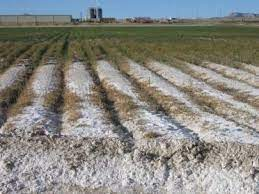
\includegraphics[width=0.5\textwidth]{s1.jpg}
      \caption{Suelo con problemas de ensalitramiento}
      \label{s1}
    \end{figure}
    Todos los problemas de salinidad agrícola son procesos antropogénicos que se presentan en áreas que se incorporan al riego, como una consecuencia implícita e inevitable pero no deseada, de un uso y manejo inadecuado del agua de riego.
    
    Es decir, el riego de los cultivos es un procesos que invariable e inevitablemente induce y ocasiona una acumulación de sales, ya sea en los suelos, en los mantos freáticos o en las aguas freáticas que se drenan y que descargan de las áreas bajo riego al mar o algún otro sitio, lo cual se debe a lo siguiente:
    \begin{itemize}
        \item A que todas las aguas de riego contienen solutos o sales en solución, en diferentes concentraciones y de varios tipos
        \item A que la finalidad teórica del riego, es suministrar al suelo una cantidad suficiente y adecuada de agua para que se almacene en él, y pueda ser aprovechada por los cultivos que se siembran para satisfacer sus demandas o requerimiento
        \item A que en teoría, el 99\% del agua de riego que se debe aplicar y almacenar en el suelo, se evapotranspira, y sólo una mínima parte de los solutos que contienen son aprovechados por los cultivos. Por tanto, la mayoría de ellos pueden irse acumulando en el suelo paulatina y progresivamente, su no se aplican las medidas necesarias para prevenirlo. Esto se conoce como ensalitramiento directo, primario o por arriba
        \item Por otro lado, el uso y manejo ineficiente del agua de riego ocasiona importantes pérdidas por infiltración profunda que puede propiciar la elevación de los mantos freáticos a niveles críticos s someros.
    \end{itemize}
    Su importancia radica en las extensas superficies en las que inciden, ya que los suelos afectados por las sales existen entre el 10\% y 20\% del total de la superficie cultivada bajo riego. México tiene 6.5 millones de hectáreas bajo riego y se considera como una nación joven en el contexto de la agricultura irrigada debido a la incorporación en 1926-1988 al riego en las áreas de los actuales distritos y unidades de riego.
    
    Existen 86 distritos de riego que ocupan una superficie aproximada de 3.3 millones de ha. Existen un poco más de 40,000 unidades de riego que ocupan una superficie aproximada de 3.2 millones de ha.
    
    \subsubsection{Agua}
    Es uno de los compuestos más antiguos del planeta; es el más abundante y el único que se encuentra en los tres estados al mismo tiempo, conformando a toda el planeta tierra.
    
    Se encuentran separados con un ángulo asimétrico de enlace de $104.54^{\circ}$
    
    Esto propicia que se forme una molécula dipolar con disposición irregular, que hace que las cargas de ambos átomos no se repartan uniformemente ni se contrarresten totalmente, se presentan cargas parciales positivas libres del lado de los hidrógenos y negativas libres del lado del oxígeno, originando los puentes de hidrógeno.
    
    El agua tiene propiedades físicas como la Cohesión, adhesión y capilaridad.
    
    \begin{definition}[Coehsión]
        Es la capacidad que tienen las moléculas que son iguales para atraerse y mantenerse unidas. En el caso de las del agua, los puentes de hidrógeno aportan una gran cohesión interna que las mantiene fuertemente unidas y atraídas entre sí, formando una estructura de tipo reticular o de geometría tetraédrica compacta que la convierte en un líquido casi incompresible.
    \end{definition}
    Esta propiedad es la que, en un momento lejano dado, fue la responsable de iniciar la retención de humedad dentro del suelo en la superficie específica de las partículas sólidas, como se detallará más adelante.
    
    También interviene de manera importante en la propiedad de capilaridad que se trata más adelante, y participa e influye directamente en la propiedad de retención de humedad en los espacios vacíos más pequeños del suelo, debido a que la cohesión propicia que cuando el agua pasa a través de ellos se quede almacenada en contra de las fuerzas de gravedad.
    \begin{definition}[Adhesión]
        Es la capacidad que tienen moléculas distintas para atraerse y mantenerse unidas, en el caso del agua, su enlace hidrógeno le otorga una alta propiedad de adhesión, que permite que cuando sus moléculas entran en contacto con otras moléculas o sustancias, se unan fuertemente a su superficie, manteniéndolas juntas o adheridas por fuerzas intermoleculares, siendo la razón por la que el agua moja.
    \end{definition}
    Esta propiedad es la que inicia la retención de humedad dentro del suelo en la superficie específicas de las partículas sólidas. También participa en el ensalitramiento directo.

También participa en la propiedad de capilaridad relacionada con los problemas de ensalitramiento indirecto de los suelos
  \begin{definition}[Capilaridad]
      La capilaridad se refiere a la tendencia del agua de poder ascender por un tubo estrecho en contra de la fuerza de gravedad, lo cual se debe a sus altars fuerzas de adhesión y cohesión.
  \end{definition}
Es decir, cuando se introduce un capilar en un recipiente con agua, ésta asciende como si trepase agarrándose por las paredes, pudiendo alcanzar un nivel superior al del recipiente hasta donde la presión que ejerce la columna de agua se equilibra con la presión capilar.

A esta propiedad se debe el ascenso de los mantos freáticos someros en áreas bajo riego, lo que propicia el ensalitramiento indirecto de los suelos o por abajo.

\subsection{Agua}
El agua es un compuesto con mucha reactividad y versatilidad química, debido principalmente a que su molécula es buena donadora de pares de electrones, favoreciendo lo siguiente:
\begin{itemize}
  \item Una constante dieléctrica muy alta, lo que la convierte en el solvente universal, por la gran cantidad de sustancias sobre las que puede actuar como disolvente.
  \item Una alta capacidad para reaccionar con compuestos que forman otros compuestos solubles.
  \item Un efecto catalítico que acelera casi todas las reacciones químicas.
  \item Es un buen reactivo químico, ya que puede funcionar como ácido o base, agente oxidante y agente reductor, entre otros aspectos.
\end{itemize}
\subsubsection{Constante Dieléctrica (Solubilización)}
Es la propiedad que tienen algunos compuestos con características polares para disolver o disociar iones de cargas opuestas, debido a la gran capacidad que tiene para formar puentes de hidrógeno con esas otras sustancias polares y iónicas.

En la solubilización participan dos sustancias, la primera es el solvente o disolvente como es el caso del agua, que es el medio en donde la segunda se separa, solubiliza o disuelve, formando lo que se conoce como iones en solución o solutos, (cationes para los de carga positiva y aniones para los de carga negativa).

Debido a su enlace de hidrógeno, el agua pura en forma líquida es un compuesto que presenta una de las más elevadas constantes dieléctricas.

Se considera la más importante en el tema de la salinidad agrícola, ya que por un lado define en gran parte la calidad química de las aguas de riego y por otro, es la que más participa tanto en los problemas de ensalitramiento de las aguas y de suelos, como en los procesos de lavado o recuperación de suelos ensalitrados
\begin{table}[h!]
  \centering
  \begin{tabular}{@{}cccc@{}}
  \toprule
  Sal & \begin{tabular}[c]{@{}c@{}}Solubilidad\\ (g/l)\end{tabular} & Sal & \begin{tabular}[c]{@{}c@{}}Solubilidad\\ (g/l)\end{tabular} \\ \midrule
  $MgSO_47H_2O$ & 710 & $KHCO_3$          & 252  \\
  $K_2CO_3$     & 526 & $Na_2SO_47H_2O$ &      \\
  $NaNO_3$      & 467 & $Na_2CO_3$       & 179  \\
  $CaCl_2$      & 300 & $Na_2SO_4$       & 161  \\
  $MgCl_2$      & 410 & $K_2SO_4$        & 100  \\
  $NaCl$        & 360 & $NaHCO_3$        & 87   \\
  $KCl$         & 340 & $CaSO_4$         & 2.4  \\
  $MgSO_4$      & 252 & $MgCO_3$         & 0.1  \\
  $Ca(HCO_3)_2$ & 262 & $CaCO_3$         & 0.01 \\ \bottomrule
  \end{tabular}
  \caption{Solubilidad de los principales solutos}
  \label{tabsa1}
\end{table}
\subsubsection{Conductividad eléctrica}
Se define como la facilidad con que el agua permite pasar la corriente eléctrica a través de sí misma, lo cual puede suceder a través de los solutos o sustancias de tipo electrolito disueltas o presentes en ella que conforman los aniones y cationes en solución. Su valor depende de la cantidad que contiene de solutos incrementándose a medida que esta aumenta, aunque no revela qué tipo de ellos que están presentes en el agua. 

La CE de un agua usualmente se expresa en unidades de milidecisiemens por metro (mdS/m) a diferencia de los suelos, en donde se utilizan decisiemens por metro (dS/m) por la mayor magnitud de los valores que puede alcanzar.

\subsubsection{Conductividad eléctrica}
La CE del agua de riego es uno de los parámetros más importantes para definir su calidad química, especialmente cuando es para fines de riego y, por tanto, permite evaluar el posible impacto negativo que pueda tener tanto en el ensalitramiento directo de los suelos que se rieguen como en los cultivos.

Es importante mencionar que, cuando se utiliza un agua para riego, los contenidos de sales que contendrá el suelo que se riega siempre serán de dos a cuatro veces mayores que los del agua, debido a los procesos evapotranspirativos. 

Otras aplicaciones adicionales e importantes del uso de los valores del parámetro CE, es que permite estimar y correlacionar a través de dos ecuaciones empíricas, y dentro de ciertos rangos de concentración, tanto el contenido total de solutos o sales disueltas en un agua de riego o en una solución de suelo expresado en unidades de peso, como los contenidos totales de aniones o de cationes en solución expresados en miliequivalentes por litro.

Ambas ecuaciones sirven para revisar y comprobar de manera general y aproximada si un análisis químico de agua o de suelo está bien hecho, específicamente para verificar los resultados de la determinación de los aniones y cationes.

Contenido total de sales disueltas en ppm o $mg/lt \approx 0.640 \times CE (mdS/m)$
(Su rango de validez es: 100 < CE (mdS/m) < 5,000)


Contenido de aniones o de cationes en meq/l en $meq/lt \approx 0.010 \times CE (mdS/m)$
(Su rango de validez es: 100 < CE (mdS/m) < 5,000)

\subsubsection{pH}
Es un índice que se usa para medir el grado de acidez o alcalinidad, que indica la concentración de iones hidrógeno presentes y se define como pH= log 1/[H+], variando sus valores entre el 0 y el 14. Cuanto mayor sea la concentración de iones de hidrógeno en el agua menor será el valor del pH y viceversa, por lo que el agua con un valor de pH inferior a 7.0 se considera ácida, si es superior a 7.0 se considera básica, y si es de 7.0 se considera neutra.

Este índice no influye de manera directa en los problemas de salinidad de las aguas o suelos, pero es muy útil como un indicador indirecto de la concentración que presentan de carbonatos y bicarbonatos de sodio, ya que a mayor contenido de ellos el pH se eleva, por lo que su valor está relacionado con la posible existencia de problemas de sodicidad en las aguas y en los suelos.

\subsubsection{Osmosis}
Es un fenómeno físico que consiste en el paso a través de una membrana semipermeable del solvente de una solución de menor concentración de sales a otra de mayor concentración, hasta el momento en que se equilibren éstas.

Es decir, es la tendencia de una solución a diluirse con otra con menor concentración cuando están separadas por una membrana semipermeable

Es un proceso que se presenta en las células de las raíces de las plantas, y consiste en que cuando en el suelo hay humedad aprovechable, el agua de la solución del suelo que es de baja concentración salina, pasa al interior de las raíces, que es una región de alta concentración, lo que sucede hasta que se igualan las concentraciones de ambas soluciones. Está relacionada con la salinidad de los suelos debido a que a mayor concentración de sales mayor presión osmótica (PO).

\subsubsection{Presión Osmótica}
Es la presión que se debe aplicar a una solución para detener el flujo neto de disolvente a través de una membrana semipermeable, manifestándose como un potencial osmótico o estado de energía de una solución debido a la presencia de sales disueltas dentro de ella, por lo que a mayor concentración mayor PO.

Existe una fórmula empírica para estimarla, utilizando el valor de la CE.
\begin{equation}
  PO \approx 0.36 \cdot CE \cdot 103
\end{equation}
\begin{notation}
  En donde:
  \begin{itemize}
    \item $PO$ = Presión osmótica en atm
    \item $CE \cdot 103$ = Conductividad eléctrica en dS/m.
  \end{itemize}
  Su rango de validez es $3 < CE\cdot 103 < 30$
\end{notation}
La PO participa de manera directa en la fórmula del Esfuerzo de Humedad del Suelo $(EHS = t + PO)$
\subsection{Suelos}
Principales propiedades físicas del suelo:
\begin{itemize}
  \item Componentes físicos
  \item Textura
  \item Estructura
  \item Porosidad
  \item Densidad aparente
  \item Superficie específica
\end{itemize}
\subsubsection{Componentes físicos sólidos minerales}
Los componentes sólidos del suelo provienen de la descomposición física de diferentes minerales, los cuáles se clasifican y denominan en tres tipos con base a su tamaño; y son las arcillas (R), los limos (L) y las arenas (A).
\begin{table}[h!]
  \centering
  \begin{tabular}{@{}cc@{}}
  \toprule
  \multicolumn{2}{c}{Clasificación de la ISSS} \\ \midrule
  \begin{tabular}[c]{@{}c@{}}Denominación\\ granulométrica\end{tabular} & \begin{tabular}[c]{@{}c@{}}Diámetros\\ aparentes\\ $\mu m$\end{tabular} \\
  Arcilla               & \textless{}2         \\
  Limo                  & 2-20                 \\
  Arena fina            & 20-200               \\
  Arena gruesa          & 200-2000             \\ \bottomrule
  \end{tabular}
  \caption{Clasificación de la Textura, según la ISSS}
  \label{tabsa2}
\end{table}
El contenido de cada una de estas tres partículas sólidas en el suelo se expresa en porcentaje, y los valores de los tres deben sumar 100\%, que en su conjunto determinan la textura y específicamente los tipos o grupos texturales de suelos. Los minerales de donde se originan las partículas sólidas del suelo a través de los procesos de intemperismo, principalmente físicos, son los que definen el tamaño de cada una de ellas y sus propiedades, de acuerdo a lo siguiente.

\textbf{Arcillas}. 

Están constituidas por silicatos de aluminio procedentes de la intemperización de rocas formadas por minerales tipo feldespato, piroxeno y micas, principalmente. Son minerales que poseen baja dureza, lo que facilita que con los procesos de intemperismo físico alcancen tamaños muy pequeños. Su estructura contiene tetraedros de sílice y octaedros de aluminio en diferentes proporciones y existen principalmente dos tipos de arcillas: las que tienen una proporción o relación 1:1 que están constituidas por una capa de silicatos y otra capa de aluminatos y las que son 2:1 que están compuestas por dos de silicatos y una de aluminatos. Hay varios grupos de arcillas, siendo los principales los de la caolinita, ilita, montmorillonita y vermiculita. Las capas de silicatos (tetraedros de $SiO_4$) son las que le otorgan a las arcillas las cargas negativas libres que forman parte sustancial del complejo de intercambio catiónico de los suelos CIC.

\textbf{Limos}

Provienen del intemperismo de los silicatos, aluminosilicatos y carbonatos de calcio principalmente, minerales que no son cohesivos y son de mediana dureza, lo que no les permite alcanzar medidas inferiores a 2 micras. Se forman generalmente de sedimentos transportados en suspensión por las corrientes de agua y por efecto del viento, los cuáles se depositan en el lecho de los ríos o sobre terrenos inundados.

\textbf{Arenas}

Proviene del intemperismo de las rocas consolidadas, compuesta principalmente de sílice en forma de cuarzo, mineral que posee una elevada dureza y, por esta razón, el tamaño de las partículas de arena es el más grande de las tres. Además, son el componente más inerte y de menor actividad en el suelo, ya que, entre otras razones, el cuarzo le otorga un bajo número de cargas electrostáticas, lo que ocasiona que tenga muy baja capacidad de intercambio de cationes (CIC).

\subsubsection{Textura}
La propiedad física más importante de los suelos es su textura, y especialmente el tipo y la cantidad de arcilla que contiene, ya que influye de manera significativa y determinante tanto en casi todas las demás propiedades físicas y químicas del suelo, como en las relaciones agua-suelo, de acuerdo con lo siguiente:
\begin{itemize}
  \item Propiedades físicas. Definen la porosidad, estructura, densidad aparente y superficie específica.
  \item Propiedades químicas. Influyen en el porcentaje total de sales, en la capacidad de intercambio de cationes y en el porcentaje de sodio intercambiable.
  \item Relaciones agua-suelo. Determinan la capacidad de retención de humedad, las constantes de humedad, la cantidad de humedad aprovechable, el movimiento de agua en el suelo y los valores de las láminas de riego y de lavado
\end{itemize}
La proporción de arcillas. limos y arenas define la clase textural a la que pertenece un suelo, que por la gran cantidad de permutaciones que se pueden dar de los tres componentes que son 970,200, el USDA los agrupó únicamente en 12 distintas clases de acuerdo al sistema de clasificación llamado Triángulo de Texturas que se ejemplifica numéricamente en el Cuadro siguiente. Es importante resaltar que la textura del suelo es una propiedad extremadamente difícil de modificar.

\subsubsection{Estructura}
La estructura del suelo se define, de manera general, como la disposición y
agrupación de las partículas minerales primarias o individuales de arena, limo y
arcilla presentes en unidades más grandes, conocidas como agregados o terrones.

Dependiendo de la forma geométrica y el tamaño en que se hallan dispuestos
dichos agregados, se le asigna un nombre o tipo de manera particular.
La estructura, junto con la porosidad, son las principales propiedades físicas de los
suelos arcillosos que se ven afectadas cuando se presentan excesos de sodio
intercambiable, ya que se provoca su defloculación.

\subsection{Porosidad del suelo}
Se refiere a los espacios vacíos que contiene; es decir, es el volumen de vacíos en
una unidad de volumen de suelo, los cuáles pueden estar ocupados por aire o por
solución del suelo. Su valor está en función principalmente de la textura, así como
de la estructura del mismo suelo, por lo que los suelos arcillosos tienen altos valores
$(\pm 60\%)$ y, por el contrario, los suelos arenosos contienen bajos valores (±40%).
Existen, de manera general, dos tipos de poros en los suelos, que son:
\begin{itemize}
  \item Los macroporos. Son los más grandes, en los cuales el agua puede circular con facilidad y drenarse hacia abajo por efecto de la gravedad, por lo que no se retiene en ellos; además, es en donde la aireación del suelo presenta una mayor actividad.
  \item Los microporos. Son los más pequeños y se les considera como poros capilares; en ellos el agua se retiene en contra de la gravedad debido a la propiedad de cohesión del agua y, además, es en donde ésta puede moverse capilarmente, ya sea lateralmente o hacia arriba.
\end{itemize}
Por tanto, la porosidad, y particularmente la cantidad de microporos están directamente relacionados con el problema de ensalitramiento indirecto de los suelos.

Además como ya se mencionó, puede ser afectada por la sodificación de un suelo y por los problemas de defloculación y compactación que se propician, ya que se reduce la cantidad de macroporos, se incrementa la de microporos y la capilaridad, y se reduce la permeabilidad y aireación.

\subsubsection{Densidad Aparente del suelo}
La densidad aparente de un suelo es la relación que existe entre la masa o peso de los sólidos y el volumen total que éstos ocupan, incluyendo el espacio poroso existente entre las partículas sólidas y se utiliza la siguiente expresión para calcularla:
\begin{equation}
  Da = \frac{P_{ss}}{V_{ts}} 
\end{equation}
\begin{notation}
  En donde:
  \begin{itemize}
    \item Da = Densidad aparente en $gr/cm^3$
    \item Pss = Peso del suelo seco, en gr.
    \item Vts = Volumen total del suelo = volumen de sólidos + volumen de vacíos.
  \end{itemize}
\end{notation}
El valor de la densidad aparente de los suelos bajo riego. puede variar entre 1.0 $g/cm^3$ en suelos muy arcillosos y bien estructurados, hasta alrededor de 1.5 g/cm3 en suelos migajón arcillo arenosos. Se utiliza para calcular la lámina pasiva de
\subsubsection{Superficie específica del suelo}
Es el área superficial externa total de las partículas sólidas contenidas en una cantidad unitaria de masa o de volumen de suelo, y a menor tamaño de las partículas mayor superficie específica en conjunto. Se relaciona directamente con la propiedad de retención de humedad del suelo, ya que funciona como área de contacto en donde se manifiesta la propiedad de adhesión de las moléculas de agua.

Existe un marcado contraste entre el área superficial de un suelo en donde dominan las partículas de arcilla que en el que lo hacen las de arena o limo. Para ejemplificarlo, se calculará el área específica de dos volúmenes iguales de suelo de 1,000 cm3 , incluyendo los poros, que se presentan en el Cuadro 1.5. Uno que contiene únicamente partículas de arcillas y otro sólo de limos, pero estableciendo dos supuestos totalmente irreales para simplificar los cálculos, que son que todas las partículas son cúbicas y todas son iguales
\begin{table}[h!]
\centering
\begin{tabular}{@{}ccccccccc@{}}
\toprule
Textura &
\begin{tabular}[c]{@{}c@{}}VTS\\ ($cm^3$)\end{tabular} &
\% P &
\begin{tabular}[c]{@{}c@{}}VS\\ ($cm^3$)\end{tabular} &
\begin{tabular}[c]{@{}c@{}}Lado de\\ 1 partic.\\ (mm)\end{tabular} &
\begin{tabular}[c]{@{}c@{}}Vol de\\ 1 partic.\\ ($mm^3$)\end{tabular} &
\begin{tabular}[c]{@{}c@{}}No. de\\ partic\end{tabular} &
\begin{tabular}[c]{@{}c@{}}AE de\\ 1 partic.\\ ($mm^2$)\end{tabular} &
\begin{tabular}[c]{@{}c@{}}AE total\\ ($m^2$)\end{tabular} \\ \midrule
Arcillas &
1000 &
60 &
400 &
0.001 &
$1\times 10^{-9}$ &
$4\times 10^{14}$ &
$6\times 10^{-6}$ &
2400 \\
Limos &
1000 &
40 &
600 &
0.01 &
$1.\times 10^{-6}$ &
$4\times 10^{14}$ &
$6\times 10^{-6}$ &
360 \\ \bottomrule
\end{tabular}
\caption{Superficie específica del suelo}
\label{tabsa3}
\end{table}
Esta propiedad está relacionada tanto con el problema de ensalitramiento indirecto de los suelos como con la cantidad total de agua que se requiere aplicar a un suelo afectado por sales para realizar su lavado.

\subsection{Principales propiedades químicas del suelo}
\begin{itemize}
\item Conductividad eléctrica
\item Porcentaje de sales
\item Complejo de intercambio catiónico
\item Capacidad de intercambio de cationes
\item Energía de adsorción de los cationes
\item Porciento de sodio intercambiable
\item pH
\end{itemize}
\begin{definition}[Solución del suelo]
Se refiere al conjunto formado por el agua y los solutos o cationes y aniones disueltos presentes en los espacios vacíos del suelo, en donde los principales aniones son cloruros ($Cl^{-1}$), sulfatos ($SO_4^{-2}$), carbonatos ($CO_3^{-2}$) y bicarbonatos ($HCO_3^{-1}$) y los cationes son sodio ($Na^{+1}$), calcio ($Ca^{+2}$), magnesio ($Mg^{+2}$) y potasio ($K^{+2}$), como se detallará posteriormente.
\end{definition}
\subsubsection{Conductividad eléctrica del suelo (CE)}
Es el parámetro más utilizado para estimar en forma cuantitativa la cantidad de sales que contiene un suelo, aunque no indica qué sales están presentes.

Usualmente se determina en un extracto de saturación obtenido de una pasta saturada de una muestra de suelo, lo cual se hace en laboratorio para simular las condiciones de la solución, y se expresa en dS/m por los valores que alcanza.

Se utiliza para clasificar si un suelo es o no salino, partiendo de lo que se menciona en el Manual 60 publicado por el USDA en 1954, en donde se define a un suelo salino como aquel cuya solución extraída de una pasta a saturación tiene un valor de CE de 4 dS/m o mayor

Además, es un parámetro que permite evaluar el efecto químico osmótico que pueden tener los excesos de sales en la solución del suelo, ya que participan directamente en el valor de la Presión Osmótica (PO) de dicha solución

La PO de la solución del suelo, a su vez, influye en la disponibilidad de agua almacenada en el suelo que puede ser aprovechada por los cultivos, ya que participa en la fórmula del Esfuerzo de Humedad del Suelo (EHS), que es:
\begin{equation}
EHS = T + PO
\end{equation}
\begin{notation}
En donde:
\begin{itemize}
\item $T =$ Tensión con la que está retenida la humedad por el suelo (en atm)
\item $PO =$ Presión osmótica (atm) $\approx 0.36 \cdot CE$ en dS/m
\item $CE =$ Conductividad Eléctrica en dS/m
\end{itemize}
\end{notation}
Es importante mencionar que la CE de la solución del suelo es dinámica, y como
consecuencia de los procesos evapotranspirativos, se va incrementando de manera
exponencial a medida que se reduce el contenido de humedad del suelo, concepto
que es importante considerar cuando se hable de manejo de cultivos en suelos con
problemas de sales

\subsection{Porcentaje de sales}
El valor de CE que se obtiene de un determinado suelo, es un excelente índice para determinar la concentración de sales en solución presentes en él, especialmente para clasificar el grado de afectación por salinidad que tiene, así como para utilizarlo como referencia para definir qué cultivos se pueden sembrar en suelos afectados.

Sin embargo, es un dato incompleto e insuficiente cuando se utiliza como base en un proceso de recuperación de suelos, debido a que, para un mismo valor de CE, suelos con diferentes texturas contienen distintas cantidades totales de sales.

Es decir, la CE determina la cantidad de sales presentes en una solución extraída de un suelo a saturación, lo que es una condición de humedad que varía fuertemente para cada tipo de textura de suelo, dependiendo de su porosidad. Por tanto, para un mismo valor de CE en iguales volúmenes de suelo, pero con diferentes texturas, a mayor porosidad mayor volumen de agua a saturación y, consecuentemente, un mayor peso o contenido total y real de sales y viceversa.

Por lo anterior, en el tema de salinidad agrícola se debe utilizar el índice de porcentaje de sales existentes en un suelo basado en el peso total de ellas, con la finalidad de contar con un valor más preciso del contenido total de sales que permita emitir un mejor diagnóstico del problema así como propuestas de solución más reales, especialmente de la lámina total de lavado.

Se presentan dos caminos distintos para estimarlo para tres suelos con diferentes texturas e iguales CE, con la finalidad de ejemplificar numéricamente las grandes diferencias que presentan dichos valores según sea el tipo textural del suelo.

El procedimiento seguido se basó en obtener el contenido de sales disueltas en los extractos de saturación de diferentes suelos para un mismo valor de CE de 10 dS/m, utilizando la fórmula $\sum ppm$ o $mg/lt \approx 0.640 \cdot CE (mdS/m)$, así como los valores representativos del contenido de humedad y densidad aparente para cada tipo de suelo, como sigue:
\subsubsection{Complejo de intercambio catiónico de un suelo}
La mayoría de las arcillas existentes en un suelo presentan en su superficie cargas negativas libres originadas por diferentes causas, las cuáles, de manera natural, se equilibran y contrarrestan con cationes provenientes de la solución del suelo, que pasan de ser solubles a intercambiables adsorbidos y viceversa, no pudiendo un catión ocupar las dos posiciones al mismo tiempo.

Las arcillas presentes, sus cargas negativas libres y los cationes intercambiables, son los que conforman el complejo de intercambio de un suelo.
\begin{figure}[h!]
\centering
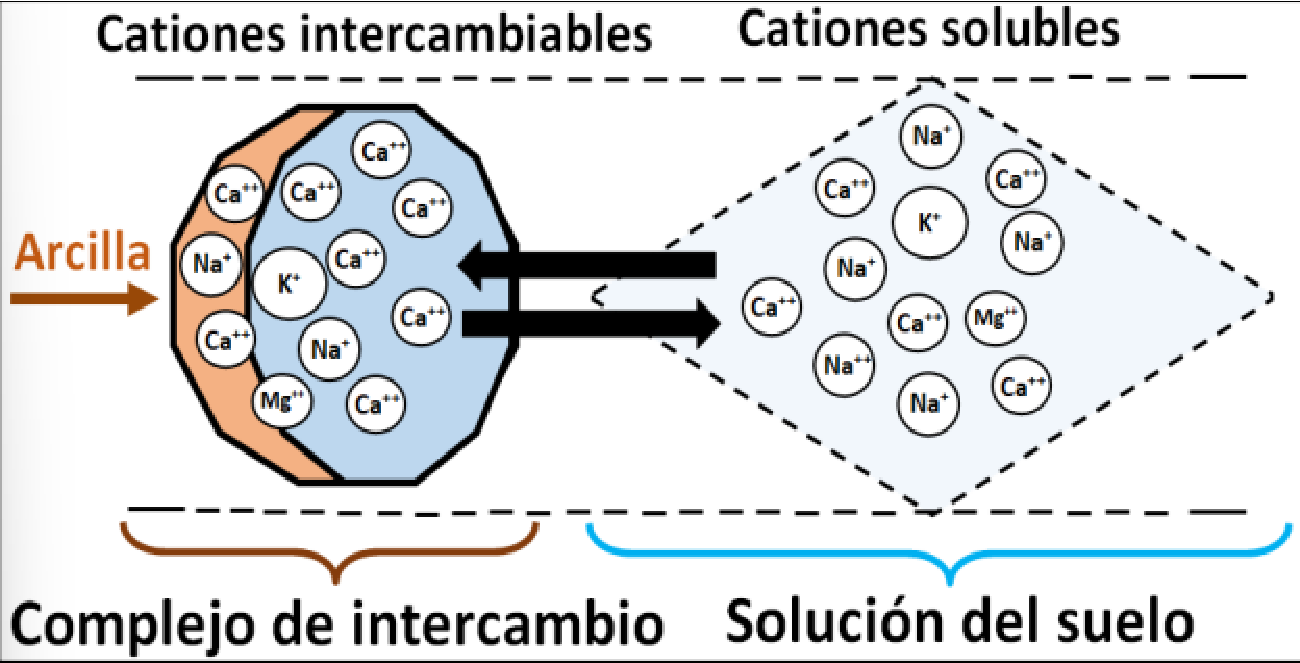
\includegraphics[width=0.5\textwidth]{s2.pdf}
\caption{Complejo de intercambio catiónico de un suelo}
\label{s2}
\end{figure}

\subsubsection{Capacidad de intercambio de cationes}
Es una propiedad que indica la cantidad de cargas electrostáticas negativas por unidad de peso que por diferentes causas tiene un suelo, que genera un proceso químico dinámico interno mediante el cual el complejo de intercambio puede retener algunos cationes que provienen de la solución del suelo, al tiempo que libera cantidades equivalentes de otros.

Este proceso, que se manifiesta de manera continua y reversible, se debe a la atracción electrostática que existe entre la superficie con cargas negativas libres de la arcilla y la carga positiva de los cationes solubles, generando una interacción que influye en el comportamiento químico y físico de los suelos.

La CIC se expresa en unidades de miliequivalentes por cada 100 gramos de suelo (meq/100 gr), cuyo valor depende de la cantidad y tipo de la arcilla que contiene, por ejemplo, las arcillas tipo 2:1 tienen mayor CIC que las 1:1 al tener dos capas de silicatos rodeando a los aluminatos.

Algunos valores de CIC de diferentes tipos de arcillas y texturas de suelo reportados por distintos autores, se muestran de manera orientativa en el cuadro siguiente:
\begin{table}[h!]
\centering
\begin{tabular}{@{}ccccc@{}}
\toprule
Tipo de arcilla &
Estructura &
\begin{tabular}[c]{@{}c@{}}CIC\\ (meq/100 gr)\end{tabular} &
\begin{tabular}[c]{@{}c@{}}Textura\\ del suelo\end{tabular} &
\begin{tabular}[c]{@{}c@{}}CIC\\ (meq/100 gr)\end{tabular} \\ \midrule
Vermiculita     & 2:1 & 100 - 150 & Arcilloso                                                  & \textgreater 30 \\
Montmorillonita & 2:1 & 70 - 120  & \begin{tabular}[c]{@{}c@{}}Franco\\ arcilloso\end{tabular} & 15 - 30         \\
Ilita           & 2:1 & 10 - 50   & Franco                                                     & 5 - 15          \\
Clorita         & 2:2 & 10 - 40   & \begin{tabular}[c]{@{}c@{}}Franco\\ Arenoso\end{tabular}   & 5 - 10          \\
Caolinita       & 1:1 & 3 - 15    & Arena                                                      & 1-5             \\ \bottomrule
\end{tabular}
\caption{Capacidad de intercambio de cationes}
\label{tabsa4}
\end{table}
\subsubsection{Energía de adsorción de los cationes}
La energía con la que los cationes presentes en la solución del suelo pueden ser primero atraídos y después retenidos o adsorbidos en el complejo de intercambio, se incrementa a medida que es mayor su valencia y para una misma carga, según sea su radio de hidratación. Por tanto, el orden decreciente de esta energía de los cationes más abundantes en los suelos indicado en la serie denominada liotrópica, es Ca > Mg > K > Na.

Consecuentemente, el calcio intercambiable es el que predomina en el complejo en la mayor parte de los suelos normales, debido a que su carga positiva es bivalente y tiene un radio de hidratación menor que el sodio, llegando a representar un 80% de los cationes adsorbidos, condición que propicia un efecto armonizante y floculante del suelo y, por tanto, una buena estructura.

Es decir, a pesar de que en la naturaleza el sodio ocupa el sexto lugar por su abundancia como componente en algunos minerales de la corteza terrestre (2.83\%), lo que propicia que sea el catión que predomina en la mayoría de las aguas de riego y por consiguiente en la solución del suelo, no sucede así en el complejo de intercambio, debido a que sólo tiene una carga positiva libre y un radio de hidratación mayor que el calcio.

Se destaca que los cationes intercambiables, al estar retenidos en el complejo, quedan protegidos contra los procesos de lixiviación, a diferencia de los que se encuentran en la solución del suelo, que pueden ser eliminados mediante lavados.

\subsection{Porciento de sodio intercambiable}
En un estudio de suelos ensalitrados es muy importante conocer el porcentaje que el sodio intercambiable representa en el complejo, debido a las repercusiones que en algunos casos se pueden ocasionar cuando su valor rebase ciertos límites y se alteren las proporciones que existían en relación con los otros cationes adsorbidos.

Esto puede suceder cuando en las aguas de riego o en las freáticas que asciendan por capilaridad se presentan altos contenidos de sodio soluble, lo que, consecuentemente, incrementa su concentración en el complejo de intercambio, pudiendo alcanzar niveles excesivos que no permitan que todas las cargas negativas de las arcillas se contrarresten y queden algunas libres, que es cuando aumentan las posibilidades de generar un real problema de sodificación de un suelo.

Cuando quedan cargas libres negativas sin compensar, se alteran y se rompe el equilibrio natural que existía en el complejo de intercambio, propiciando una repulsión entre las arcillas y una separación y dispersión de ellas; y por tanto, una desagregación o pérdida de la estructura del suelo conocida como defloculación, lo que combinado con la posibilidad de que las partículas de arcilla dispersas ocupen y tapen algunos microporos, se favorezca una cierta compactación del suelo.

Esta compactación puede ocasionar lo siguiente:
\begin{itemize}
\item Que se tengan que intensificar las labores de preparación y manejo del suelo, lo que incrementa los costos.
\item Que afecte la germinación y el crecimiento del sistema radicular de los cultivos
\item Que se reduzca el intercambio gaseoso entre la atmósfera y el suelo y, por tanto, se limite la capacidad de oxigenación en la zona radicular.
\item Que sea más lenta la infiltración del agua de riego y su movilidad dentro de él, pudiéndose crear condiciones de exceso de humedad que a su vez puede propiciar el ahogamiento de los cultivos o enfermedades fungosas.
\item Que se afecte el desarrollo de los cultivos y su productividad.
\item Que se incrementen los problemas de ensalitramiento indirecto.
\end{itemize}
La importancia de este tema motivó que, en los años cuarenta del siglo XX, en el
Manual 60 de USA se desarrollara el concepto de Porcentaje de Sodio
Intercambiable (PSI), cuya fórmula es la siguiente:
\begin{equation}
PSI = SI \cdot 100/CIC
\end{equation}
\begin{notation}
En donde:
\begin{itemize}
\item PSI = Porcentaje de Sodio Intercambiable, en \%.
\item  SI = Sodio Intercambiable, en meq/100 gr suelo.
\item  CIC = Capacidad de intercambio de cationes, en meq/100 gr suelo.
\end{itemize}
\end{notation}
En el Manual 60 los autores proponen que un valor mayor al 15\% de sodio intercambiable define y clasifica a un suelo como sódico, ya que consideran que es el límite crítico a partir del cual se altera el equilibrio existente en el complejo de intercambio y se presente un cambio brusco en las propiedades de éste, pudiendo afectar desfavorablemente su productividad, aunque es importante resaltar que en el mismo Manual 60 se menciona la dificultad que los autores tuvieron para elegir dicho límite de PSI.

Es decir, los autores consideraron que el valor de 15\% era un límite tentativo y arbitrario de separación entre los suelos no sódicos y los sódicos, debido a que no contaban con la suficiente experiencia o datos que justificara un cambio a éste límite, además de que las metodologías que se utilizaban en esa época para estimar los efectos dañinos del sodio intercambiable al suelo estaban en proceso de superación

Sin embargo, a pesar de los inconvenientes que los mismos autores del Manual 60 señalan que tiene el límite de PSI de 15\%, a la fecha se continúa utilizando en muchos lugares del mundo de manera incorrecta debido a que no se cuenta con el conocimiento preciso tanto de las condiciones reales en que suceden los problemas de sodificación en un suelo, como de los efectos específicos que se pueden presentar y cuando pueden suceder en diferentes escenarios

Por tanto, se debe ser muy cuidadoso con el uso del límite de 15 de PSI de un suelo, ya que para que realmente se presenten problemas de sodicidad o sodificación que no dependen únicamente del PSI, el autor considera que tienen que concurrir varias condiciones y situaciones específicas, algunas de ellas de manera simultánea, las cuáles son

\begin{itemize}
\item Que el agua de riego o del manto freático tenga altos contenidos de sodio soluble ocasionando que predomine en la solución del suelo.
\item Que el suelo tenga contenidos de arcillas mayores a 40\% y por lo tanto valores de CIC mayores a 20 o 25 meq/100 gr de suelo.
\item Que el suelo tenga contenidos de arena menores a 40\%.
\item Que la concentración de sales en el suelo sea baja.
\item Que el sodio intercambiable alcance niveles excesivos en el complejo de intercambio y propicie que queden cargas negativas libres de las arcillas.
\item Que se manifieste de manera importante una de floculación y compactación del suelo.
\item Que el suelo presente valores mayores de pH de 8.5
\end{itemize}
Por lo anterior, el autor considera que se requiere profundizar más sobre este tema, para evitar utilizar de manera imprecisa o incorrecta el valor de 15\% de SI del Manual 60, con la finalidad de no cometer errores al asignar el término de sódico a un suelo, por tener un valor mayor a dicho límite.

Esto es, aunque un suelo con una baja CIC; por tener bajo contenido de arcillas y alto de arenas, puede presentar valores de PSI mucho mayores a 15, y aunque suceda defloculación en los agregados y una cierta compactación del suelo, la presencia de las arenas minimiza, contrarresta y encubre los efectos y consecuencias que se presentan cuando hay una verdadera sodificación.

En cambio, un suelo con altos contenidos de arcilla, una elevada capacidad de intercambio de cationes y bajos contenidos de arena, puede presentar síntomas de sodicidad con valores menores de 15\% de sodio intercambiable.

\subsubsection{pH del suelo}
Los valores que presenta el pH de la mayoría de las aguas y suelos bajo riego son mayores a 7, debido a que las sales que se pueden combinar entre los principales aniones y cationes que predominan en ellos son predominantemente del tipo básico y neutro

La importancia del pH en el tema de la salinidad agrícola radica en que es un excelente indicador de los problemas de sodicidad de los suelos, ya que la abundancia con la que se presentan los carbonatos y bicarbonatos de sodio en los suelos sódicos propicia que su valor generalmente sea mayor a 8, y que inclusive rebase el valor de 8.8 cuando el problema es muy fuerte

\subsection{Relaciones agua-suelo}
\begin{itemize}
\item Capacidad de retención de humedad
\item Contenido de humedad
\item Constantes de humedad
\item Clases de agua
\item Relación de las constantes de humedad con los procesos de lavado
\item Diferentes movimientos de agua
\end{itemize}
\subsubsection{Capacidad de retención de humedad}
Se refiere a la cantidad de agua que puede almacenar o retener un suelo en sus espacios porosos en contra de la fuerza de gravedad, lo que sucede debido a la atracción que existe entre las moléculas del agua y el suelo, conocidas como fuerzas de tensión de humedad o potencial mátrico.

Esta retención de humedad de los suelos se presenta únicamente en sus microporos y se desarrolla en tres etapas y en tres diferentes capas de agua que se forman. Participan dos propiedades del agua; que son la adhesión y la cohesión y dos del suelo, definidas por la textura del suelo, que son la superficie específica total de las partículas y la cantidad de microporos presentes. Las tres etapas son:
\begin{enumerate}
\item Primera etapa inicial estática y primera capa permanente de agua adherida a la superficie específica:

Es la que se inició en algún momento dado muy lejano, cuando algunas moléculas de agua llegaron y pentraron en el suelo, y formaron una primera capa adherida a la superficie específica de las partículas sólidas presentes en él, la cual es permanente debido a que las fuerzas de tensión con la que está retenida el agua son altísimas, pudiendo alcanzar valores de más de 10,000 atmósferas.

Esto implica que ningún suelo agrícola puede secarse completamente de manera natural, ya que ello sólo podría suceder bajo condiciones de laboratorio a temperaturas mayores a $105^{\circ}C$. La cantidad de moléculas de agua adheridas en esta primera capa dependen directamente del total de superficie específica del suelo


\item Segunda etapa inicial estática y segundas capas de agua retenidas en el suelo por cohesión casi permanentemente.

A esa primera capa de agua adherida a las partículas del suelo, también hace tiempo por cohesión, se unió una segunda capa de agua y después se unió otra a la segunda, y así sucesivamente hasta llegar a una enésima capa que sería el límite con la tercera etapa.

La cantidad de capas de agua cohesionadas dependen directamente de la cantidad de microporos existentes en el suelo, en donde las fuerzas de tensión de las capas se van reduciendo a medida que aumenta su distancia de la superficie específica, teniendo la última capa un valor de referencia de 30 a 15 atmósferas.
\item Tercera etapa activa o dinámica y terceras capas de agua retenidas por cohesión.

Se presenta exclusivamente después de un riego a través de la formación de
capas cohesionadas de agua subsecuentes a la última capa de la segunda
etapa.

La cantidad de capas de agua cohesionadas en esta tercera etapa también
dependen directamente de la cantidad de microporos en el suelo.

En ésta última etapa, las fuerzas de tensión también se van reduciendo en cada
capa de agua de 15 atmósferas, hasta que se hace prácticamente nula cuando
el suelo alcanza su máxima capacidad de retención de humedad, que
corresponde a una tensión de referencia de 0.3 atmósferas.
\end{enumerate}
\begin{figure}[h!]
\centering
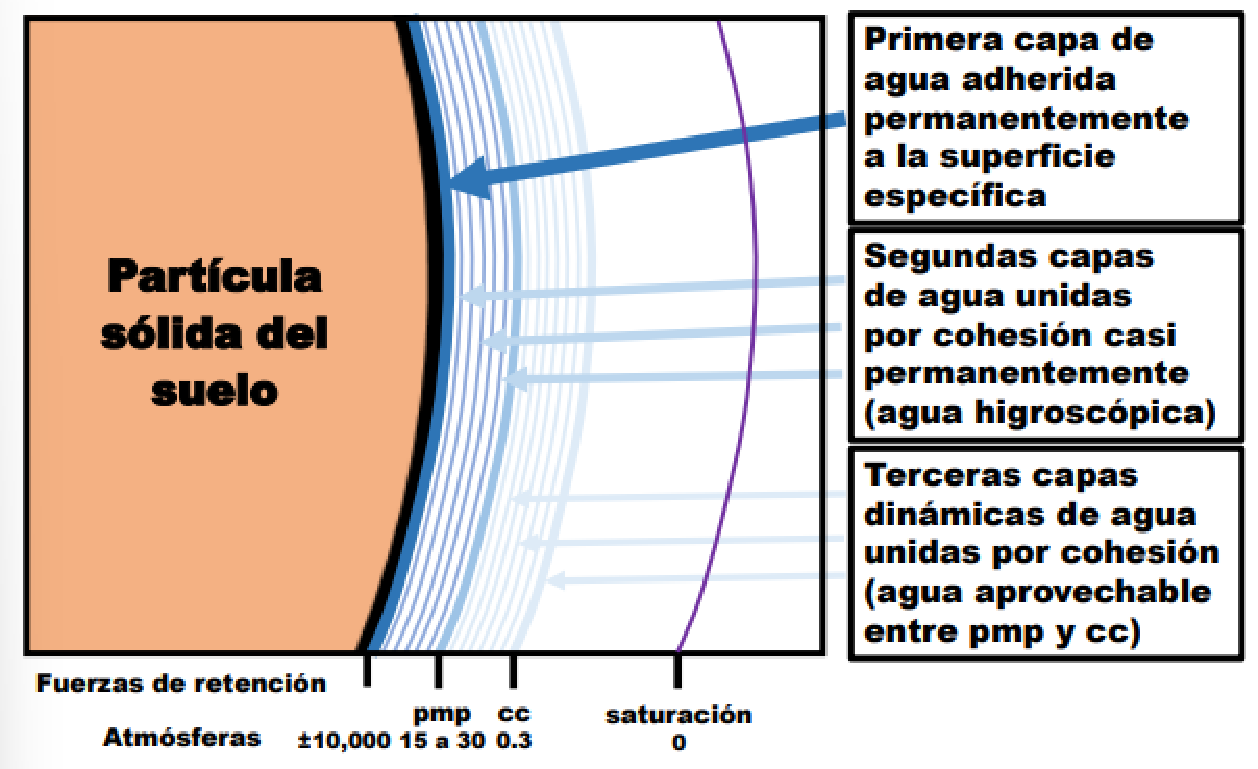
\includegraphics[width=0.5\textwidth]{s3.pdf}
\caption{Capacidad de retención de humedad}
\label{s3}
\end{figure}
\begin{figure}[h!]
\centering
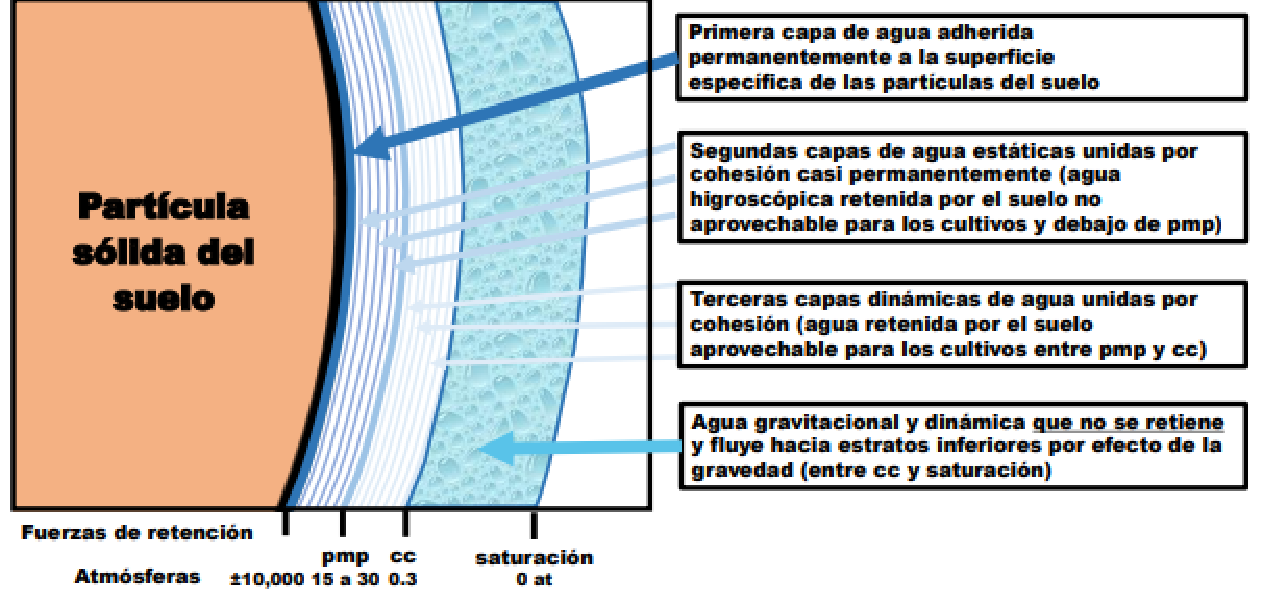
\includegraphics[width=0.5\textwidth]{s4.pdf}
\caption{Retención de la humedad en el suelo, en las subláminas de lavadp}
\label{s4}
\end{figure}
\begin{figure}[h!]
\centering
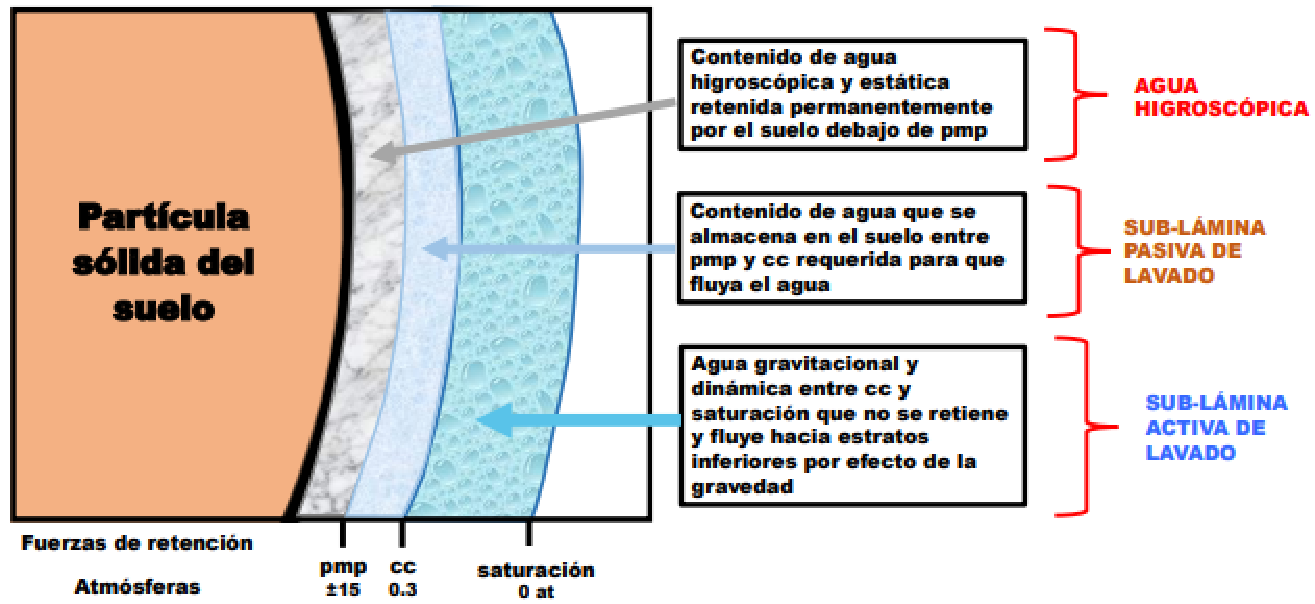
\includegraphics[width=0.5\textwidth]{s5.pdf}
\caption{Tipos de agua, en las subláminas de lavado.}
\label{s5}
\end{figure}
Antes de aplicar una lámina de riego a un suelo, su contenido de humedad en teoría será igual o un poco mayor al que corresponde al principio de la tercera capa.

La relación que existe entre la capacidad de retención de humedad y los problemas de salinidad agrícola, consiste en que influye tanto en el contenido total de sales de un suelo como en la determinación del valor de las diferentes láminas de lavado de los suelos afectados, como se explicará más adelante.
\begin{equation}
LR = (cc-pmp) \times  Da \times prof 
\end{equation}
Esta agua es retenida o inmovilizada temporalmente en los microporos o poros capilares de un cierto espesor de suelo, hasta que se inician los procesos de evapotranspiración.

\subsubsection{Contenido de humedad}
Es la cantidad de agua que contiene un suelo en un momento dado, y su valor depende tanto de las entradas de agua y de sus salidas, como del tipo de textura del suelo; por lo que es muy variable en el tiempo y en el espacio.

Se puede expresar en diferentes formas, siendo la más utilizada la de humedad gravimétrica (Ps), la cual se define como la relación entre el peso del agua existente en una determinada masa de suelo y el peso de las partículas sólidas, expresada en porcentaje, y generalmente referida a 100 gr de masa de suelo.
\begin{equation}
PS = \frac{(Psh - Pss) \cdot 100}{P_{ss}} = \frac{(Pa * 100)}{P_{ss}}
\end{equation}
\begin{notation}
En donde:
\begin{itemize}
\item Ps = Contenido de humedad, \%.
\item Pss = Peso del suelo seco, gr.
\item Psh = Peso del suelo húmedo, gr.
\item Pa = Peso del agua contenida, gr.
\end{itemize}
\end{notation}
Las diferentes condiciones o factores que propician distintos contenidos de humedad de un suelo bajo riego, han sido estudiadas, revisadas y analizadas por varios investigadores desde un punto de vista agronómico, las cuáles fueron relacionadas con el diseño y la aplicación de riego y con los requerimientos de agua de los cultivos, lo que permitió establecer las constantes de humedad.

Es decir, dado que los contenidos de humedad que puede presentar un suelo bajo riego, varían dependiendo de las entradas y salidas que tengan de agua, las constantes de humedad se establecieron como límites basados en la disponibilidad de agua para los cultivos y los tipos de agua existentes en él.

Las tres constantes son saturación, capacidad de campo y punto de marchitez permanente, y varían de manera importante para cada tipo de textura del suelo, pudiéndose estimar cada una de ellas en dos tipos de unidades, en porcentajes y en valores de tensión de humedad o fuerzas de retención (atmósferas).

\subsubsection{Saturación}
Se dice que un cierto espesor de suelo está saturado cuando todos sus poros están llenos de agua, lo que puede suceder después de un riego o de una lluvia fuerte y solo por un corto instante, siendo el valor de la tensión de humedad en el suelo en ese momento de cero atmósferas.

La relación que existe entre la capacidad de retención de humedad y los problemas de salinidad agrícola, consiste en que influye tanto en el contenido total de sales de un suelo como en la determinación del valor de las diferentes láminas de lavado de los suelos afectados, como se explicará más adelante.

\subsubsection{Capacidad de campo (cc)}
Es cuando un suelo está en su máxima capacidad de retención de agua en
contra de la fuerza de gravedad, siendo una condición también instantánea
debido a que dura minutos. Otras formas de expresarla son:
\begin{itemize}
\item Es el contenido de humedad que permanece en el suelo entre 24 y 48 horas después de la aplicación de un riego o de una lluvia fuerte, dependiendo de la textura del suelo, cuando cesa prácticamente el movimiento descendente del agua por efecto de la gravedad.
\item Es cuando se encuentra al 100\% de humedad aprovechable, que es el límite superior del agua del suelo a partir del cual pueden extraerla los cultivos.
\item Es cuando aproximadamente 50\% de los espacios vacíos del suelo se encuentran llenos de agua.
\item Es el contenido de humedad que tiene el suelo cuando las fuerzas de tensión con las que el agua se encuentra retenida están a ±0.3 atmósferas.
\end{itemize}
Aunque para la capacidad de campo el valor de tensión de referencia es de 0.3 atmósferas, sus valores puntuales dependen del tipo de textura de suelo y casi no varían, de tal manera que en los suelos muy arcillosos se aproximan a 0.25 y en los francos a 0.35.

Se resalta que para que el agua que se aplique como riego pueda empezar a fluir verticalmente por efecto de la gravedad dentro del suelo, principalmente en los macroporos, el contenido de humedad debe encontrarse entre capacidad de campo y saturación.
\subsection{Punto de marchitamiento permanente (pmp)}
Como ya se mencionó, el contenido de humedad de un suelo bajo riego es muy dinámico, ya que después de la aplicación de un riego, y a partir de que el contenido de humedad llega a capacidad de campo en un cierto espesor de suelo, éste empieza a disminuir, como consecuencia de la evaporación directa del suelo y por la extracción de agua por los cultivos.

En el momento en que las raíces del cultivo ya no pueden extraer agua retenida en el suelo debido a que las fuerzas de retención del mismo son mayores a las que puede desarrollar para absorberla, se llega al límite de contenido de humedad que se conoce como punto de marchitamiento permanente.

Otras formas de expresarlo son:
\begin{itemize}
\item Punto en el que una planta de girasol con 4 o 5 hojas se marchita y no recupera su turgencia por más que se riegue.
\item Cuando en el suelo se presenta un 0\% de humedad aprovechable para los cultivos, es decir, es el límite inferior de contenido de humedad aprovechable.
\item Cuando aproximadamente 25\% de los espacios vacíos del suelo contienen agua.
\item Contenido de humedad que tiene el suelo cuando las fuerzas de tensión con las que el agua se encuentra retenida están a 15 atmósferas.
\end{itemize}
Aunque el valor de 15 atmósferas es el que está fijado como límite de referencia para el pmp, su rango de variación es muy amplio debido a que lo definen las características fisiológicas del cultivo de acuerdo con su sensibilidad o tolerancia a condiciones de estrés hídrico en el suelo, pudiendo ser de entre 12 y 15 para los cultivos susceptibles, y de 15 a 20 o más para los resistentes.

Relación de las constantes de humedad con los procesos de lavado:

Las constantes de humedad, son propiedades directamente relacionadas con la lámina total de agua y las láminas parciales que se tienen que aplicar en los procesos de recuperación de suelos ensalitrados, ya que a diferencia de los objetivos que tiene la aplicación de un riego, que es llevar a capacidad de campo un cierto espesor de suelo, la finalidad de los lavados es crear condiciones de humedad que permitan el flujo vertical del agua con sales disueltas por gravedad hacia estratos inferiores, lo que solamente puede suceder cuando la humedad se encuentra entre el punto de capacidad de campo y el de saturación.

Así, la cantidad total de agua que se requiere aplicar para el lavado de un suelo afectado por sales está compuesta por dos láminas parciales, que son la de riego o pasiva de lavado (LPL) que no participa en la eliminación de sales y la Lámina activa de lavado (LAL) que es la que realmente lixivia la sales
\subsubsection{Clases de agua}
Hay tres clases o categorías de agua en el suelo limitadas por las constantes de humedad, las cuáles fueron definidas con base a su posibilidad de ser aprovechadas por los cultivos
\begin{itemize} 
\item Agua gravitacional o no aprovechable. Es la porción del agua de riego que se aplica al suelo que se drena libremente del primer estrato de suelo hacia los inferiores por acción de la fuerza de gravedad, lo que sucede principalmente en los macroporos del suelo. Dicha agua no es aprovechable para las plantas, y es la que se encuentra entre los límites de humedad de saturación y de capacidad de campo, con valores de tensiones de referencia de 0 hasta 0.3 de atmósferas.
\item Agua aprovechable o retenida disponible o capilar. Es aquella parte del agua aplicada que se retiene en los microporos capilares del suelo en contra de la gravedad y que puede ser aprovechada por las plantas Esta agua se encuentra entre los límites de humedad de capacidad de campo y punto de marchitamiento permanente, con tensiones de 0.3 hasta 15 atmósferas como referencia.
\item Agua higroscópica retenida no aprovechable. Es la parte del agua aplicada que se almacena en los microporos del suelo que no puede ser aprovechada por las plantas, debido a que las fuerzas de tensión con las que está retenida son mayores a las que pueden desarrollar las plantas para extraerla. Esta agua se encuentra abajo del límite de humedad de punto de marchitamiento permanente, con tensiones de 15 o 35 hasta 10,000 atmósferas como referencia.
\end{itemize}

\subsection{Diferentes movimientos de agua}
La principal propiedad y tipos de movimiento de agua del suelo son:
\begin{itemize}
\item Permeabilidad. Es la propiedad que tiene el suelo de facilitar o permitir la transmisión o circulación del agua y del aire dentro de él.
\item Percolación. En riego se refiere a la penetración vertical del agua en un suelo o paso a través de él en los espacios porosos, conocido también como filtración.
\item Infiltración. Es la velocidad con que penetra el agua de la superficie hacia el interior del suelo. Es de gran importancia para el especialista en irrigación, ya que participa en el diseño de los diferentes sistemas de riego. Se expresada en mm/hora. Hay dos tipos de infiltración, una que se presenta al inicio de la aplicación del riego cuando el contenido de humedad del suelo es bajo hasta que llega a la saturación, por lo que va disminuyendo hasta volverse constante, que es cuando se alcanza la segunda infiltración conocida como básica.
\item Conductividad hidráulica. Es la velocidad con la que se mueve el agua dentro del suelo en condiciones de saturación (mantos freáticos) y se utiliza para diseñar drenaje parcelario
\end{itemize}
\subsection{Calidad química de las aguas de riego}
La calidad química del agua para riego se refiere principalmente a como es su composición de elementos minerales solubilizados. Se determina utilizando los resultados que se obtienen de un análisis en laboratorio o campo de una muestra de agua, los cuales permiten conocer la composición y concentración de los constituyentes químicos que contiene en solución, para con ellos aplicar las diferentes normas y estándares de calidad química que existen al respecto.

Su finalidad principal, es evaluar, tanto las bondades que pueda tener al utilizarla para riego, como los riesgos potenciales de producir efectos dañinos al suelo, a los cultivos, a los sistemas de riego o a los animales y personas que consumen los cultivos que se irrigan, destacando los siguientes posibles impactos.
\begin{itemize}
  \item A corto plazo influye en el tipo, la producción y la calidad del cultivo.
  \item A largo plazo algunas aguas pueden perjudicar el suelo a través de su salinización o sodificación, hasta hacerlo totalmente improductivo para la agricultura.
\end{itemize}
Lo anterior indica que, si la calidad del agua de riego no es adecuada, independientemente de que se tengan condiciones y prácticas agronómicas óptimas en un proceso de producción, dicha agua no permitirá que se obtengan buenos resultados.

En el caso contrario de un agua de riego con una calidad química adecuada, ésta condición no es garantía de que no se tengan consecuencias negativas, específicamente de problemas de drenaje interno y de ensalitramiento indirecto de los suelos, como se explicará más adelante.

Por lo anterior, se tratará de manera detallada lo relacionado con la calidad química del agua de riego, enfocada y aplicada básicamente a problemas de salinización, sodificación, fitotoxicidad y otros que se pueden presentar como consecuencia de su aplicación para riego de los cultivos en los suelos.

Sólo se mencionará de manera introductoria, lo del Criterio Agronómico de la Calidad del Agua de Riego, tema que se tratará detalladamente más adelante.

Desde hace más de 50 años, varios autores introdujeron el concepto de Calidad Agronómica del agua de riego, la cual toma en cuenta, además de su calidad química, las interacciones agua-suelo-planta y los principales factores que participan en un proceso productivo, como son el suelo por regar, el cultivo, el método de riego que se utilice y el manejo integral que se realice, principalmente

Esto se debió a que si la información de la calidad química es de mucha utilidad para evaluar su potencial para fines de riego, no es suficiente para realizar predicciones más certeras que permitan determinar los problemas específicos que se pueden causar, por ejemplo, la salinización indirecta en el caso de los sistemas de riego por gravedad o la sodificación en algunos suelos, ya que la manifestación de estos problemas no se debe exclusivamente a la composición química del agua, sino que además intervienen los factores agronómicos mencionados que también participan en los procesos productivos.

Este término el suscrito lo retomó y complementó con la finalidad de buscar y proponer alternativas para el aprovechamiento de aguas de riego que presentan algún problema de calidad química, llamándolo CRITERIO AGRONÓMICO DE LA CALIDAD DEL AGUA DE RIEGO.

Las principales determinaciones químicas que generalmente se realizan en un agua de riego, son de la concentración de sales solubles que se miden a través de la CE eléctrica, del contenido de aniones en solución (cloruros, sulfatos, carbonatos y bicarbonatos), del contenido de cationes en solución (sodio, calcio, magnesio y potasio) y del pH. Sólo en casos especiales se determinan otros aniones y cationes.

Los resultados de estas determinaciones químicas se utilizan en los principales índices o parámetros que han desarrollado diferentes investigadores para definir la calidad química del agua para riego, los cuales el autor agrupó con base en qué es lo que pueden afectar o qué tipo de problema puede causar cuando ser presentan resultados desfavorables, obteniendo cuatro criterios de agrupación, que son:
\subsubsection{Calidad química del agua de riego}
Se resalta que la gran mayoría de los técnicos y personas utilizan en general solamente los índices de CE, RAS y pH, pero, para el caso de los estudios y trabajos más detallados relacionados con salinidad agrícola, se recomienda aplicar todos los índices propuestos, con la finalidad de, por un lado, aprovechar la información que se obtiene del análisis químico y, por el otro, para complementar, reforzar y confirmar los diagnósticos positivos o negativos que se realicen con los índices sobre la calidad química del agua de riego.

Para contar con información más completa, especialmente deben utilizarse en el tema del efecto probable de los excesos de sodio y sus posibles consecuencias de sodificación, por ser un problema mucho más complicado de estudiar, comprender, clasificar y aplicar que el de concentración de sales solubles, debido a que participan factores y componentes mucho más complejos.
\subsubsection{Índice para clasificar la concentración de sales solubles y el posible efecto del tipo de sales}
Expresa la concentración de sales del agua de riego referida a una temperatura de $25^{\circ} C$ y sus unidades son mdS/m o micromhos/cm. Es el parámetro más utilizado para determinar la concentración de sales por la simplicidad, rapidez y precisión con la que se puede determinar su valor, ya sea en el laboratorio o en el campo, además de que tiene. Algunos valores de CE de referencia de varios tipos de aguas son:

Los límites y rangos que han utilizado distintos investigadores para definir las diferentes clases de concentración de sales de las aguas de riego basados en la CE, se han determinado tomando en cuenta las características particulares que tienen las aguas de su país.

Destaca una de las más conocidas, que es la del Laboratorio de Salinidad de los Estados Unidos de América (Manual 60, 1954), cuyos límites de valores de CE se aplicaron con base en la información existente en esa época de las aguas utilizadas para riego en los Estados Unidos, y relacionándolas con posibles problemas de salinidad o sodicidad de los suelos.

Sin embargo, se considera que es una clasificación excesivamente estricta, ya que la primera clase con base a la CE, es de 100 hasta 250 micromhos o mdS/m, lo que definitivamente no se aplica a la gran mayoría de las aguas de riego que tienen otros países
\begin{table}[h!]
  \centering
  \begin{tabular}{@{}cccc@{}}
  \toprule
  Clase &
    \begin{tabular}[c]{@{}c@{}}CE\\ (micromhos/cm)\end{tabular} &
    \begin{tabular}[c]{@{}c@{}}CE\\ (micromhos/cm)\end{tabular} &
    \begin{tabular}[c]{@{}c@{}}Peligro de\\ salinidad\end{tabular} \\ \midrule
  1 & 100- 250           & 0.1 - 0.25        & Bajo     \\
  2 & 250 - 750          & 0.25 - 0.75       & Medio    \\
  3 & 750 - 2,250        & 0.75 - 2.25       & Alto     \\
  4 & \textgreater 2,250 & \textgreater 2.25 & Muy alto \\ \bottomrule
  \end{tabular}
  \caption{Conductividad Eléctrica (CE)}
  \label{tabsa5}
\end{table}
Como se observa, el valor de CE de 250 micromhos/cm que se utilizó en ese momento para delimitar la primera clase de agua de riego con base en su concentración de sales solubles, no es congruente con las que se presentan en otros países del mundo ya que, si se aplicara dicho límite, solamente un mínimo porcentaje de ellas estaría en primera clase, lo que definitivamente no es real.

Es decir, aunque esta clasificación fue una buena propuesta para EUA, la realidad de las aguas de riego en muchos países, ha propiciado que diferentes investigadores propongan otros límites del contenido de sales

Riesgo de salinización directa según la clase:
\begin{enumerate}
  \item Mínimo
  \item Bajo a mediano (vigilar RL pero no es necesario cuando se riega por gravedad)
  \item Mediano a alto (indispensable RL, especialmente en riego localizado)
  \item Alto a muy alto (muy indispensable aunque impráctica la aplicación de la RL, uso preferentemente con goteo o hidroponía)
  \item Extremadamente alto (uso prohibitivo en cualquier sistema de riego por gravedad, solo utilizable con hidroponia hasta ciertos límites)
\end{enumerate}
Se usa para estimar suma de cationes o de aniones, PO y sales totales disueltas

Este índice fue propuesto, con la finalidad de estimar el peligro potencial de las sales solubles presentes en el agua de riego que más influyen en la disponibilidad de agua para las plantas, tomando en cuenta que cuando se reduce el contenido de humedad en el suelo, se puede presentar una precipitación de las sales menos solubles (Doneen, 1959).

Por tanto, en su planteamiento excluye de la salinidad total los carbonatos y sulfatos de calcio y magnesio que se pueden precipitar por ser poco solubles, ya que dejarían de participar en la elevación de la presión osmótica, quedando en solución las sales más solubles, que son los cloruros y los sulfatos, los cuales pueden aumentar considerablemente la presión osmótica. Para estimar la SE plantean cuatro posibilidades, de acuerdo con la proporción que existe de los cationes calcio y magnesio y de los aniones carbonatos, bicarbonatos y sulfatos, que se presentan en las siguientes fórmulas.

\subsubsection{Salinidad efectiva (SE)}
\begin{itemize}
  \item Si $Ca > (CO_3 + HCO_3 + SO_4)$, en meq/lt: $SE = \sum Cationes - (CO_3 + HCO_3 + SO_4)$
  \item Si $Ca < (CO_3 + HCO_3 + SO_4)$, en meq/lt: $SE = \sum Cationes - Ca$
  \item Si $Ca < (CO_3 + HCO_3)$, pero $(Ca + Mg) > (CO_3 + HCO_3)$,en meq/lt: $SE = \sum Cationes - (CO_3 +HCO_3)$
  \item Si $(Ca + Mg) < (CO_3 + HCO_3)$, en meq/lt: SE = $\sum Cationes - (Ca + Mg)$
\end{itemize}
\begin{table}[h!]
  \centering
  \begin{tabular}{@{}cccc@{}}
    \hline
  Iones & Valencia & \begin{tabular}[c]{@{}c@{}}Peso molecular\\ (mg/m mol)\end{tabular} & \begin{tabular}[c]{@{}c@{}}Peso\\ equivalente\\ (mg/meq)\end{tabular} \\ \hline
  \multicolumn{4}{c}{Cationes}      \\
  Sodio        & +1 & 22.99 & 22.99 \\
  Calcio       & +2 & 40.08 & 20.04 \\
  Magnesio     & +2 & 24.32 & 12.16 \\
  Potasio      & +1 & 39.10 & 39.10 \\
  \multicolumn{4}{c}{Aniones}       \\
  Cloruros     & -1 & 35.46 & 35.46 \\
  Sulfatos     & -2 & 96.06 & 48.03 \\
  Carbonatos   & -2 & 60.01 & 30.01 \\
  Bicarbonatos & -1 & 61.02 & 61.02 \\ \hline
  \end{tabular}
  \caption{Peso molecular y peso equivalente de los solutos con mayor frecuencia en las aguas de riego}
  \label{tabs6}
\end{table}
\begin{table}[h!]
  \centering
  \begin{tabular}{@{}cc@{}}
  \toprule
  Sal    & \begin{tabular}[c]{@{}c@{}}Miliequivalentes\\ por litro\end{tabular} \\ \midrule
  NaCl & 24                                                                   \\
  $CaCl_2$  & 32                                                                   \\
  KCl    & 24                                                                   \\
  $MgCl_2$  & 32                                                                   \\
  $Na_2SO_4$ & 36                                                                   \\ \bottomrule
  \end{tabular}
  \caption{Cantidad necesaria de miliequivalentes de diferentes sales para producir una solución con una presión osmótica equivalente a una atmósfera}
  \label{tabs7}
\end{table}
El sodio es el catión que más daño puede ocasionar a un suelo, ya que su presencia en exceso en el complejo de intercambio altera el equilibrio catiónico y puede originar una desagregación, defloculación y pérdida de la estructura del suelo, propiciando una compactación con todas sus consecuencias.

\subsection{Norma combinada del Manual 60 (1954)}
Es del Laboratorio de Salinidad de EU (Manual 60, 1954), y es de las más conocidas a nivel mundial. Está basada en la Relación de Adsorción de sodio (RAS) en donde proponen un diagrama con 16 clases para diferentes valores de CE y RAS.

El RAS expresa la concentración relativa del sodio respecto al calcio y magnesio solubles presentes en un agua de riego, con la finalidad de estimar el efecto potencial directo del contenido de sodio que puede saturar el complejo de intercambio, el cual se calcula utilizando la siguiente fórmula en meq/l:
\begin{equation}
  RAS = \frac{Na}{\sqrt{\frac{Ca +}Mg{2}}} 
\end{equation}
En general, ha existido una confusión en el uso de dicho norma, especialmente el diagrama que combina valores de CE con rangos de RAS, ya que estos últimos no son lineales y por tanto fijos y varían para cada rango de CE. Es decir, hay que combinarlos para asignar a qué clase de agua de riego corresponde de las 16 que tiene, y el RAS va aumentando a medida que se incrementa el contenido de solutos

% TODO: GRAFICAAAAAAAAAAA

Es decir, una mayoría de los usuarios utilizan de manera individual, fija e incorrecta los rangos de 0 a 10, 10 a 18, 18 a 26 y mayor a 26, para clasificar el peligro de sodificación manifestado a través del valor del RAS, ocasionando errores en los diagnósticos de los potenciales problemas de sodificación en un suelo y, por tanto, en las recomendaciones para el uso y manejo de las aguas de riego.

Al observar detenidamente dicho diagrama, se detectan 4 rangos de valores de CE en micromhos/cm (actualmente mdS/m), que definen 4 clases de riesgos de salinidad (Ci), que son:
\begin{itemize}
  \item C1: CE de 100 a 250
  \item C2: CE de 250 a 750
  \item C3: CE de 750 a 2,250
  \item C4: CE mayor de 2,250
\end{itemize}
En el caso del RAS, se observan 4 rangos de valores que definen 4 clases de
riesgos de sodicidad (Si), cada uno con 5 subrangos para diferentes valores de CE,
que son:
\begin{itemize}
  \item S1: RAS de 0 a 10 en CE de 100, RAS de 0 a 8.3 en CE de 250, RAS de 0 a 6.5 en CE de 750, RAS de 0 a 4 en CE de 2,250 y RAS de 0 a 2.5 en CE de 5,000.
  \item S2: RAS de 10 a 18.5 en CE de 100, RAS de 8.3 a 15.5 en CE de 250, RAS de 6.5 a 12.3 en CE de 750, RAS de 4 a 9.5 en CE de 2,250 y RAS de 2.5 a 6.5 en CE de 5,000.
  \item S3: RAS de 18 a 26 en CE de 100, RAS de 15.5 a 22.5 en CE de 250, RAS de 12.3 a 18.5 en CE de 750, RAS de 9.5 a 14.5 en CE de 2,250 y RAS de 6.5 a 11 en CE de 5,000.
  \item S4: RAS de 26 a 31 en CE de 100, RAS de 22.5 a 31 en CE de 250, RAS de 18.5 a 31 en CE de 750, RAS de 14.5 a 31 en CE de 2,250 y RAS de 11 a 31 en CE de 5,000.
\end{itemize}
\begin{figure}[h!]
\centering
  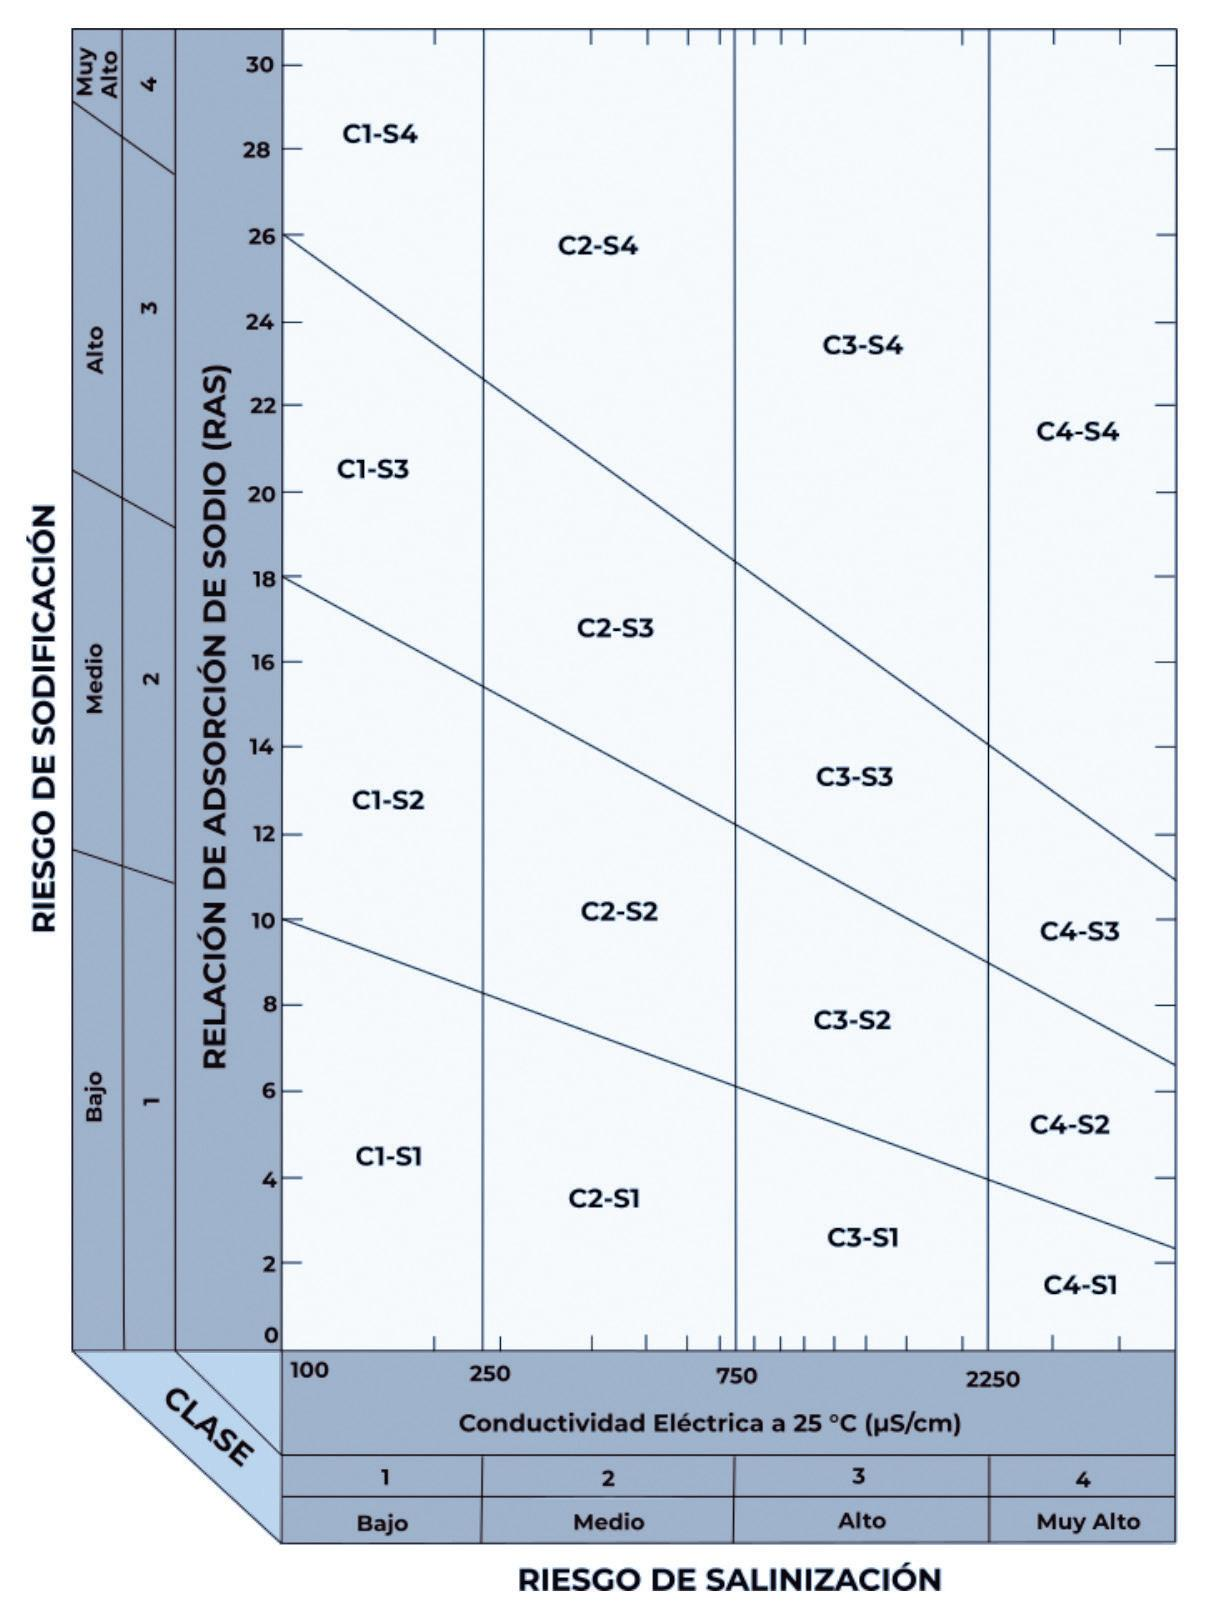
\includegraphics[width=0.5\textwidth]{sa1.jpg}
  \caption{Clasificación de salinidad y sodicidad para las aguas de riego USLD-USDA}
  \label{sa1}
\end{figure}
En el diagrama del Manual 60 se indica que el peligro potencial de sodificación manifestado a través del valor del RAS, es más alto a medida que aumenta la concentración de solutos, por ejemplo, si la CE vale 380 micromhos/cm y el RAS 14 el agua tendría una clasificación de C2S2. En cambio, para el mismo RAS de 14 y un valor de CE de 3,000 micromhos/cm, el agua tendría una clasificación de C4S4.

Esta propuesta no la comparten el autor y otros investigadores, ya que consideran que al incrementarse el contenido de solutos en la solución del suelo también se aumenta el número de cargas libres positivas de los cationes en solución, que aunque no formen parte del complejo de intercambio, pueden reducir la cantidad de cargas negativas que quedan libres y, por tanto, producir un efecto floculante en el suelo, atenuando las consecuencias dispersantes del sodio sobre su estructura, la inclinación de las rectas de los valores de RAS en el diagrama del Manual 60

La inclinación de las rectas debería estar invertida, deberían estar hacia arriba, por lo que no se recomienda el nomograma del Manual 60

Estos investigadores propusieron una guía para la interpretación de análisis de agua para riego, en donde combinan el RAS con la CE para definir varias clases de agua
\begin{table}[h!]
  \centering
  \begin{tabular}{@{}cccc@{}}
  \toprule
  \multirow{3}{*}{RAS} & \multicolumn{3}{c}{Grado de restricción de uso}                                                \\ \cmidrule(l){2-4} 
                       & Severo        & \begin{tabular}[c]{@{}c@{}}Ligero a\\ moderado\end{tabular} & Ningúno          \\
                       & \multicolumn{3}{c}{CE (dS/m)}                                                                  \\ \midrule
  0 - 3                & \textless 0.2 & 0.2 - 0.7                                                   & \textgreater 0.7 \\
  3 - 6                & \textless 0.3 & 0.3 - 1.2                                                   & \textgreater 1.2 \\
  6 - 12               & \textless 0.5 & 0.5 - 1.2                                                   & \textgreater 1.9 \\
  12 - 20              & \textless 1.3 & 1.3 - 2.9                                                   & \textgreater 2.9 \\
  20 - 40              & \textless 2.9 & 2.9 - 5.0                                                   & \textgreater 5.0 \\ \bottomrule
  \end{tabular}
  \caption{Norma combinada de Ayers y Westcot, de 1989}
  \label{tabs8}
\end{table}
\begin{figure}[h!]
\centering
  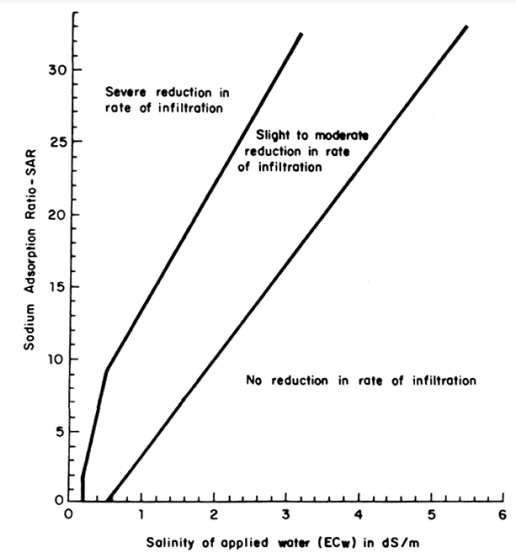
\includegraphics[width=0.5\textwidth]{sa2.png}
  \caption{Reducción relativa de la infiltración provocada por la salinidad y la relación de adsorción de sodio}
  \label{sa2png}
\end{figure}
\subsubsection{Carbonato de sodio residual (CSR)}
Este índice fue desarrollado con la finalidad de predecir la tendencia a precipitarse
que pueden tener las sales de carbonato de calcio y magnesio en el suelo, lo que
debido a su muy baja solubilidad, puede suceder cuando se reduce el contenido de
humedad, condición que propiciaría que queden las de sodio en la solución del suelo
por ser más solubles. Esto puede incrementar el riesgo de sodificación, ya que se
disminuye la participación del calcio en el complejo de intercambio y se aumenta la
proporción relativa de sodio presente en el suelo y, por tanto, el valor de RAS, a
pesar de no variar la cantidad de sodio presente

La fórmula para calcular el CSR es la siguiente (Eaton, 1950):
\begin{equation}
  CSR = (CO_3 + HCO_3) - (Ca + Mg)
\end{equation}
Las tres clases que se utilizan para este índice son:
\begin{table}[h!]
  \centering
  \begin{tabular}{@{}ccc@{}}
  \toprule
  Clase & Calidad de acuerdo al CSR                      &  \\ \midrule
  1     & \textless 1.25 (Uso sin peligro)               &  \\
  2     & 1.25 - 2.5 (Condicionadas)                     &  \\
  3     & \textgreater 2.5 (No recomendables para riego) &  \\ \bottomrule
  \end{tabular}
  \caption{Carbonato de sodio residual (CSR)}
  \label{tabs9}
\end{table}
\subsubsection{Relación de adsorción de sodio ajustado (adj Rna}
Es una modificación del RAS, que permite predecir mejor los peligros asociados con el sodio y los problemas potenciales sobre la capacidad de infiltración del suelo por la presencia de sodio en el agua de riego, tomando en cuenta los mismos fundamentos utilizados por Eaton, respecto a que la evapotranspiración puede propiciar una precipitación de carbonatos y bicarbonatos de calcio. Es decir, considera que la concentración de calcio en la interfase suelo-agua no es constante y depende tanto de dicha concentración en el agua de riego como de la disolución o la precipitación del calcio en el suelo.

La adj RNa puede calcularse mediante la siguiente expresión Ayers y Westcot (1987) en meq/l:
\begin{equation}
  adj\,Rna = \frac{Na}{\sqrt{\frac{Ca + Mg}{2}}}
\end{equation}
\subsubsection{Porcentaje de Sodio Soluble (PSS)}
El PSS es el índice más sencillo y directo que existe para evaluar el peligro potencial
del sodio. Se define como el porcentaje que tiene el sodio en relación con la cantidad
total de cationes solubles y su fórmula es la siguiente (Wilcox 1955):
\begin{equation}
PSS = \frac{(Na \times 100)}{(Na + Ca + Mg + K)} 
\end{equation}
\begin{table}[h!]
  \centering
  \begin{tabular}{@{}cc@{}}
  \toprule
  \begin{tabular}[c]{@{}c@{}}PSS\\ (\%)\end{tabular} & Calidad    \\ \midrule
  \textless 20                                       & Excelente  \\
  20 - 40                                            & Buena      \\
  40 - 60                                            & Permisible \\
  60 - 80                                            & Dudosa     \\
  \textgreater 80                                    & Inapta     \\ \bottomrule
  \end{tabular}
  \caption{Porcentaje de Sodio Soluble (PSS)}
  \label{tabsa10}
  \end{table}
\subsubsection{Relación de calcio o Índice de Kelly}
Evalúa el riesgo de alcalinización del suelo en función de la relación que existe entre
el calcio y el total de cationes. Se expresa en porcentaje y se calcula mediante la
siguiente fórmula (Kelly 1955):
\begin{equation}
  I.K. = \frac{Ca}{(Ca + Mg + Na) \times 100}
\end{equation}
\begin{table}[h!]
  \centering
  \begin{tabular}{@{}cc@{}}
  \toprule
  \begin{tabular}[c]{@{}c@{}}Índice de\\ Kelly\end{tabular} & \begin{tabular}[c]{@{}c@{}}Calidad del\\ agua\end{tabular} \\ \midrule
  \textless 35 \%    & Mala   \\
  35 \%              & Dudosa \\
  \textgreater 35 \% & Buena  \\ \bottomrule
  \end{tabular}
  \caption{Relación de calcio o Índice de Kelly}
  \label{tabsa11}
  \end{table}
\subsubsection{Porciento de sodio posible (PSP)}
Indica el peligro de desplazamiento o sustitución del Ca y del Mg por el Na en el complejo de intercambio, que se inicia cuando el contenido de Na en solución representa más del 50\% de los cationes disueltos, resaltando que es poco usado y se calcula mediante la siguiente fórmula (citado por Aceves 2011) Na en meq/lt:
\begin{equation}
  PSP = (Na / SE) \times  100
\end{equation}
Scofield estableció que valores de PSP mayores a 60\% eran peligrosos, y posteriormente Green en 1984 subió este índice hasta 80\%

\subsubsection{Índice de permeabilidad (IP)}
Es una estimación empírica de la probable afectación de la permeabilidad del suelo por el efecto del sodio y también es poco usado, y se clasifica de acuerdo con el diagrama de Doneen, y se calcula mediante la siguiente fórmula (Doneen, 1964)
\begin{equation}
  IP = \frac{\left(Na + \sqrt{HCO_3}\right) \times 100}{\left(Ca + Mg + Na\right)}
\end{equation}
Los valores para las diferentes clases de este índice son:
\begin{table}[h!]
  \centering
  \begin{tabular}{@{}ccc@{}}
  \toprule
  Clase & Calidad de acuerdo al CSR                        &  \\ \midrule
  1     & \textless 50\% (Uso sin peligro)                 &  \\
  2     & 50 - 100\$ (Condicionadas)                       &  \\
  3     & \textgreater 100\% (No recomendables para riego) &  \\ \bottomrule
  \end{tabular}
  \caption{Índice de permeabilidad (IP)}
  \label{tabsa12}
  \end{table}
Aunque no es un índice directo para evaluar el peligro potencial del sodio en el agua de riego, es una muy buena referencia que permite verificar dicho peligro de manera indirecta, ya que la presencia de carbonatos y bicarbonatos de sodio incrementan de manera significativa el pH del suelo, de tal manera que un alto valor de pH del agua, especialmente superiores a 7.5, indica un mayor peligro potencial de sodificación.
\subsection{Índices para definir la fitoxicidad o efectos tóxicos de algunos iones específicos}
Los principales índices o iones específicos para determinar la fitotoxicidad de un
agua de riego son Salinidad Potencial, cloruros, sodio, boro y bicarbonatos .
\subsubsection{Salinidad potencial (SP)}
Estima el peligro potencial tóxico de los cloruros y sulfatos, por ser los solutos más solubles y ser las últimas sales que quedan en solución una vez precipitadas las menos solubles, que son los carbonatos y bicarbonatos. Se estima con la siguiente fórmula Doneen, (1964), en meq/l:
\begin{equation}
  SP = Cl + \frac{a}{2}SO_4 
\end{equation}
\subsubsection{Cloruros}
Es la fitotoxicidad específica más común que existe de todos los iones, debido a su predominancia en la mayoría de las aguas de riego, por lo que cuando la concentración de cloruros en ellas excede la tolerancia de la planta se presentan síntomas de toxicidad. Las clases son las siguientes.
\begin{table}[h!]
  \centering
  \begin{tabular}{@{}cc@{}}
  \toprule
  Clase           & \begin{tabular}[c]{@{}c@{}}Contenido\\ de cloruros\\ (me/l)\end{tabular} \\ \midrule
  Buena           & menos de 4                                                               \\
  Condicionada    & de 4 a 10                                                                \\
  No recomendable & más de 10                                                                \\ \bottomrule
  \end{tabular}
  \caption{Cloruros}
  \label{tabsa13}
\end{table}
\subsubsection{Sodio}
La respuesta de las plantas al sodio varía, dependiendo de la especie y de las condiciones de salinidad y sodicidad, ya que su concentración en la solución del suelo puede alcanzar niveles desproporcionalmente altos en relación con el K y la raíz debe enfrentarse a las altas concentraciones de sodio y altos potenciales osmóticos, por lo que la capacidad de la planta para ajustarse y adaptarse a condiciones de exceso de sodio, determina su capacidad de crecimiento y desarrollo.

Las clases basadas en el valor del RAS son:
\begin{table}[h!]
  \centering
  \begin{tabular}{@{}cc@{}}
  \toprule
  Clase                & \begin{tabular}[c]{@{}c@{}}RAS\\ (meq/l)\end{tabular} \\ \midrule
  Sin problema         & menos de 3                                            \\
  Problemas crecientes & de 3 a 9                                              \\
  Problemas severos    & más de 9                                              \\ \bottomrule
  \end{tabular}
  \caption{Sodio}
  \label{tabsa14}
\end{table}
\subsubsection{Boro}
Algunas aguas de riego pueden contener exceso de boro desde su origen o por
contaminación con aguas residuales urbanas e industriales, pudiendo afectar a los
cultivos.

Las clases son:
\begin{table}[h!]
  \centering
  \begin{tabular}{@{}cc@{}}
  \toprule
  Clase                & Boro(meq/l)  \\ \midrule
  Sin problema         & menos de 0.7 \\
  Problemas crecientes & de 0.7 a 3   \\
  Problemas severos    & más de 3     \\ \bottomrule
  \end{tabular}
  \caption{Boro}
  \label{tabsa15}
\end{table}

\subsubsection{Bicarbonatos}
Aunque los bicarbonatos generalmente no se presentan en altas cantidades en las
aguas de riego, existen algunos reportes de que cuando sucede y se combina con
altas presencias de sodio, afectan a la mayoría de los cultivos.

Las clases son:
\begin{table}[h!]
  \centering
  \begin{tabular}{@{}cc@{}}
  \toprule
  Clase                & \begin{tabular}[c]{@{}c@{}}$HCO_3$\\ (meq/l)\end{tabular} \\ \midrule
  Sin problema         & menos de 1.5                                              \\
  Problemas crecientes & de 1.5 a 8.5                                              \\
  Problemas severos    & más de 8.5                                                \\ \bottomrule
  \end{tabular}
  \caption{Bicarbonatos}
  \label{tabsa16}
\end{table}
\subsubsection{Efectos nutricionales misceláneos}
La interacción de la salinidad con la absorción y utilización de nutrientes tiene muchas implicaciones prácticas, relacionadas principalmente con el tipo y concentración de solutos presentes en el agua, con los fertilizantes a usar, con el tipo de cultivo y su capacidad de adaptación a condiciones salinas, y con la influencia de la salinidad en la nutrición de iones como N, Ca, K y P.

Por tanto, los excesos de sales o la presencia de determinados iones en el agua de riego, pueden inducir desbalances o deficiencias nutricionales en los cultivos y afectar los rendimientos.

\subsubsection{Criterio agronómico de la calidad del agua de riego}
Es un concepto que se aplica única y exclusivamente cuando el agua de riego
presenta algún tipo de problema en su calidad química.
Se refiere a la búsqueda por un especialista en riego, de alternativas y propuestas
para poder utilizar y aprovechar dicha agua “problemática” para fines productivos
agropecuarios, lo que se puede lograr mediante un manejo planificado, integrado y
particularizado de esa agua de riego, tomando en cuenta los diferentes factores o
componentes agronómicos que intervienen, por ejemplo:
\begin{enumerate}
  \item La selección de cultivos tolerantes y el control de la salinidad del suelo mediante el drenaje.
  \item El mantenimiento de las propiedades físicas del suelo para asegurar una adecuada infiltración y permeabilidad, según sean los requerimientos hídricos del cultivo y garantizando la aireación de las raíces.
  \item La adopción de técnicas adecuadas de riego, y,
  \item La disponibilidad de métodos adecuados de drenaje.
\end{enumerate}
Los principales factores que el autor considera para aplicar el Criterio Agronómico, son el requerimiento de lavado o sobre-riego, la textura del suelo, el cultivo, el método de riego, el manejo integrado del proceso productivo, el drenaje de los suelos y el mejoramiento de la calidad química del agua.
\section{Acumulación de sales de los suelos}
Procesos de acumulación de sales de los suelos y principles problemas de salinización que se presentan en las áreas bajo riego en México
\subsection{Orígen y fuente de las sales solubles presentes en aguas y suelos}
\subsubsection{Sales presentes en aguas y suelos}
Las ``sales'' presentes en un suelo agrícola bajo riego pueden encontrarse en general en dos formas, ya sea disueltas en la solución o retenidas en el complejo de intercambio, condición que cambia continuamente al irse modificando el régimen de humedad del suelo, pudiendo pasar las sales de una posición a otra. En algunos pocos casos de suelos muy fuertemente afectados por sales, se pueden encontrar en forma precipitada como cristales.

En la práctica y de manera convencional, se utiliza el término “sal” para identificar a los componentes químicos que existen en solución en las aguas de riego y, posteriormente, en los suelos agrícolas después de regarlos, lo que en realidad no corresponde a la definición química de sal que se refiere al compuesto o producto que resulta de la reacción entre un ácido y una base.

Es decir, los elementos químicos presentes en las aguas y suelos dejaron de ser sales debido a que ya no forman un compuesto, puesto que pasaron a ser solutos o iones en solución, encontrándose estos en forma disociada o disuelta ya sean como aniones (carga negativa) o como cationes (carga positiva).

\subsubsection{Origen y fuente de ls aniones y cationes solubles presentes en aguas y suelos}
El origen o fuente de todos los aniones y cationes solubles presentes en las aguas y posteriormente en los suelos bajo riego, son las rocas y minerales que forman parte de la corteza terrestre, los cuáles son liberados de ellos como consecuencia de los procesos naturales de intemperismo o meteorización propiciados por agentes naturales como el ciclo hidrológico y el clima.

Los principales tipos de intemperismo son los químicos y los físicos.
\begin{itemize}
  \item Químicos. Son los de solución o solubilización, oxidación, hidrólisis, hidratación, deshidratación, carbonatación y reducción.
  \item Físicos. Son el humedecimiento y secado, el calentamiento y enfriamiento, el congelamiento del agua, la lluvia y la erosión hídrica, la erosión eólica, la acción de los glaciares, la acción de las olas, principalmente.  
\end{itemize}
El agua es el factor que más participa en la mayoría de estos procesos, siendo el químico de solubilización el más importante de todos ellos.

La gran dinámica natural que tiene el movimiento del agua dentro del ciclo hidrológico, especialmente la que se precipita como lluvia sobre los continentes y la que se deshiela de sus partes altas, propicia que parte de dicha agua pueda o evapotranspirarse, o escurrir sobre la superficie para almacenarse en algún cuerpo de agua o desfogarse al mar, o penetrar en el suelo para retenerse en él o infiltrarse hacia estratos inferiores.

La tasa o magnitud de cada uno de estos procesos dependerá principalmente del clima e intensidad de la precipitación o deshielo, cobertura vegetal, permeabilidad del material geológico superficial o suelo, de la pendiente y de la época del año.

En los casos de las aguas que escurren y las que se infiltran en forma líquida por efecto de la gravedad, sufren cambios en su composición química a través de todo su recorrido al entrar en contacto con las rocas y minerales, que consisten en un enriquecimiento de solutos debido al alto poder de solubilización del agua, que son transportados del sitio donde son extraídos de los minerales hasta donde se riega.

\subsubsection{Factores que definen el tipo de solutos}
Los factores que participan son dos, el primero es el grado de facilidad que tienen
los elementos para liberase de los minerales y el segundo es que tanta abundancia
existe de ellos en los principales constituyentes químicos de la corteza terrestre, los
cuáles se presentan y explican adelante.
Otros factores que también participan, pero en un mínimo grado y que sólo se
mencionarán, son los inducidos por el hombre como los siguientes.
\begin{itemize}
  \item Las descargas de aguas residuales o de drenaje de áreas bajo riego en corrientes superficiales
  \item Las filtraciones en el suelo de aguas residuales o de drenaje de áreas bajo riego
  \item La sobreexplotación de los acuíferos, que puede ocasionar su contaminación por mantos salinos contiguos o por intrusión salina en aquellos ubicados cerca de las costas.
\end{itemize}

\textbf{ Grado de facilidad que tienen los elementos para liberarse de los minerales:}

Esta facilidad depende principalmente de la solubilidad que tiene un elemento y del tipo de compuesto del cual forman parte.

En este contexto, Kovda, en 1974 definió unas categorías del grado o facilidad que tienen algunos elementos o cationes de desprenderse o liberarse de los minerales (no incluye a los aniones)
\begin{table}[h!]
  \centering
  \begin{tabular}{@{}cc@{}}
  \toprule
  Categorías               & Elementos                 \\ \midrule
  Muy altamente lavables   & Cl, Br, I, S, C, B        \\
  Altamente lavables       & Na, K, Ca, Mg, Cu, Co, Zn \\
  Lavables                 & P, Mn                     \\
  Ligeramente lavables     & Fe, Al, Si                \\
  Virtualmente no lavables & Si (del cuarzo)           \\ \bottomrule
  \end{tabular}
  \caption{Grado de facilidad que tienen los elementos para liberarse de los minerales}
  \label{tabsa17}
 \end{table}
\textbf{Abundancia de los principales constituyentes químicos de la corteza terrestre}
El segundo factor que define los diferentes elementos que se encuentran presentes en las aguas de riego, es el porcentaje total de ellos que están como componentes en los aproximadamente 2,000 minerales primarios que se estima existen en la corteza terrestre y los porcentajes de los principales componentes químicos de los minerales presentes en ella, son
\begin{table}[h!]
  \centering
  \begin{tabular}{@{}cccc@{}}
  \toprule
  ELEMENTO & \%    & ELEMENTO  & \%   \\ \midrule
  Oxígeno  & 46.50 & Magnesio  & 2.10 \\
  Silicio  & 27.60 & Titanio   & 0.60 \\
  Aluminio & 8.10  & Fósforo   & 0.12 \\
  Fierro   & 5.10  & Manganeso & 0.09 \\
  Calcio   & 3.60  & Azufre    & 0.06 \\
  Sodio    & 2.80  & Cloro     & 0.05 \\
  Potasio  & 2.60  & Carbono   & 0.04 \\ \bottomrule
  \end{tabular}
  \caption{Abundancia de los principales constituyentes químicos de la corteza terrestre}
  \label{tabsa18}
  \end{table}
\textbf{Principales iones presentes en las aguas de riego}
Se detecta que los elementos que existen en mayor abundancia son el oxígeno y el silicio, ya que constituyen el 74\% del total y le siguen el aluminio, el fierro, el calcio, el sodio, el potasio y el magnesio, que constituyen un 24%y en su conjunto estos ocho elementos representan más de 98\% del total de la composición química de la corteza terrestre.

Al combinar los datos de abundancia con el grado de facilidad que tienen los elementos para liberarse de los minerales, se explica el por qué los aniones cloruros, los sulfatos, los carbonatos y bicarbonatos y los cationes sodio, calcio, magnesio y potasio, son los que están presentes en la mayoría de las aguas que se utilizan para riego y, como consecuencia, los que predominan en los suelos bajo riego, como se complementa a continuación.

\textbf{Principales iones presentes en las aguas superficiales y en los acuíferos}
\begin{enumerate}
  \item \textbf{Aguas de riego cuya fuente de abastecimiento son las corrientes
  superficiales.} Los principales aniones y cationes que de manera general
  predominan en estas aguas, son en orden decreciente: \begin{enumerate}
    \item Aniones. En orden de importancia son los cloruros, los sulfatos, carbonatos y bicarbonatos. También se puede presentar el boro y algunos otros en mínimas cantidades.
    \item Cationes. En orden de importancia son el sodio, calcio, magnesio y el potasio. También se pueden presentar los nitratos y algunos otros en cantidades despreciables.
  \end{enumerate}
  \item \textbf{Aguas de riego que provienen de los mantos acuíferos}. Las aguas subterráneas, por tener contacto con una mayor diversidad de minerales que las superficiales, presentan más variabilidad en sus componentes químicos que las superficiales, por lo que la predominancia de un anión o catión depende de la zona o región por donde circularon.
\end{enumerate}
El principal factor es el tiempo de contacto que tiene el agua con los minerales por donde circula y, en segundo lugar, el tipo de minerales con el que tiene contacto.

\subsubsection{Tiempo de contacto con los minerales}

En general, entre mayor tiempo de contacto con los minerales del agua que circula, es mayor la cantidad de sales que pueden disolverse, tiempo que a su vez depende de dos subfactores, la velocidad con la que circula y la distancia que recorre.
\begin{itemize}
  \item \textbf{Velocidad del agua}. 
  
  Cuanto mayor sea la velocidad con la que circula el agua, menor será el tiempo de contacto con los minerales y, por tanto, habrá menor solubilización de sales y menor concentración de solutos en el agua. Dicha velocidad la determina el tipo de recorrido que realiza el agua, que puede ser superficial o subterráneo, por lo que, tomando en cuenta que las aguas que escurren superficialmente lo hacen a una velocidad muchas veces mayor que las que se infiltran y circulan subterráneamente, las aguas superficiales siempre presentarán concentraciones de solutos mucho menores que las subterráneas.
  \item \textbf{Distancia de recorrido del agua}. 
  
  Este factor es menos determinante que el de la velocidad de recorrido y se aplica principalmente a las aguas superficiales, debido a que recorren grandes distancias, a diferencia de las subterráneas que recorren distancias más cortas. Así, en el caso de las corrientes superficiales, a mayor distancia de recorrido más tiempo de contacto con los minerales y, por tanto, más solubilización de sales y mayor concentración de solutos en el agua. Un factor que también participa relacionado con la distancia de recorrido de las aguas superficiales, es la evaporación, la cual incrementa la concentración de solutos al aumentar la distancia, aunque mínimamente.
\end{itemize}
\subsubsection{Tipo de minerales con los que el agua tiene contacto durante su recorrido}
La composición química de los minerales con los que el agua tiene contacto a través de su recorrido y el grado de solubilización de estos, determina la facilidad con la cual sus componentes pueden liberarse de ellos y pasar a formar parte del agua que circula, lo que a su vez influye en la concentración de solutos de dicha agua.
\begin{table}[h!]
  \centering
  \begin{tabular}{@{}ccc@{}}
  \toprule
  \begin{tabular}[c]{@{}c@{}}Macro\\ Elemento\end{tabular} &
    Función &
    \begin{tabular}[c]{@{}c@{}}Se absorbe\\ en forma de:\end{tabular} \\ \midrule
  C,H, y O &
    \begin{tabular}[c]{@{}c@{}}Son nutrientes no minerales y forman parte de todas las moléculas biológicas\\ u orgánicas\end{tabular} &
    $CO2$ \\
  N &
    \begin{tabular}[c]{@{}c@{}}Es aprovechado sólo como nitrito, nitrato y amonio y es constituyente básico\\ de las proteínas, la clorofila, las enzimas, aminoácidos y nucleótidos\end{tabular} &
    \begin{tabular}[c]{@{}c@{}}$(NO_3)^{-1}$\\ $(NH_4)^{+1}$\end{tabular} \\
  P &
    \begin{tabular}[c]{@{}c@{}}Es necesario en todos los procesos de intercambio de energía, formando\\ parte del ATP y de los nucleótidos y lípidos que forman las membranas; su\\ déficit detiene el crecimiento, atrofia las raíces y detiene la madurez\end{tabular} &
    \begin{tabular}[c]{@{}c@{}}$(HPO_4)^{-2}$\\ $(H_2PO_4)^{-1}$\end{tabular} \\
  K &
    \begin{tabular}[c]{@{}c@{}}Interviene en el equilibrio osmótico e iónico y en la activación de un gran\\ número de enzimas\end{tabular} &
    $K^{+1}$ \\
  Ca &
    \begin{tabular}[c]{@{}c@{}}Forma parte de la pared celular, regula la permeabilidad celular y es\\ indispensable para el crecimiento de las raíces y combinado con quitina\\ presta rigidez a las células\end{tabular} &
    $Ca^{+2}$ \\
  Mg &
    \begin{tabular}[c]{@{}c@{}}Forma parte integral de la molécula de clorofila, indispensable para la\\ fotosíntesis\end{tabular} &
    $Mg^{+2}$ \\
  S &
    Es constituyente básico de las proteínas y algunos aminoácidos &
    $(SO_4)^{-2}$ \\
  Mn &
    \begin{tabular}[c]{@{}c@{}}Activa enzimas importantes para el catabolismo y es necesario para la liberación de\\ oxígeno durante la fotosíntesis; facilita la transferencia de electrones en ella\end{tabular} &
    $Mn^{+2}$ \\
  Cu &
    Activa ciertas enzimas e influye en el metabolismo &
    $Cu^{+2}$ \\
  Fe &
    \begin{tabular}[c]{@{}c@{}}Interviene en la producción de clorofila y en muchas moléculas que transportan\\ oxígeno y electrones\end{tabular} &
    \begin{tabular}[c]{@{}c@{}}$Fe^{+3}$\\ $Fe^{+2}$\end{tabular} \\
  Zn &
    \begin{tabular}[c]{@{}c@{}}Activador o componente de muchas enzimas e interviene en la síntesis de\\ hormonas vegetales que regulan el crecimiento\end{tabular} &
    $Zn^{+2}$ \\
  Na &
    Es necesario para el equilibrio ácido-base e interviene en los procesos osmóticos &
    $Na^{+1}$ \\
  B &
    \begin{tabular}[c]{@{}c@{}}Interviene en la división celular, el metabolismo de los carbohidratos, el metabolismo\\ del agua, el transporte de azúcares y la germinación; su déficit inhibe el crecimiento\\ y ocasiona que las hojas se tornen amarillas\end{tabular} &
    \begin{tabular}[c]{@{}c@{}}$(H_2BO_3)^{-1}$\\ $(HBO_3)^{-2}$\\ $(BO_3)^{-3}$\end{tabular} \\
  Co &
    \begin{tabular}[c]{@{}c@{}}Forma parte de algunos transportadores de electrones y de algunas enzimas;\\ además, Interviene en la síntesis de vitamina B\end{tabular} &
    $Co^{+2}$ \\
  Mo &
    Es un catalizador que favorece la fijación bacteriana de nitrógeno &
    $(MoO_4)^{-2}$ \\
  Cl &
    \begin{tabular}[c]{@{}c@{}}Protege los fotosistemas de componentes oxidantes y facilita la transferencia de\\ electrones del agua a la clorofila\end{tabular} &
    $Cl^{-1}$ \\
  Ni &
    Forma parte de la enzima ureasa que disocia la urea en $CO_2$ y $NH_4^{+1}$ &
    $Ni^{+2}$ \\ \bottomrule
  \end{tabular}
  \caption{Principales nutrientes esenciales}
  \label{tabsa19}
\end{table}

\subsection{Procesos de acumulación de sales de los suelos}
Son aquellos que se originan por causas naturales en todo el mundo, y que implican tanto ciclos de liberación in situ de sales de rocas y minerales, como de movilización, redistribución y acumulación por diferentes medios y a cierta distancia de su lugar de origen, lo cual depende de las características del sitio o cuenca en donde se presentan.

Los principales son los siguientes:
\begin{itemize}
  \item Ciclos marinos de acumulación de sales
  \item Mares internos
  \item Cuencas cerradas o endorreica
  \item Ciclos deltaicos
  \item Ciclos artesianos
\end{itemize}
\subsection{Procesos de ensalitramiento inducidos en las áreas bajo riego}
Se deben principalmente al desconocimiento técnico de las causas que los propician, así como por la falta de una planeación adecuada en el manejo y uso del agua de riego.

Un factor natural que está correlacionado e influye en los procesos de ensalitramiento en un suelo, es que las áreas que se incorporan a una agricultura bajo riego se localizan en su mayoría en zonas áridas o semiáridas, en donde la evapotranspiración es varias veces mayor que la precipitación, situación que favorece la acumulación de sales.

Dicha incorporación de áreas al riego está plenamente justificada, debido a que su finalidad es la de satisfacer necesidades primordiales del ser humano, pero no existen argumentos válidos para explicar el por qué, a pesar de que se conoce con antelación que la aplicación de riegos invariable e inevitablemente conduce al ensalitramiento del suelo o de algún otro lugar, esto sigue ocurriendo.

\subsection{Proceso de ensalitramiento directo, primario o por arriba}
Es el menos frecuente a nivel mundial y se presenta debido a que todas las aguas de riego contienen sales en solución, y en teoría el 99\% del agua aplicada se evapotranspira, quedándose en el suelo la mayoría de los solutos que contiene el agua de riego.

Por ejemplo, si en un ciclo agrícola se aplica a un cultivo una lámina total de riego de 90 cm y la concentración de sales del agua es de 500 ppm o mg/l, al final de ese ciclo se quedarían en una hectárea un poco menos de 4.5 toneladas de sales, por lo que al regar sucesivamente dicha parcela se propicia su acumulación en el suelo a través del tiempo.

Por tanto, en los suelos bajo riego en general siempre existirá un contenido de sales de 2 a 4 veces mayor que los que tiene el agua de riego que se utilice, lo que depende principalmente de su manejo, ya que para que el suelo tuviera un contenido semejante al del agua de riego tendrían que existir condiciones hipotéticas de cero evapotranspiración combinado con un flujo continuo de agua.

El conocimiento de este proceso directo de ensalitramiento motivó el desarrollo de
un procedimiento o vacuna para prevenirlo, que se conoce como Requerimiento de
Lavado (RL), por lo que un proceso directo se
presenta simple y llanamente cuando no se aplica dicho RL, que puede deberse a
las siguientes causas.
\begin{itemize}
  \item La principal es por el desconocimiento del usuario de que tiene que aplicarlo cuando un agua de riego presenta ciertas concentraciones elevadas de sales, especialmente cuando se utilizan aguas de riego con calidades de tercera y cuarta clase de CE, que implican elevados valores de RL
  \item Por limitaciones existentes en la disponibilidad de agua o porque el agua de riego tiene un alto costo, motivando que el usuario se resista a aplicarla
  \item Cuando se combina altas concentraciones de sales en el agua con una alta eficiencia en los métodos de riego que se utilizan, especialmente en los localizados.
\end{itemize}
Como ejemplos de México en donde ha sucedido este caso y que se detallan más
adelante, son:
\begin{itemize}
  \item Los cuatro Distritos de Riego de México que están ubicados colindantes al mar en donde utilizan agua subterránea que se contaminó por intrusión salina, propiciando con ello un incremento paulatino de la concentración de sales en el agua de riego, lo que, combinado con la no aplicación del RL requerido, ha salinizado de manera directa los suelos.
  \item El Distrito de Riego de Mexicali, cuyas aguas de riego, tanto de gravedad como de bombeo, presentan elevados contenidos de sales.
  \item Algunos Distritos y Unidades de Riego ubicados en Valles Centrales no colindantes a la costa, en donde también se ha presentado la contaminación de aguas por la sobreexplotación de acuíferos, posibilidad que también puede suceder a futuro en las Unidades de Riego por bombeo de la Península de Yucatán.
\end{itemize}
\subsection{Proceso de ensalitramiento indirecto, secundario o por abajo}
Es el que más frecuentemente se presenta en las áreas de riego, teniendo como causa general la combinación de un uso y manejo ineficiente del agua de riego que propicia pérdidas de agua por infiltración profunda hacia estratos inferiores, con condiciones no adecuadas de drenaje de los suelos, ya sean naturales o artificiales.

Se estima que las pérdidas en las áreas que se riegan con métodos por gravedad fluctúan entre el 40 y 60\%, lo que provoca la elevación de los niveles freáticos, lo que favorece que el agua freática con sales en solución asciendan por capilaridad a la superficie, en donde solamente se evapora el agua y, por tanto, permanezcan la mayoría de las sales, las cuáles pueden acumularse hasta ensalitrar el suelo

Un factor de raíz que contribuye a que se presente este tipo de proceso, es que al incorporar al riego áreas ubicadas en zonas áridas y semiáridas, se altera el régimen hídrico original de los suelos, al entrar una mayor cantidad de agua de la que recibían antes, ocasionando con ello que se rebase la capacidad natural de drenaje de los suelos y, por ello, si no se construye suficiente drenaje artificial general o parcelario, se propicia la elevación de los niveles freáticos.

\textbf{Causas directas}:
\begin{enumerate}
  \item Causas directas que propician las pérdidas de agua por infiltración profunda \begin{enumerate}
    \item Insuficiente o inadecuada infraestructura hidráulica.
    \item Una operación no adecuada de la infraestructura hidráulica y una
    \item La utilización mayoritaria de métodos de riego por gravedad. insuficiente o inadecuada conservación de dicha infraestructura hidráulica.
    \item La no medición precisa de entrega del agua de riego a los usuarios en la entrada de cada parcela por la falta de equipos de control y lectura.
    \item Insuficiente tecnificación del riego o falta de ella.
    \item Limitaciones financieras para infraestructura, para su adecuada operación y conservación, para su modernización, y para la tecnificación del riego por gravedad
    \item La superficie total de riego del Distrito.
    \item El volumen total de agua anual utilizado para riego en un área de riego.
  \end{enumerate}
  \item Causas directas que coadyuvan a la elevación de los niveles freáticos y a ocasionar problemas de drenaje interno en los suelos \begin{enumerate}
    \item Insuficiente o inadecuada infraestructura de drenaje artificial, tanto de la red general como parcelario y una insuficiente .o inadecuada conservación de la misma.
    \item Limitaciones financieras, tanto para construir el drenaje requerido, como para llevar a cabo una adecuada operación, conservación y modernización de él.
    \item Parcelas de riego ubicadas colindantes a cuerpos lacustres o a las costas
  \end{enumerate}
\end{enumerate}

Causas indirectas o coyunturales que coadyuvan a la elevación de los niveles freáticos y a ocasionar problemas de drenaje interno en los suelos
\begin{enumerate}
  \item Deficiente cultura del agua y de la legalidad.
  \item Bajos precios del agua de riego.
  \item La no aplicación de la legislación vigente.
  \item Falta de una legislación más estricta y motivante
  \item Esquemas inadecuados y poco estrictos de dotación y entrega del agua de riego al productor.
\end{enumerate}
\begin{table}[h!]
  \centering
  \begin{tabular}{@{}cc@{}}
  \toprule
  \multicolumn{2}{c}{Causa y efecto}                                                \\ \midrule
  General              & Uso y manejo ineficiente del agua de riego                 \\
  Primaria / primario  & Pérdidas de agua por filtración profunda                   \\
  Secundaria /  primario & \begin{tabular}[c]{@{}c@{}}Elevación de los niveles freáticos y problemas de drenaje\\ \\ interno de los suelos\end{tabular} \\
  Terciaria / primario & Presencia de niveles freáticos someros                     \\
  Cuaternaria / primario & \begin{tabular}[c]{@{}c@{}}Ascenso de agua freática por capilaridad a la superficie\\ del suelo\end{tabular}                 \\
  Quinaria / primario  & Evaporación del agua freática que asciende a la superficie \\
  Final                & Acumulación de sales y el ensalitramiento de los suelos    \\ \bottomrule
  \end{tabular}
  \caption{Causas y efectos en el ensalitramiento indirecto, secundario o por abajo}
  \label{tabsa20}
\end{table}
\section{Caracterización y clasificación de suelos con problemas de sales y mantos freáticos someros}
La caracterización es la metodología que hay que seguir para distinguir y precisar las características y atributos particulares relacionados con el problema de salinidad que presentan las áreas estudiadas en un momento dado.

Su finalidad es detallar el tipo e intensidad de la problemática de salinidad que existe, lo que incluye la diferenciación, delimitación y cuantificación de las áreas ensalitradas, así como la determinación de las propiedades del suelo involucradas y la identificación de las causas que originaron o están originando el problema.

La información que se obtenga con la caracterización permitirá lo
siguiente:
\begin{enumerate}
    \item Conocer a detalle el problema de salinidad agrícola de una parcela o de una cierta área de estudio, así como las causas que lo originaron y su situación actual.
    \item Clasificar el problema de ensalitramiento.
    \item Emitir un diagnóstico del problema de salinidad del suelo que incluya el grado de dificultad que puede tener la recuperación del mismo.
    \item Elaborar el proyecto para realizar el proceso de recuperación, así como el análisis costo-beneficio, para poder tomar la decisión adecuada sobre qué hacer, pudiéndose presentar las siguientes posibilidades: \begin{enumerate}
        \item Solucionar el problema llevando a cabo un proceso de mejoramiento o de recuperación de los suelos.
        \item Adaptarse al problema buscando alternativas de uso y aprovechamiento del área afectada.
        \item Reconvertir el área a su origen natural con especies endémicas, regionales, introducidas e invasoras, sin aprovechamiento económico.
        \item No hacer nada y dejar las cosas como están por no ser ni técnica ni económicamente viable ninguna de las acciones anteriores.        
    \end{enumerate}
\end{enumerate}
Es importante resaltar que es muy complicado, tardado y costoso llevar a cabo una caracterización detallada de cualquier problemática de salinidad que tienen los suelos bajo riego, debido tanto a la gran variabilidad que presenta la distribución de las sales en el espacio a nivel parcelario, como a la dinámica que tienen los procesos de ensalitramiento en el tiempo.

Estos problemas de salinidad de los suelos se presentan de manera muy particular en las parcelas afectadas, ya que se manifiestan en forma de manchas o lunares con distintos grados de ensalitramiento y de diferentes tamaños, debido a uno o varios de los siguientes factores:

\begin{enumerate}
    \item La gran heterogeneidad natural que presenta la textura de los suelos tanto vertical como horizontalmente.
    \item La variabilidad que pueda existir en la estratificación y profundidad del suelo.
    \item Por la distancia que pueda existir del área afectada a canales no revestidos o drenes.
    \item Por la presencia de microrelieves irregulares.
    \item Por la dinámica de los niveles freáticos y de su calidad química (entradas, salidas, profundidad, movimiento, cantidad y tipo de sales, etc.).
\end{enumerate}
Por tanto, en la mayoría de los casos se debe uno conformar con conocer en forma aproximada la afectación salina, aunque generalmente esto es suficiente para un especialista en el tema para elaborar el dictamen correspondiente.

A continuación se tratará sobre dos procedimientos que se pueden utilizar para caracterizar los suelos afectados: uno empírico, de campo o práctico que es rápido, menos costoso, pero no es tan preciso como el procedimiento teórico; y el formal o teórico, con el que se obtiene una información más detallada pero que implica fuertes inversiones y más tiempo.

\subsection{Caracterización de los suelos bajo riego}
\subsubsection{Metodología empírica o práctica}
\begin{enumerate}
    \item Recopilación de información: Su propósito es conjuntar toda la información posible complementaria que pueda
    existir sobre el problema de salinidad de la parcela o área a estudiar, que sea de
    utilidad al técnico que realice la caracterización empírica, consultando a:
    \begin{enumerate}
        \item \textbf{El productor:} Preguntarle sobre el comportamiento que han tenido los cultivos a través del tiempo y la dinámica de la producción o rendimientos, tipo de canales, el método de riego que utiliza, láminas e intervalos y eficiencia estimada, calidad del agua de riego, comportamiento de los niveles freáticos, cercanía a canales no revestidos y a drenes; si ha detectado la presencia de manchas salinas o de plantas espontáneas (glicófitas o halófitas), de que tipo son, etc.
        \item \textbf{A productores vecinos:} Consultar sobre los mismos temas anteriores con aquellos vecinos que tengan o hayan tenido problemas de salinidad.
        \item A técnicos de las dependencias locales involucradas en el tema.
        \item En internet
    \end{enumerate}
    \item Mapeo: Con la finalidad de facilitar la identificación u delimitación de las áreas afectadas por sales de una parcela, que por \begin{enumerate}
      \item Ligeramente afectado. Se aplica a manchas cuyos suelos presentan concentraciones de sales estimadas que pueden fluctuar entre 4 y 8 dS/m de CE en promedio.
      \item Medianamente afectado. Se aplica a manchas cuyos suelos presentan concentraciones de sales estimadas que pueden fluctuar entre 8 y 15 dS/m de CE en promedio.
      \item Fuertemente afectado. Se aplica a manchas cuyos suelos presentan concentraciones de sales estimadas mayores a 15 dS/m de CE.
  \end{enumerate}
  Estos rangos son promedios y representativos para los suelos de una determinada mancha, debido a que seguramente dentro de ella se podrían presentar algunos puntos en el suelo con otros valores de CE mayores o menores a ellos.
\end{enumerate}
Definición del grado particular de afectación de una mancha salina

El procedimiento consiste en realizar recorridos por la parcela para detectar y ubicar las diferentes manchas en un mapa mediante observaciones directas visuales del cultivos y del suelo, de preferencia con la ayuda del productor.

Para ello, es necesario que la parcela a caracterizar se encuentre bajo cultivo, ya que con base en la respuesta y apariencia que presente, se obtiene la información que permite detectar los manchones y además, etiquetarlos dentro de cada grado de afectación, lo que difícilmente se puede hacer si no hay cultivo, especialmente cuando la afectación es ligera.

Es decir, si un suelo está sin cultivo o recién preparado para su siembra, es muy complicado apreciar visualmente una afectación ligera, debido a que bajo estas condiciones en general la apariencia que presenta el suelo parece normal, como si no tuviera problemas de ensalitramiento.

Ya ubicados los manchones afectados, se procederá a diferenciarlos de acuerdo a cada uno de los tres rangos de afectación salina aparente definidos, tomando primero en cuenta la apariencia y desarrollo del cultivo, después la presencia de vegetación espontánea glicófita u halófita que aparezca, y por último de afloraciones salinas o costras negras en la superficie del suelo.
\begin{enumerate}
    \item Apariencia y desarrollo del cultivo: Se deben detectar anormalidades que se presenten en el crecimiento y aspecto del cultivo; como menor tamaño, densidad y vigor, hojas más pequeñas, color más claro o más obscuro de lo normal, presencia de necrosis, etc. Asignando el grado de salinidad ligera cuando los efectos en el cultivo son mínimos, mediano cuando son más visibles y fuerte cuando aquel presenta poco o cero crecimientos.
    
    Es importante evitar confundirse con otro tipo de problemas que también puede afectar a los cultivos y provocar síntomas semejantes, como semillas de mala calidad o compactación superficial del suelo que dificultan la germinación, falta o excesos de agua de riego, problemas de fertilidad o nutricionales, incidencia de plagas o enfermedades, etc. lo que puede evitarse cuando el técnico que realice la caracterización tenga la suficiente experiencia sobre estos temas.
    \item Presencia de otro tipo de plantas, ya sean glicófitas o halófitas: Generalmente, cuando una parcela tiene problemas de salinidad, aparecerán de manera natural y espontánea otros tupos de plantas cuya cantidad y tipo depende del grado de afectación y de la región, que pueden ser glicófitas con cierta tolerancia a las sales o especies halófitas. Las glicófitas salina ligera y con mayor frecuencia en las de mediana; las halófitas aparecen en la mayoría de loc casos en las manchas con afectación salina mediana o fuerte.
    
    El tipo de especie, cantidad y desarrollo de dichas plantas, ayudarán a distinguir qué grado de afectación pertenece la mancha, por lo que más adelante se presenta un ejemplo de identificación de plantas glicófitas y halófitas nativas que aparecieron en parcelas afectadas a diferentes niveles de salinidad del suelo y que se utiliza como apoyo para realizar las caracterizaciones.
    \item Presencia solamente de vegetación halófita: Esta condición únicamente se presenta en las manchas con grado de afectación fuerte o muy fuerte del suelo, en donde el único tupo de vegetación natural que puede aparecer es halófito, por lo que en la caracterización empírica son las manchas más sencillas y fáciles de detectar.
    \item Presencia de manchas salinas en el suelo, su tamaño, su aspecto y color: Las manchas o afloraciones salinas blanquecinas en la superficie del suelo que son sales precipitadas, aparecen solamente cuando la afectación es mediana o alta, y a mayor afectación, mayor tamaño de la afloración. También puede presentarse una coloración obscura del suelo por la propiedad higroscópica d las sales o cuando hay problemas de sodio.
\end{enumerate}
% \begin{example}
%     Información sobre plantas espontáneas o vegetación nativa
% \end{example}

\begin{definition}[Grado general de afectación]
  Consiste en cuantificar por separado la superficie que ocupa en la parcela cada una de los tres grados de afectación salina aparente definidos, manifestados a través de los tres tipos de manchas; que pueden ser ligeras, medianas y fuertes. Esto permitirá obtener de manera aproximada cuatro datos que son, el número de manchas de cada tipo, la superficie que ocupa cada una, la superficie total de cada tipo de mancha y la superficie que ocupan todas las manchas, sin importar el grado de afectación.
\end{definition}
Con estos datos se podrá estimar el porcentaje en que se afectaría el rendimiento en la parcela, para combinarlo con la cantidad y tamaño de cada una de las manchas y asignar a la parcela el grado general de afectación que tiene
\begin{enumerate}
  \item Parcela con grado aparente de ligeramente afectado. En esta predominan manchones con baja afectación, pero también pueden presentarse pequeñas manchas con mediana y casi ninguna con fuerte, por lo que su efecto estimado sobre la reducción en el rendimiento puede variar entre 5 y 15%. Por lo tanto, este nivel se puede aplicar a las parcelas bajo cultivo que presentan áreas afectadas cuya suma puede ser menor al 50\% del total de la superficie de la parcela, pudiendo presentarse las siguientes combinaciones de grados de afectación que se presentan como referencia:
  \begin{enumerate}
      \item 0 a 50\% del total de la superficie de la parcela corresponden a áreas ligeramente afectadas.
      \item 0 a 10\% corresponden a áreas medianamente afectadas.
      \item 0 a 5\% corresponden a áreas fuertemente afectadas.    
  \end{enumerate}    
  \item Parcela con grado aparente de medianamente afectado. En ésta hay muchos manchones con afectación ligera, pueden predominan los de mediana afectación y ya se presentan manchas de grado fuerte; por lo que su efecto estimado sobre la reducción en el rendimiento puede variar entre 15 y 40%. Por tanto, este nivel se aplica a las parcelas bajo cultivo que presentan áreas afectadas cuya suma es de 15 a 80% del total de la superficie de la parcela, pudiendo presentarse las combinaciones de grados de afectación que se presentan como referencia:
  \begin{enumerate}
      \item 0 a 70\% del total de la superficie de la parcela corresponde a áreas ligeramente afectadas.
      \item 0 a 30\% corresponde a áreas medianamente afectadas.
      \item 0 a 20\% corresponde a áreas fuertemente afectadas.    
  \end{enumerate}    
  \item Parcela con grado aparente de fuertemente afectado. En ésta predominan los manchones con alta afectación, y se aplica a parcelas que en la mayoría de los casos ya no se cultivan y están abandonadas y presentan vegetación halófita, por lo que su efecto estimado sobre la reducción en el rendimiento generalmente es de 40 a 100\%. Por tanto, este nivel se aplica a las parcelas que presentan áreas afectadas cuya suma es mayor al 40\% del total de la superficie de la parcela, pudiendo presentarse las siguientes combinaciones de grados de afectación que se presentan como referencia:
  \begin{enumerate}
      \item 0 a 20\% del total de la superficie de la parcela corresponde a áreas ligeramente afectadas.
      \item 0 a 50\% corresponde a áreas medianamente afectadas.
      \item 0 a 100\% corresponde a áreas fuertemente afectadas.    
  \end{enumerate}    
\end{enumerate}
Ejemplos donde se aplican las sugerencias anteriores:
\begin{table}[h!]
  \centering
  \begin{tabular}{@{}c|cccc|cccc@{}}
  \toprule
  \multirow{2}{*}{Grado de afectación} &
    \multirow{2}{*}{\begin{tabular}[c]{@{}c@{}}No. de\\ Manchas\end{tabular}} &
    \multicolumn{2}{c}{Superficie} &
    \multirow{2}{*}{\begin{tabular}[c]{@{}c@{}}Efecto\\ rend\\ (\%)\end{tabular}} &
    \multirow{2}{*}{\begin{tabular}[c]{@{}c@{}}No. de\\ Manchas\end{tabular}} &
    \multicolumn{2}{c}{Superficie} &
    \multirow{2}{*}{\begin{tabular}[c]{@{}c@{}}Efecto\\ rend\\ (\%)\end{tabular}} \\ \cmidrule(lr){3-4} \cmidrule(lr){7-8}
                      &         & ha         & \%       &         &         & ha        & \%       &          \\ \midrule
  Parcela             & \multicolumn{4}{c|}{Ligeramente afectada} & \multicolumn{4}{c}{Medianamente afectada} \\
  Sin afectación      & 0       & 8.2        & 82       & 0       & 0       & 6.4       & 69       & 0        \\
  Ligera              & 8       & 1.2        & 12       & -5      & 4       & 2.2       & 22       & -9       \\
  Mediana             & 2       & 0.5        & 5        & -2      & 3       & 0.8       & 8        & -4       \\
  Fuerte              & 1       & 0.1        & 1        & -1      & 1       & 0.5       & 5        & -5       \\
  Total área afectada & 11       & 2.1        & 18       &         & 8       & 3.1       & 31       &          \\
  Total               &         & 10.0       & 100      & -8      &         & 10        & 100      & -18      \\ \bottomrule
  \end{tabular}
  \caption{Metodología empírica o práctica}
  \label{tabs21}
\end{table}

\subsubsection{Metodología teórica}
Las metodologías teóricas o formales que se utilizan actualmente para la caracterización de los suelos bajo riego afectados por sales, son especializadas, tardadas y costosas, y se aplican principalmente para grandes áreas.

Estas, metodologías incluyen tres partes: recopilación de información, el mapeo o cartografía de las áreas afectadas y un muestreo de suelos con sus consiguientes análisis en laboratorio. En general, el nivel de detalle e intensidad de su instrumentación lo determinan los siguientes factores:
\begin{enumerate}
  \item Los recursos disponibles, que pueden ser económicos, de personal técnico, de tecnologías, de equipo o de laboratorio.
  \item La extensión del área de estudio.
  \item Los objetivos del estudio, que a su vez definen la precisión y la rapidez requerida.
\end{enumerate}
\begin{enumerate}
  \item \textbf{Recopilación de información}
  \item \textbf{Mapeo:} A diferencia del mapeo que se realiza en el procedimiento empírico, que se basa en recorridos por la parcela para llevar a cabo reconocimientos visuales; en este caso se lleva a cabo utilizando herramientas modernas de geomática y percepción remota.

  Las imágenes o fotos a utilizar deben ser tomadas durante la época en que se tenga sembrada la mayor superficie posible del área a estudiar, para poder elaborar mosaicos de cada uno de los cultivos y facilitar la interpretación de las imágenes con fines de la caracterización salina.
  
  Se recomienda realizar recorridos de campo en sitios previamente determinados en la imagen, para llevar a cabo lo que denominan clasificación supervisada, que tiene la finalidad de definir tanto los muestreos de suelos como hacer estimaciones sobre el rendimiento: DRONES.    
  \item \textbf{Muestreo de suelos:} Un muestreo consiste en recabar información de manera aleatoria de una cierta parte de una población, con la finalidad de extrapolar sus resultados y poder caracterizar toda ella con resultados parecidos a los que se alcanzarían si se realizara un estudio a todos los integrantes.

  Este proceso permite reducir costos, ahorrar tiempo y facilitar la obtención de información; y su principal desventaja es que la interpretación y el uso de los resultados obtenidos dependen de los datos colectados durante el muestreo; es decir, la precisión de la información depende de la metodología que se use para la obtención de muestras representativas.
  
  En el caso especial del muestreo tradicional de suelos con problemas de sales, éstos tienen las limitaciones La gran variabilidad que presenta la distribución de las sales, son costosos y tardados (barrenar, preparar y analizar) y no cualquier técnico puede hacer una interpretación adecuada de los resultados de laboratorio
\end{enumerate}
\begin{definition}[Intensidad de muestreo]
  Del detalle y utilidad de la información que se requiere conocer para cada uno de los tres rangos de afectación mapeados en el plano de salinidad aparente.
  
  Del porcentaje que se presentan de manera aproximada las superficies afectadas para cada uno de los tres diferentes grados de salinidad aparente
\end{definition}
Esta propuesta consiste en asignar al menos un 50\% del total de muestras para las manchas con grado de afectación ligera, un mínimo del 33\% para las de mediana afectación y un máximo del 17\% para las fuertemente afectadas, considerando que el porcentaje, en el caso del grado de afectación ligera, puede incrementarse a medida que la parcela esté menos afectada.

Así, la intensidad específica de muestreo de referencia o general que se propone es la siguiente

\begin{enumerate}
  \item \textbf{Suelos sin afectación salina aparente:} No se realizar muestreos
  \item \textbf{Suelos con ligera afectación salina:} Son áreas que están bajo cultivo y cuyas concentraciones de sales son ligeramente mayores a las normales y todavía no son altas, presentando valores de CE generalmente de 4 a 8 dS/m con variaciones relativamente pequeñas, máximo de $\pm 4 dS/m$. En este grado de afectación es donde se considera más importante conocer con detalle el valor de la salinidad, ya que el impacto de las sales sobre los cultivos es muy puntual y empieza a ser determinante y creciente a partir de 4 dS/m; por lo que se requiere obtener información más precisa, para poder tomar decisiones más adecuadas y diferenciales sobre las acciones a seguir para mejorar los suelos o minimizar la problemática existente. Por ejemplo, establecer un cultivo tolerante a la salinidad, definir el método de riego y el tamaño e intervalo de las láminas de riego y sobre-riego, etc. La intensidad específica recomendada para los suelos ubicados dentro de este estrato es la máxima, ya que se sugiere ubicar al menos un 50\% del número total de sitios o intensidad general  
  \item \textbf{Suelos con mediana afectación salina:} En su mayoría están bajo cultivo y presentan valores de CE de 8 a 15 dS/m, que varían entre límites pequeños (máximo de $\pm 6 dS/m$). En este caso también se considera importante conocer con detalle el valor de la salinidad, aunque el impacto de las sales sobre los cultivos es mayor y más evidente que en el caso anterior. En este caso también se requiere obtener información detallada y diferencial sobre la afectación para tomar las decisiones más adecuadas, tanto para mejorar los suelos como para corregir la problemática de salinidad, mediante un adecuado manejo de los factores suelo, agua y planta, como se mencionó en el punto anterior; además de aplicar medidas diferenciales y dirigidas de recuperación a través de la preparación y lavado de suelos en las áreas más afectadas. Así, la intensidad de muestreo específica recomendada para los suelos ubicados dentro de este estrato es la intermedia, de tal manera que se sugiere ubicar un mínimo de 33\% del número total de sitios que se defina en la intensidad general.
  \item \textbf{Suelos fuertemente afectados bajo cultivo:} Son algunos pocos suelos que todavía se cultivan y tienen grandes manchas que presentan valores de CE muy elevados y variados mayores a 14 dS/m, en los que necesariamente se tienen que aplicar lavados. Así, la intensidad de muestreo específica recomendada para este estrato en una parcela todavía bajo cultivo es la menor, de tal manera que se sugiere ubicar un máximo de 17\% del número total de sitios que se defina realizar en la intensidad general, que equivale a un sitio o menos por cada seis.
  \item \textbf{Suelos fuertemente afectados sin cultivar:} Son los que presentan las manifestaciones más evidentes, debido a que ya están abandonados, por lo que sus valores de CE pueden ser mayores de 30 dS/m en general, debido a que, al dejarlos de cultivar, el nivel de salinidad se incrementa de manera exponencial, por lo que se recomienda que la intensidad específica sea de un máximo de 5\%, con la finalidad principal de determinar la lámina de lavado general
\end{enumerate}
\begin{table}[h!]
  \centering
  \begin{tabular}{@{}cccc@{}}
  \toprule
  \begin{tabular}[c]{@{}c@{}}Grado de afectación\\ aparente\end{tabular} &
    \begin{tabular}[c]{@{}c@{}}Niveles de\\ C.E.\\ (dS/m)\end{tabular} &
    \begin{tabular}[c]{@{}c@{}}Grado de\\ diferenciación\\ requerido y utilidad\\ de la información\end{tabular} &
    \begin{tabular}[c]{@{}c@{}}Intensidad\\ de muestreo\\ (\%)\end{tabular} \\ \midrule
  Sin afectación aparente & \textless{}4  & No interesa & 0         \\
  Ligeramente afectados   & 4-8           & Alto        & 50 o más  \\
  Medianamente afectados  & 8-16          & Mediano     & 33 o más  \\
  Fuertemente afectados   & \textless{}16 & Bajo        & 17 máximo \\ \bottomrule
  \end{tabular}
  \caption{Intensidad de muestreo, mediante la metodología teórica}
  \label{tabs22}
\end{table}
Dado que en la práctica se presentará una gran variabilidad de superficies en una parcela afectada, en lo que se refiere a la total que ocupa, a la que domina cada una de las manchas, a la total de cada grado de mancha y a la total que ocupan todas las manchas, así como diferente número de manchas de cada tipo, es conveniente adecuar la intensidad específica considerando el criterio seguido de superficies afectadas para cada rango.

Por ejemplo, cuando el porcentaje que ocupan las áreas ligeramente afectadas sea mayor al 50\% del total de la superficie de la parcela estudiada, las intensidades específicas deberán incrementarse o viceversa cuando predominen las fuertemente afectadas, de acuerdo con los siguientes propuestas

Dado que en la práctica se presentará una gran variabilidad de superficies en una parcela afectada, en lo que se refiere a la total que ocupa, a la que domina cada una de las manchas, a la total de cada grado de mancha y a la total que ocupan todas las manchas, así como diferente número de manchas de cada tipo, es conveniente adecuar la intensidad específica considerando el criterio seguido de superficies afectadas para cada rango.

Por ejemplo, cuando el porcentaje que ocupan las áreas ligeramente afectadas sea mayor al 50\% del total de la superficie de la parcela estudiada, las intensidades específicas deberán incrementarse o viceversa cuando predominen las fuertemente afectadas, de acuerdo con los siguientes propuestas
\begin{table}[h!]
  \centering
  \begin{tabular}{@{}ccccccc@{}}
  \toprule
  \multirow{2}{*}{\begin{tabular}[c]{@{}c@{}}Porcentaje de\\ área afectada/\\ número de\\ muestrras\end{tabular}} &
    \multicolumn{3}{c}{Grado de afectación aparente} &
    \multirow{2}{*}{\begin{tabular}[c]{@{}c@{}}Porcentaje\\ afectado\\ de la\\ parcela\end{tabular}} &
    \multirow{2}{*}{\begin{tabular}[c]{@{}c@{}}Reducción\\ sobre el\\ rendimiento\end{tabular}} &
    \multirow{2}{*}{\begin{tabular}[c]{@{}c@{}}Grado de\\ afectación\\ aparente de\\ la parcela\end{tabular}} \\ \cmidrule(lr){2-4}
                                                                    & Ligera & Mediana & Fuerte &                     &                     &                          \\ \cmidrule(r){1-1} \cmidrule(l){5-7} 
  Área afectada (\%)                                                & 50     & 0       & 0      & \multirow{2}{*}{50} & \multirow{2}{*}{15} & Ligera                   \\
  \begin{tabular}[c]{@{}c@{}}Número de\\ muestras (\%)\end{tabular} & 100    & 0       & 0      &                     &                     &                          \\
  Área afectada (\%)                                                & 40     & 5       & 0      & \multirow{2}{*}{40} & \multirow{2}{*}{12} & \multirow{2}{*}{Ligera}  \\
  \begin{tabular}[c]{@{}c@{}}Número de\\ muestras (\%)\end{tabular} & 90     & 10      & 0      &                     &                     &                          \\
  Área afectada (\%)                                                & 30     & 5       & 0      & \multirow{2}{*}{35} & \multirow{2}{*}{12} & \multirow{2}{*}{Ligera}  \\
  \begin{tabular}[c]{@{}c@{}}Número de\\ muestras (\%)\end{tabular} & 90     & 10      & 0      &                     &                     &                          \\
  Área afectada (\%)                                                & 25     & 5       & 0      & \multirow{2}{*}{30} & \multirow{2}{*}{15} & \multirow{2}{*}{Ligera}  \\
  \begin{tabular}[c]{@{}c@{}}Número de\\ muestras (\%)\end{tabular} & 66     & 33      & 0      &                     &                     &                          \\
  Área afectada (\%)                                                & 10     & 5       & 5      & \multirow{2}{*}{20} & \multirow{2}{*}{15} & \multirow{2}{*}{Ligera}  \\
  \begin{tabular}[c]{@{}c@{}}Número de\\ muestras (\%)\end{tabular} & 60     & 30      & 10     &                     &                     &                          \\
  Área afectada (\%)                                                & 50     & 10      & 0      & \multirow{2}{*}{60} & \multirow{2}{*}{20} & \multirow{2}{*}{Mediana} \\
  \begin{tabular}[c]{@{}c@{}}Número de\\ muestras (\%)\end{tabular} & 80     & 20      & 0      &                     &                     &                          \\
  Área afectada (\%)                                                & 40     & 20      & 10     & \multirow{2}{*}{70} & \multirow{2}{*}{30} & \multirow{2}{*}{Mediana} \\
  \begin{tabular}[c]{@{}c@{}}Número de\\ muestras (\%)\end{tabular} & 60     & 30      & 10     &                     &                     &                          \\
  Área afectada (\%)                                                & 30     & 20      & 15     & \multirow{2}{*}{65} & \multirow{2}{*}{35} & \multirow{2}{*}{Mediana} \\
  \begin{tabular}[c]{@{}c@{}}Número de\\ muestras (\%)\end{tabular} & 50     & 33      & 17     &                     &                     &                          \\
  Área afectada (\%)                                                & 20     & 30      & 20     & \multirow{2}{*}{70} & \multirow{2}{*}{40} & \multirow{2}{*}{Mediana} \\
  \begin{tabular}[c]{@{}c@{}}Número de\\ muestras (\%)\end{tabular} & 60     & 30      & 10     &                     &                     &                          \\ \cmidrule(r){1-4}
  \end{tabular}
  \caption{Metodología teórica}
  \label{tabs23}
\end{table}

\begin{definition}[Análisis a realizar]
  \begin{enumerate}
      \item De rutina. Se aplican al 80\% de las muestras de suelos, y se refieren a determinar la CE, los cuatro cationes y cuatro aniones solubles predominantes y el pH.
      \item Completos. Se aplican a un máximo de 20\% de las muestras de suelos, que consisten en realizar el análisis de rutina y además el de la textura, la CIC y el PSI.
      \item Especiales. Se realizan cuando se estima que existe algún otro problema, como contaminación por un elemento pesado. 
  \end{enumerate}
\end{definition}
Aparatos e instrumentos portátiles modernos para estimar de manera directa la cantidad de sales, tipos de solutos y otros parámetros del suelo
\begin{enumerate}
  \item Conductímetros portátiles para determinar la CE en un suelo o una muestra de suelo
  \item Sondas o sensores remotos para determinar la CE del suelo en grandes áreas
  \item Sensores o medidores de algunos cationes y aniones.
\end{enumerate}

\subsection{Clasificación de los suelos bajo riego afectados por sales}
Estas clasificaciones se basan en la génesis de los suelos y su evolución, su composición, su capacidad de uso en agricultura y su textura, principalmente, que son ``características distintivas heredadas'' originadas por procesos naturales de intemperismo que han incidido en las rocas y minerales de donde provienen. No toman en cuenta las ``características adquiridas'' o alteración del suelo que le son adjudicadas por efecto del hombre, que es el caso de los problemas de salinidad agrícola en las áreas bajo riego.

La mayoría de las clasificaciones generales emplea como base el perfil de suelo (que depende de su origen), por lo que es necesario conocer con detalle sus características, que son definidas por el material madre que los originó (rocas y minerales), los procesos de intemperismo físico, químico o biológico que incide en este material, el grado de desarrollo y de alteración del perfil, y el clima del medio en donde se realiza el proceso que los formó.

Uno de sus objetivos es facilitar la instrumentación de inventarios de suelos y la interpretación de su mapeo, con la finalidad de contar con información que permita evaluar y conocer el uso potencial de los distintos suelos para transferir tecnología de gestión de ese recurso natural de una región a otra.

Dos de los sistemas más conocidos de clasificación de suelos, ambos con últimas ediciones del año 2014, son:
\begin{itemize}
  \item Mapa Mundial de Suelos (FAO-UNESCO, 1974) y en la Leyenda Revisada (FAO, 1988), en donde las unidades de suelos con problemas naturales de sales son Solonchaks (salinos) y Solonetz (sódicos).
  \item Clasificación Americana Taxonomía de Suelos (Soil Taxonomy); A nivel de subgrupo los suelos salinos son Salicryid, Salaquert, Salid, Salitorrert, Salorthid y Salustert y los suelos sódicos son Nátrico, Natralboll, Natraltalf, Natraltoll, Natraqualf, Natraquert, Natraquoll, Natrargid, Natriboralf, Natriboroll, Natridurid, Natrigypsid, Natrixeralf, Natrixeroll, Natrudalf, Natrustalf y Natrustoll.
\end{itemize}
\subsubsection{Clasificaciones de suelos bajo riego con problemas de sales}
Son el marco que permite ordenar, examinar y calificar los resultados obtenidos en la caracterización de las áreas ensalitradas, y su finalidad es describir y evaluar la magnitud de la problemática existente como una característica nueva adquirida como consecuencia del riego, para poder emitir un diagnóstico adecuado y definir las propuestas más apropiadas de solución.

Estas clasificaciones son mecanismos de comunicación lógica y comprensible hacia el exterior, que permiten explicar, reportar y transferir información detallada del problema específico a terceras personas no relacionadas con el mismo.

En el caso de algunos estudios de salinidad que se realizan en suelos bajo riego, se utilizan clasificaciones convencionales que se consideran generales e incompletas, ya que no ofrecen la suficiente información a un especialista en salinidad para que pueda interpretar debidamente y a detalle dicha problemática y, por tanto, permitan emitir un diagnóstico acertado y pormenorizado, así como las propuestas de solución más adecuadas

\subsubsection{Clasificación por porcentaje de sales de Kearney y Scofield (1936)}
En la primera mitad del siglo XX, se utilizó el concepto de porcentaje de sales para clasificar a los suelos con problemas de exceso de sales, una de las primeras clasificaciones de este tipo fue la propuesta en 1936, en donde consideraron que la mayoría de las plantas empiezan a ser afectados de manera adversa cuando el contenido de sales excede el 0.3% referido a peso seco del suelo, y proponen que el valor de la concentración crítica de álcali blanco para los cultivos de campo básicos es a partir del 1\%.
\subsubsection{Clasificación por conductividad eléctrica de Scofield (1940)}
Scofield, en 1940, fue el primero en utilizar la conductividad eléctrica como criterio para diagnosticar la salinidad de un suelo, tomando en cuenta la relación directa que existe entre ésta y la concentración total de sales en la solución del mismo. Consideró que un suelo es salino si la solución extraída de una pasta saturada do suelo o extracto de saturación tiene, a $25^{\circ}C$, una conductividad eléctrica igual o mayor a 4 mhos/cm.
\begin{table}[h!]
    \centering
    \begin{tabular}{@{}cc@{}}
    \toprule
    \begin{tabular}[c]{@{}c@{}}Concentración de\\ sales neutras\\ (\%)\end{tabular} & Clasificación de salinidad del suelo \\ \midrule
    0 - 0.02     & No salino                        \\
    0.02 - 0.15  & Con poca concentración de sales  \\
    0.15 - 0.35  & Ligeramente afectado por sales   \\
    0.35 - 0.65  & Moderadamente afectado por sales \\
    Mayor a 0.65 & Fuertemente afectado por sales   \\ \bottomrule
    \end{tabular}
    \caption{Clasificación por porcentaje de sales de tierras para riego en el oeste de los estados unidos de thorne y peterson (1949)}
    \label{tabs24}
\end{table}
\subsubsection{Clasificación del manual 60 del USDA (1954)}
En 1954, el Laboratorio de Salinidad del Departamento de Agricultura de los Estados Unidos de América publicó el Manual 60, “Diagnóstico y rehabilitación de suelos salinos y sódicos”, para servir como una guía práctica para compilar y resumir la información que pudiera ser de utilidad para los técnicos que afrontan problemas de suelo, planta y agua, relativos a salinidad y alcalinidad de suelos.

Definen a los suelos salinos y sódicos como aquellos que presentan concentraciones excesivas de sales solubles, sodio intercambiable o ambos, de tal manera que afectan o alteran desfavorablemente su productividad.

Asimismo, para considerar que un suelo es salino, en el Manual 60 retomaron el concepto de Scofield, el cual define que un suelo es salino si la solución extraída de una pasta saturada del mismo tiene una conductividad eléctrica de 4 mhos/cm o mayor (actualmente 4 dS/m).

En lo que se refiere a la clasificación de suelos sódicos, consideraron el valor de 15 por ciento de sodio intercambiable como límite de separación entre los suelos no sódicos y los sódicos.

Con base en los dos límites mencionados resultan cuatro grupos definidos, los cuáles son:
\begin{table}[h!]
    \centering
    \begin{tabular}{|l|l|}
    \hline
    Suelos salinos                                                                      & \begin{tabular}[c]{@{}l@{}}Suelos salino-\\ sódicos\end{tabular}    \\ \hline
    \begin{tabular}[c]{@{}l@{}}Suelos normales o\\ no salinos no\\ sódicos\end{tabular} & \begin{tabular}[c]{@{}l@{}}Suelos sódicos\\ no salinos\end{tabular} \\ \hline
    \end{tabular}
    \caption{En el eje Y, se pondera la conductividad eléctrica (dS/m) y Porciento de sodio intercambiable (\%)}
    \label{tabs25}
\end{table}
Esta clasificación es la que más se ha venido utilizando en México y en varios
países del mundo. Las limitantes que se considera que presenta son las siguientes:
\begin{itemize}
    \item Cuando se utilizan únicamente los conceptos de salino o sódico, se generaliza la problemática de salinidad, sea cual sea el grado de afectación de la misma; es decir, cataloga a un suelo cómo conflictivo a partir del valor de 4 de CE sin especificar qué tan grave es la problemática (baja, mediana, alta o muy alta). Así, dentro del término de salino se puede incluir a parcelas que tienen una CE de 5, 6, 8 o 10 mhos/cm que seguramente estarán bajo cultivo, y no se diferencian los suelos más afectados con valores mayores a 20 o 30 e inclusive de 40 o 60 que están ya sin cultivar.
    \item Cuando se complementa el reporte de la clase con los valores correspondientes de la CE eléctrica o del PSI, se obtiene información más tangible, pero todavía poco precisa del problema integral, especialmente cuando se trata de inferir el grado de dificultad que tiene ese suelo para su recuperación y de los requerimientos específicos para hacerlo.
    \item En el caso especial del PSI, los propios autores consideran al valor de 15 como un límite tentativo y arbitrario, por la dificultad de elegir el nivel o el límite crítico a partir del cual constituya un grado excesivo de saturación en el suelo y se presente un cambio brusco en las propiedades de éste. Mencionan que este límite se encontraba en ese momento en una fase de transición, y que, dado que no contaban con la suficiente experiencia o datos que justificaran el cambio de este límite de 15 tentativo y algo arbitrario, lo continuarían utilizando.
\end{itemize}
Es importante resaltar que a la fecha se continúa usando en muchos lugares del
mundo a pesar de las dudas e inconvenientes que los autores mencionaron

En 1970 el Dr. De la Peña, en el Distrito de Riego No. 41 del Yaqui, Sonora de
México, elaboró una clasificación más amplia de valores para los suelos con
problemas de sales, que consiste en complementar la clasificación del Manual 60
con diferentes rangos de afectación como sigue:
\begin{enumerate}
    \item \textbf{Contenido de sales}: Definió diferentes rangos de CE para diferenciar cinco grados de afectación salina, que son:
    \begin{enumerate}
        \item Primera clase: menor de 4 mmhos/cm (sin afectación salina).
        \item Segunda clase: de 4 a 8 mmhos/cm (ligeramente afectado).
        \item Tercera clase: de 8 a 12 mmhos/cm (medianamente afectado).
        \item Cuarta clase: de 12 a 20 mmhos/cm (fuertemente afectado).
        \item Quinta clase: mayor de 20 mmhos/cm (muy fuertemente afectado).    
    \end{enumerate}
    Esta separación de rangos de afectación tiene las siguientes ventajas:
\begin{enumerate}
    \item Proporciona información más completa de la problemática que el Manual 60, con lo que es factible elaborar dictámenes con mayor certeza y realistas y programas más pormenorizados de recuperación de suelos
    \item Permite seleccionar el cultivo a utilizar para los tres primeros rangos de afectación, con base a su grado de tolerancia a las sales o el posible uso de halófitas en los últimos dos
    \item Permite jerarquizar las áreas afectadas y diferenciar las actividades a seguir para cada caso
    \item Permite estimar el decremento probable de la producción que se puede tener para cada rango de afectación y cultivo y la repercusión económica de ésta afectación.    
\end{enumerate}
    \item Contenido de de sodio. Utilizó la relación sodio contra la suma de calcio más magnesio solubles $Na / (Ca + Mg)$, fijando las siguientes cinco clases:
    \begin{enumerate}
        \item Primera clase: menor de 2 (sin peligro potencial de sodificación)
        \item Segunda clase: de 2 a 4 (con peligro potencial mínimo de sodificación)
        \item Tercera clase: de 4 a 10 (con peligro potencial medio de sodificación)
        \item Cuarta clase: de 10 a 20 (con peligro potencial alto de sodificación)
        \item Quinta clase: mayor de 20 (con peligro potencial muy alto de sodificación).    
    \end{enumerate}
    Sin embargo, esta clasificación se considera que todavía no es suficiente, ya que los problemas de salinidad y los factores a considerar para realizar un proceso de recuperación no dependen únicamente del contenido de sales o de sodio, pues en la práctica intervienen otras propiedades del suelo y condiciones locales o particulares de la parcela afectada y de su manejo, que en un momento dado determinan el grado de dificultad del proceso en sí    
\end{enumerate}
\subsection{Clasificación detallada propuesta por LLerena}
Fue elaborada con la finalidad de conocer, profundizar y reportar con mayor precisión, la información relacionada con una problemática integral de salinidad agrícola, tanto de cada uno de los puntos de muestreo en que se realice, como de toda la parcela que se estudie.

Por tanto, es una herramienta que permite tener un mejor y más detallado conocimiento y comprensión tanto de los problemas de salinización y sodificación de los suelos, como de los procesos de recuperación.

Es esta propuesta no se establecen conceptos nuevos ni sofisticados, sino únicamente se hace participar como nomenclatura básica de la clasificación, a la mayor parte de las características o factores del suelo y del agua que intervienen en los procesos de ensalitramiento, que a su vez definen el grado de dificultad que presenta un determinado suelo afectado, para su recuperación.

Parte de esta información se obtiene en los análisis de suelo y agua que se realizan en cada punto de muestreo al estudiar un suelo afectado por sales, pero generalmente no se utilizan ni se aprovechan en su totalidad, debido a que no se contaba con una herramienta que demandara o requiriera su uso. También considera el estado actual de las causas que la propiciaron, información que permite a su vez definir el grado de dificultad que puede tener para su recuperación.

Inspirada en Enriqueta García en su área de meteorología, se usa una nomenclatura básica de la clasificación, se asignó un carácter alfabético a cada factor general que a su vez tiene varios subfactores, el cual se complementa con un subíndice numérico que indica el valor aproximado y nivel de afectación de cada subfactor, de tal manera que es factible conocer rápidamente y con mayor detalle los aspectos problemáticos particulares, así como inferir el grado de afectación de ese suelo o de esa parcela.

Los factores que forman parte fundamental de la clasificación detallada son:
\begin{enumerate}
    \item (S) Contenido de sales
    \item (T) Textura detallada y Capacidad de Intercambio de Cationes
    \item (N) Contenido de sodio y Tipo de sales
    \item (D) Condiciones de Drenaje
    \item (R) Calidad del agua de riego
    \item (O) Origen del problema
    \item (P) Otros problemas o condiciones.
\end{enumerate}
Los dos primeros factores son generales para toda la parcela y, por tanto, constantes, y los cuatro últimos son particulares y específicos para cada uno de los puntos de muestreo.

Dado que el valor del subíndice de un subfactor es el que determina el nivel de problemática que tiene el mismo, cuando es de cero significa que no presenta problemas, y a medida que es mayor la problemática también se incrementa. Cuando se tienen datos de varias profundidades de muestreo se pueden repetir o incluir varios subíndices en la misma letra de algunos subfactores, como se ejemplifica más adelante.

En esta clasificación se utilizan seis clases: la primera corresponde a los suelos normales o con bajos contenidos de sales y de la segunda a la sexta están los suelos que presentan problemas de salinidad en diferente magnitud y creciente.
\subsubsection{(S) Factor contenido de sales}
Con la finalidad de contar con una
mayor información del contenido de sales se incluyen dos subfactores; el
convencional de Conductividad Eléctrica y el de porcentaje de sales.
\begin{enumerate}
    \item Conductividad Eléctrica (CE). Los niveles o rangos para clasificar este subfactor son siete, partiendo del valor de 4 dS/m del Manual 60 y se utilizan la mayoría de los del Dr. De la Peña, pero con más amplitud.
    \item Porcentaje de sales. Se incluye porcentajes de referencia que corresponden a valores de CE que se pueden presentar en suelos francos y arcillosos, representativos de los Distritos de Riego de México.     
\end{enumerate}
\begin{table}[h!]
    \centering
    \begin{tabular}{@{}cccc@{}}
    \toprule
    \multirow{2}{*}{Subíndice} &
      \multicolumn{2}{c}{Subfactores} &
      \multirow{2}{*}{\begin{tabular}[c]{@{}c@{}}Grado asignado\\ de afectación\end{tabular}} \\ \cmidrule(lr){2-3}
     &
      \begin{tabular}[c]{@{}c@{}}Valores de CE\\ (dS/m)\end{tabular} &
      \begin{tabular}[c]{@{}c@{}}Porcentaje de\\ sales en\\ 100gr suelo\end{tabular} &
       \\ \midrule
    $S_{00}$ & \textless{}4     & \textless{}0.153    & Sin afectación salina     \\
    $S_{11}$ & 4-8              & 0.153-0.306         & Ligeramente afectados     \\
    $S_{22}$ & 8-12             & 0.306-0.460         & Medianamente afectados    \\
    $S_{33}$ & 12-20            & 0.460-0.766         & Afectados                 \\
    $S_{44}$ & 20-30            & 0.766-1.149         & Fuertemente afectados     \\
    $S_{55}$ & 30-50            & 1.149-1.915         & Muy fuertemente afectados \\
    $S_{66}$ & \textgreater{}50 & \textgreater{}1.915 & Extremadamente afectados  \\ \bottomrule
    \end{tabular}
    \caption{Ejemplos de aplicación: $S_{32}$ para una profundidad de suelo, $S{43, 32}$ para dos
    profundidades de suelo y $S_{43, 23, 33, 22, 33}$ para cinco profundidades de suelo}
    \label{tabs26}
\end{table}
\subsubsection{Factor Textura Detallada (T)}
Dado que el autor considera a la textura como la propiedad más importante del suelo y la que más interviene, tanto en los procesos de salinización y sodificación como en los de recuperación de suelos afectados, se incluye dentro de la clasificación con un carácter informativo y complementario con la finalidad de relacionarla con la problemática específica existente, y así lograr un entendimiento más completo e integral de la misma.

La relación que tiene la textura con las siguientes propiedades del suelo que participan e influyen tanto en las diferentes problemáticas como en los procesos de recuperación
\begin{itemize}
    \item Capacidad de retención de humedad del suelo y porosidad
    \item Estructura y porosidad
    \item Capacidad de intercambio catiónico.
\end{itemize}
Los subfactores que se utilizan en este factor son tres: el contenido de arcilla, el de arcilla más limo y la capacidad de intercambio catiónico. El segundo proporciona de manera indirecta el porcentaje que corresponde al contenido de arena, que resulta de la diferencia de este valor con 100\%
\begin{table}[h!]
    \centering
    \begin{tabular}{@{}cccc@{}}
    \toprule
    \multirow{2}{*}{Subíndice} &
      \multicolumn{2}{c}{Subfactores} &
      \multirow{2}{*}{\begin{tabular}[c]{@{}c@{}}CIC\\ meq/100 gr\\ de suelo\end{tabular}} \\ \cmidrule(lr){2-3}
     &
      \begin{tabular}[c]{@{}c@{}}Contenido\\ de arcilla\end{tabular} &
      \begin{tabular}[c]{@{}c@{}}Arcilla\\ más limo\end{tabular} &
       \\ \midrule
    $T_{000}$ & \textless{}30    & \textless{}50    & \textless{}15    \\
    $T_{111}$ & 30-40            & 50-60            & 15-20            \\
    $T_{222}$ & 40-50            & 60-70            & 20-25            \\
    $T_{33}$  & 50-60            & 70-80            & 25-30            \\
    $T_{444}$ & 60-70            & 80-90            & 30-35            \\
    $T_{555}$ & \textgreater{}70 & \textgreater{}90 & \textgreater{}35 \\ \bottomrule
    \end{tabular}
    \caption{Ejemplos de aplicación: $T_{323}$ para una profundidad de suelo, $T{433, 323}$ para dos profundidades de suelo y $S_{233, 344, 333, 223, 332}$ para cinco profundidades de suelo}
    \label{tabs28}
\end{table}
Con base en lo ya mencionado y ya que se cuente con los valores de los dos subfactores de contenido de sales y los tres de textura, se procederá a definir si es necesario o no utilizar el siguiente factor S sobre contenido de sodio. Es decir, si un suelo tiene altos contenidos de sales, medianos o bajos contenidos de arcilla y altos de arena, no es necesario involucrar al factor S y podrá descartarse y continuar con el siguiente.

\subsubsection{Factor contenido de sodio (N) y tipo de sales}
Este factor lo considera el autor como el más complicado y difícil de definir y delimitar en la clasificación, por la falta de experiencias y elementos prácticos que conduzcan a precisar con más detalle cuando realmente el sodio en el suelo causa problemas de sodificación. Además, tomando en cuenta los comentarios de los autores del Manual 60 sobre el parámetro Porciento de Sodio Intercambiable que generan dudas e incertidumbre, así como a la dificultad y el costo que tiene su determinación en el laboratorio, se decidió no utilizarlo en la clasificación.

Los subfactores propuestos para calificar este factor son tres: la relación que existe entre el contenido de sodio soluble y el de calcio más magnesio solubles propuesto por De la Peña, el porciento de sodio soluble, y la relación que existe entre el contenido de carbonatos más bicarbonatos contra el contenido de sulfatos
\begin{table}[h!]
    \centering
    \begin{tabular}{@{}cccc@{}}
    \toprule
    \multirow{2}{*}{Subíndice} & \multicolumn{3}{c}{Subfactores}                       \\ \cmidrule(l){2-4} 
     &
      \begin{tabular}[c]{@{}c@{}}Na/(Ca+Mg)\\ en meq/l\end{tabular} &
      \begin{tabular}[c]{@{}c@{}}PSS\\ Na/(Na+Ca+Mg+K)\end{tabular} &
      \begin{tabular}[c]{@{}c@{}}$(CO_3+HCO_3)/SO_4$\\ en meq/l\end{tabular} \\ \midrule
    $N_{000}$                  & \textless{}2     & \textless{}40    & \textless{}1    \\
    $N_{111}$                  & 2-4              & 40-50            & 1-2             \\
    $N_{222}$                  & 4-8              & 50-60            & 2-3             \\
    $N_{33}$                   & 8-12             & 60-70            & 3-4             \\
    $N_{444}$                  & 12-20            & 70-80            & 4-5             \\
    $N_{555}$                  & \textgreater{}20 & \textgreater{}80 & \textgreater{}5 \\ \bottomrule
    \end{tabular}
    \caption{Algunos ejemplos de aplicación serían: $N_{12}$ para una profundidad de suelo, $N_{322, 222}$ para dos profundidades de suelo y $N_{323, 223, 232, 122, 122}$ para cinco profundidades de suelo.}
    \label{tabs29}
\end{table}
\subsubsection{Factor general drenaje (D)}
Este factor se incluye tomando en cuenta que la gran mayoría de los problemas de ensalitramiento en las áreas bajo riego se deben a la elevación de los niveles freáticos, por lo que se deben considerar y señalar las condiciones de drenaje existentes en la parcela bajo estudio, cuyo conocimiento permitirá definir cuál es la situación actual de los niveles freáticos, y si la parcela cuenta con un buen drenaje o no para en su caso poder iniciar con un proceso de recuperación.

Los cuatro subfactores propuestos para calificar este factor son los siguientes:
\begin{enumerate}
    \item La profundidad mínima del nivel freático:
    \item La profundidad máxima del nivel freático.
    \item El contenido de sales del agua freática;
    \item La conductividad hidráulica.
\end{enumerate}
Esto permitirá decidir si es factible o no iniciar procesos de recuperación o si se requiere antes la construcción de drenaje parcelario
\begin{table}[h!]
    \centering
    \begin{tabular}{@{}ccccl@{}}
    \toprule
    \multirow{2}{*}{Subíndice} & \multicolumn{4}{c}{Subfactores}                                        \\ \cmidrule(l){2-5} 
     &
      \begin{tabular}[c]{@{}c@{}}Profundidad\\ mínima del\\ nivel freático\end{tabular} &
      \begin{tabular}[c]{@{}c@{}}Profundidad\\ máxima del\\ nivel freático\\ (m)\end{tabular} &
      \begin{tabular}[c]{@{}c@{}}CE del\\ agua\\ frática\\ (dS/m)\end{tabular} &
      \begin{tabular}[c]{@{}l@{}}Conductividad\\ hidráulica (K)\\ (m/día)\end{tabular} \\ \midrule
    $D_{0000}$                 & \textgreater{}3 & \textgreater{}3 & \textless{}1     & \textgreater{}6 \\
    $D_{1111}$                 & 2-3             & 2-3             & 1-2              & 3-6             \\
    $D_{2222}$                 & 1.5-2           & 1.5-2           & 2-4              & 1-3             \\
    $D_{3333}$                 & 1-1.5           & 1-1.5           & 4-8              & 0.5-1           \\
    $D_{4444}$                 & 0.5-1           & 0.5-1           & 8-12             & 0.1-0.5         \\
    $D_{5555}$                 & \textless{}0.5  & \textless{}0.5  & \textgreater{}12 & \textless{}0.1  \\ \bottomrule
    \end{tabular}
    \caption{Algunos ejemplos de aplicación serían: $D_{2123}$, $D_{4232}$, etc.}
    \label{tabs}
\end{table}
\subsubsection{Factor calidad química del agua de riego (R)}
La finalidad de involucrar a este factor, es para tener completa la información tanto del posible origen de un ensalitramiento directo e involucrar al RL, como para conocer el tipo de agua que se tiene disponible para realizar el proceso de recuperación. En éste caso se utilizaron dos parámetros como subfactores para clasificar la calidad del agua; el de contenido de sales o CE y el del porciento de sodio soluble o PSS, utilizando rangos diferentes adaptados a las aguas de riego que predominan en México.
\begin{table}[h!]
    \centering
    \begin{tabular}{@{}ccc@{}}
    \toprule
    \multirow{2}{*}{Subíndice} & \multicolumn{2}{c}{Subfactores}      \\ \cmidrule(l){2-3} 
     & \begin{tabular}[c]{@{}c@{}}CE\\ (mdS/m)\end{tabular} & \begin{tabular}[c]{@{}c@{}}PSS\\ Adim\end{tabular} \\ \midrule
    $R_{00}$                   & 0.1-0.75          & \textless{}20    \\
    $R_{11}$                   & 0.75-1.25         & 20-40            \\
    $R_{22}$                   & 1.25-2.25         & 40-60            \\
    $R_{33}$                   & 2.25-3.5          & 60-80            \\
    $R_{55}$                   & \textgreater{}3.5 & \textgreater{}80 \\ \bottomrule
    \end{tabular}
    \caption{Algunos ejemplos de aplicación serían: $R_{10}$, $R_{23}$, $R_{43}$, etc}
    \label{tabs30}
\end{table}
\subsubsection{Factor general origen del problema (O)}
Este factor es informativo por lo que no es numérico, y tiene la finalidad de identificar y señalar el tipo del proceso de ensalitramiento y la situación actual de las causas que lo originaron, para que no exista indefinición al respecto. Por ello, se consideró conveniente incluir dos subfactores; el origen del ensalitramiento y el grado actual de solución del problema.
\begin{table}[h!]
    \centering
    \begin{tabular}{@{}ccc@{}}
    \toprule
    \multirow{2}{*}{Subíndice} & \multicolumn{2}{c}{Subfactores}                          \\ \cmidrule(l){2-3} 
                               & Origen del problema           & Grado actual de solución \\ \midrule
    $O_{00}$                   & -                             & Resultado                \\
    $O_{11}$                   & Incremento del nivel freático & Casi resuelto            \\
    $O_{22}$                   & Mala calidad de agua de riego & Medianamente resuelto    \\
    $O_{33}$                   & Ambas causas                  & No resuelto              \\
    $O_{55}$                   & -                             & Irreversible             \\ \bottomrule
    \end{tabular}
    \caption{Algunos ejemplos de aplicación serían: $O_{11}$, $O_{22}$, y $O_{33}$.}
    \label{tabs31}
\end{table}

\subsubsection{Otros factores generales o problemas (P)}
La intención es completar la información con posibles condiciones problemáticas y particulares que ocasionalmente pueda presentar una parcela, dada como las que se contemplan para casos particulares de México.
\begin{table}[h!]
    \centering
    \begin{tabular}{@{}cc@{}}
    \toprule
    Subíndice & Problema particular                                                 \\ \midrule
    Pasnm     & Altura sobre el nivel del mar (\textless{}5m, 5-10 y 10-20)         \\
    Pdmar     & Distancia al mar de la parcela a la zona de descarga del drenaje    \\
    Pti       & Topografía o microtopografía irregular (p poco, r regular, m mucho) \\
    Pps       & Perfil del suelo con capas (impermeables, poco profundo, etc)       \\
    PpH       & Problemas de pH                                                     \\
    Otro      & Otro                                                                \\ \bottomrule
    \end{tabular}
    \caption{Algunos ejemplos de aplicación serían: Pasnm 5m y Pdmar 3000m, Pasnm 12m y Pdmar 12000m, Pti, Pps poco profundo, PpH 8.5, etc.}
    \label{tabs32}
\end{table}

Para facilitar la ubicación dentro de cada una de las clases consideradas en dicha clasificación, tanto de los manchones salinos como de las parcelas que se estudien, existen algunas recomendaciones y sugerencias generales que se presentan de manera orientativa y no limitativa, sobre qué características deben poseer para cada clase.

\begin{example}
    \textbf{CLASE II (S11 T33 R01 O10):} Suelos bajo cultivo con problemas ligeros de salinidad, siendo su principal limitante la textura pesada que dificulta su manejo. Agua de riego de buena calidad con ligeros problemas de sodio. Origen del problema por incremento del nivel freático, pero ya resuelto. Mínimo grado de dificultad para su mejoramiento con un manejo adecuado del cultivo, agua y suelo.
\end{example}
\begin{example}
    \textbf{CLASE II (S12 T12 R11 O10):} Suelos bajo cultivo con mediana salinidad y de textura ligera. Agua de riego de segunda con ligeros problemas de sodio. Origen del problema por incremento del nivel freático, pero ya resuelto. Ligero grado de dificultad para su mejoramiento con un manejo adecuado del cultivo, agua y suelo.
\end{example}
\begin{example}
    \textbf{CLASE II (S12 T12 N1111 R01 O11):} Suelos bajo cultivo que presentan ligeros problemas de salinidad y mínimos de sodicidad con textura media. Agua de riego de buena calidad con ligeros problemas de sodio. Origen del problema por incremento del nivel freático, casi resuelto. Ligero grado de dificultad para su mejoramiento con un manejo adecuado del cultivo, agua y suelo.
\end{example}

\begin{example}
    \textbf{CLASE III (S22 T22 R01 O10):} Suelos bajo cultivo con salinidad mediana y textura ligeramente pesada. Agua de riego de buena calidad con ligeros problemas de sodio. Origen del problema por incremento del nivel freático, pero ya resuelto. Mediano grado de dificultad para su mejoramiento con un manejo adecuado del cultivo, agua y suelo.
\end{example}

\begin{example}
    \textbf{CLASE III (T32 N322 R22 O22):} Suelos bajo cultivo sin problemas de salinidad, pero sí de sodicidad por el tipo de textura pesada. Agua de riego de mediana calidad con medianos problemas de sodio. Origen del problema por mala calidad del agua de riego. Regular grado de dificultad para su mejoramiento con un manejo adecuado del cultivo, agua y suelo; requiere de la aplicación del RL lavados y de mejorador químico.
\end{example}

\begin{example}
    \textbf{CLASE IV (S43 T22 R01 O10):} Suelos cultivados con salinidad moderadamente alta con textura ligeramente pesada. Agua de riego de buena calidad con ligeros problemas de sodio. Origen del problema por incremento del nivel freático, pero ya resuelto. Mediano grado de dificultad para su recuperación que requiere drenaje parcelario.
\end{example}

\begin{example}
    \textbf{CLASE IV (S34 D2323 T31 N210 R12 O12):} Suelos sin cultivar con salinidad alta con textura pesada. Con problemas de niveles freáticos y de drenaje. Agua de riego de buena calidad con medianos problemas de sodio. Origen del problema por incremento del nivel freático, pero ya resuelto. Entre mediano y alto grado de dificultad para su recuperación, que requiere forzosamente de drenaje parcelario.
\end{example}

\begin{example}
    \textbf{CLASE V (S54 T32 D3323 N2212 R01 O12):} Suelos sin cultivar con salinidad muy alta con textura pesada. Con problemas de niveles freáticos y de drenaje. Con medianos problemas de sodicidad. Agua de riego de buena calidad con ligeros problemas de sodio. Origen del problema por incremento del nivel freático, pero medianamente resuelto. Alto grado de dificultad para su recuperación, que requiere forzosamente de drenaje parcelario.
\end{example}

\begin{example}
    \textbf{CLASE V (S64 T22 N1213 D4323 R01 O13 Pasnm Pdmar):} Suelos sin cultivar con salinidad excesivamente alta con textura ligeramente arcillosa. Con fuertes problemas de niveles freáticos y de drenaje agravados por su ubicación que está a 6 m sobre el nivel del mar y a una distancia de 800 m de la costa. Con ligeros problemas de sodicidad. Agua de riego de buena calidad con ligeros problemas de sodio. Origen del problema por incremento del nivel freático, no resuelto. Alto grado de dificultad para su recuperación, que requiere forzosamente de drenaje parcelario y del bombeo del agua de drenaje.
\end{example}

\begin{example}
    \textbf{CLASE VI (S65T32 N2223 D4323 R11 O13 Pasnm Pdmar).} Suelos sin cultivar con salinidad excesivamente alta con textura muy arcillosa. Con muy fuertes problemas de niveles freáticos y de drenaje agravados por su ubicación que está a 4 m sobre el nivel del mar y a una distancia de 1,200 m de la costa. Con medianos problemas de sodicidad. Agua de riego con ligeros problemas de sales y de sodio. Origen del problema por incremento del nivel freático, no resuelto. Alto grado de dificultad para su recuperación, que requiere forzosamente de drenaje parcelario y del bombeo del agua de drenaje.
\end{example}

\begin{example}
    \textbf{CLASE VI (S65 T34 N4434 D4534 R12 Ptop Pps).} Suelos sin cultivar con salinidad excesivamente alta con textura muy arcillosa con problemas fuertes de microtopografía y conun capa de suelo muy arcillosa a 1.2 m de profundidad que dificulta el drenaje vertical. Presenta muy fuertes problemas de niveles freáticos y de drenaje. Con altos problemas de sodicidad. Agua de riego con ligeros problemas de sales y de sodio. Origen del problema por incremento del nivel freático, no resuelto. Alto grado de dificultad para su recuperación, que requiere forzosamente de drenaje parcelario.
\end{example}
% El concepto de sodio intercambiable no es un concepto aislado, cunado se presentan los excesos de sodio en el complejo de intercambio depende totalmente de la estructura del suelo.

% defloculación y compactación son sinónimo de sodificación

% arenas con 40 % de sodio no tiene sódicidad, pero arcilloso con 10% se manifiesta

% Estracto de saturación es el método para obtener la conductividad eléctrica

\section{Respuesta y comportamiento de las plantas y cultivos a los excesos de sales en los suelos}
En la naturaleza, las plantas superiores e inferiores han evolucionado con base en el hábitat en que se han desarrollado, las cuales como seres vivos, han reaccionado de diferente manera para sobrevivir cuando se han encontrado en presencia de condiciones adversas de altas concentraciones de sales en el suelo, manifestando en general:
\begin{itemize}
    \item Lo que sucede en la raíz, en donde se presenta un control o regulación de los iones que pueden penetrar primero a la raíz y después a la corriente del xilema. 
    \item Los que acontecen en las partes aéreas de la planta, como son el control de la movilidad de los iones en los órganos maduros y en los que se encuentran en desarrollo, la capacidad de acumularlos en compartimientos especiales y la de expulsar las sales mediante diferentes mecanismos, principalmente.
\end{itemize}
Así. existen dos grupos generales de plantas que son las tolerantes a las sales conocidas como halófitas y las que no lo son denominadas glicófitas. 

\begin{definition}[Halófitas]
    Son plantas que únicamente se pueden desarrollar en hábitats o medios salinos, a los cuáles se han ido adaptando durante su proceso evolutivo en respuesta a las condiciones prevalecientes, desarrollando o adquiriendo diferentes características, mecanismos y propiedades especiales para sobrevivir en medios salinos.
\end{definition}
Las características fisiológicas y mecanismos específicas más importantes que en general han desarrollado las halófitas y que les permite vivir en hábitats salinos, son: Halófitas
\begin{itemize}
    \item Raíces selectivas a las sales que dejan pasar sólo cierta cantidad y tipo de iones.
    \item Exclusión de los iones a nivel radical.
    \item Retención de los iones en las vacuolas de las raíces en crecimiento.
    \item Capacidad para desarrollar altas presiones osmóticas en el jugo celular mediante la acumulación de sales absorbidas del substrato salino, la que les permite contrarrestar la presión osmótica de las soluciones del suelo y absorber agua en suelos salinos.
    \item Capacidad de acumular y de regular gran cantidad de sales en el jugo de sus tejidos.
    \item Aumento de la suculencia, que consiste en incrementar el volumen de almacenamiento por medio de estructuras desarrolladas que presentan vacuolas grandes llenas de agua, constituyendo una respuesta adaptativa que contribuye a facilitar el ajuste osmótico, al tiempo que el citoplasma es protegido del efecto tóxico de las sales.
    \item Retraslocación de los iones a la raíz para su excreción hacia el medio.
    \item Mantenimiento de niveles adecuados de K y Ca en relación con el Na en los compartimientos extracelulares de los órganos, para mantener la estructura y funcionamiento de las membranas celulares.
    \item Protoplasmas resistentes a la acumulación de sodio.
    \item Eliminación del exceso de sales directamente a través de glándulas o estructuras especializadas, como cabellos vesiculares, o en las partes aéreas mediante lavado o caída de las hojas.    
\end{itemize}
Ninguna de estos mecanismos y características explica individualmente la tolerancia de las plantas halófitas a las sales, sino que es la combinación de varias de ellos, los factores ambientales y las particularidades fisiológicas de cada planta, los que la determinan.

Los estudios de las formas de adaptación de las halófitas a los suelos salinos, han permitido distinguir cuatro grupos principales de plantas halófitas, que son:
\begin{enumerate}
    \item Euhalófitas. Son plantas que acumulan sales en sus tejidos y son las más tolerantes a las sales.
    \item Crinohalófitas. Tienen glándulas excretoras que les permiten eliminar sales.
    \item Locahalófitas. Son plantas que localizan sales en estructuras especiales controlando su distribución dentro de los tejidos.
    \item Glicohalófitas. Son plantas con raíces selectivas a las sales, que dejan pasar sólo cierta cantidad y tipo de iones.    
\end{enumerate}

\begin{definition}[Glicófitas]
    Son la mayoría de las plantas que se desarrollan en hábitats no salinos, por lo que su crecimiento se ve afectado cuando los niveles de salinidad rebasan los límites permisibles para ellas, debido a que su respuesta a condiciones salinas está limitada a su poca habilidad de adaptación a excesos de sales que tuvieron durante su crecimiento individual, ya que las condiciones prevalecientes no favorecieron el desarrollo de propiedades para tolerarlas.
\end{definition}
Dentro de este grupo se encuentran la gran mayoría de los cultivos que se explotan en las áreas agrícolas bajo riego, existiendo sensibles a los excesos de sales, semitolerantes y tolerantes.
\subsection{Teorías de los efectos de excesos de sales}
En general, los excesos de sales en la solución del suelo pueden provocar varios fenómenos interaccionados y concatenados que pueden afectar a un cultivo en diferentes formas, y que además pueden causar uno o más efectos colaterales, los cuáles en su conjunto, pueden inhibir o impedir el desarrollo de los cultivos.

Para demostrar la forma particular de dichos efectos, existe una gran cantidad de estudios que han definido diferentes teorías para explicar cómo y por qué suceden, pero únicamente se van a presentar cinco de ellas, que son sobre la disponibilidad del agua para los cultivos, el ajuste osmótico, la toxicidad específica, el efecto en la división y el crecimiento celular y el efecto en la nutrición de las plantas.

Otros efectos que también suceden y que no se van a explicar, son los efectos en la fotosíntesis y en la transpiración y la inhibición en la producción de plántulas, por lo que, en algunas gramíneas como el trigo, el amacollo se ve reducido notablemente.

\subsubsection{Teoría de la disponibilidad del agua para los cultivos}
Esta teoría está sustentada en la fórmula del EHS, que dice que al incrementarse la presencia de sales en la solución del suelo se aumenta la PO en dicha solución, lo que limita, dificulta e inclusive nulifica el flujo de agua hacia las raíces.

Por tanto, los excesos de sales en la solución en los suelos, reducen la disponibilidad de humedad aprovechable y causan estrés salino, lo que puede ocasionar, por un lado, afectarla germinación y, por otro, exijir a las raíces un mayor esfuerzo y tenga que realizar el ajuste osmótico (se explica en el punto siguiente).

Esta falta de disponibilidad de agua a la planta, es lo primero que necesariamente se tiene que presentar cuando hay excesos de sales en el suelo, y a partir de lo que suceda y cómo reacciona la planta bajo estas condiciones, se pueden manifestar o no las siguientes teorías y sus efectos.
\subsection{Teoría del ajuste osmótico u osmoregulación}
El ajuste osmótico es un mecanismo de reacción de supervivencia o adaptativo de las plantas, que les confiere cierta capacidad de tolerar condiciones ya sea de escasez de agua o de salinidad elevada, ya que su crecimiento bajo condiciones salinas se ve seriamente afectado debido a que se reduce la disponibilidad de humedad aprovechable, por lo que la planta se ve precisada a mantener un gradiente favorable en sus células a través del ajuste osmótico, con la finalidad de poder absorber o extraer agua del suelo y continuar viviendo.

Consiste en que la planta, a través de dos procesos, busca ajustar su potencial osmótico interno con la finalidad de compensar el externo, y así propiciar la absorción de agua y nutrientes a través del flujo de una menor concentración de solutos a una con mayor

Estos dos procesos son:
\begin{enumerate}
    \item \textbf{Acumulación activa y anormal de solutos en sus raíces:} La planta permite el paso en sus raíces, de una mayor cantidad de solutos de los que necesita, para aumentar la concentración en el jugo celular y que sea mayor al de la concentración de la solución del suelo.
    \item \textbf{Ajustes en la tasa de transpiración:} La planta puede manipular la tasa de transpiración y para coadyuvar a incrementar laPO en el jugo celular de las raíces, las plantas transpiran más de lo normal, y ya extraída el agua, reduce su tasa de transpiración al mínimo posible para cuidar la que ya obtuvo.
\end{enumerate}
Dichos procesos las plantas los pueden realizar hasta ciertos límites y, al hacerlo, realizan un gasto adicional de energía para poder absorber el agua, debido a que tienen que vencer fuerzas osmóticas provocadas por los excesos de sales, energía extra enfocada a sobrevivir que afecta su crecimiento y su desarrollo

\subsubsection{Teoría de la toxicidad específica}
La toxicidad se presenta necesariamente después de que las plantas realizaron el ajuste osmótico y absorben iones en cantidades mayores a las que requieren, acumulándose en las células de manera excesiva hasta superar niveles críticos que pueden ocasionar daños de diversa magnitud, los cuales dependerán principalmente del tipo de ion y de su cantidad y de las características biológicas y fisiológicas de la planta, que a su vez definen su sensibilidad, tolerancia y respuesta.

Las manifestaciones generales de las plantas debido a los efectos tóxicos de los diferentes aniones y cationes, son difíciles de identificar debido a que son similares varias de ellas y otras se parecen a las provocadas por otro tipo de deficiencias.

Los principales solutos que pueden causar toxicidad a los cultivos, son el cloro, el sodio, les siguen el boro, sulfatos y los bicarbonatos y en menor grado, otros elementos traza como el zinc, el hierro, el cobre, el manganeso, etc.

\subsubsection{Teoría del efecto en la división y el crecimiento celular de la planta}
Las plantas bajo condiciones de salinidad, no crecen por la aparición de sustancias que producen el engrosamiento prematuro de las paredes de las células, y que les ocasionan rigidez e impiden la división y el crecimiento de las mismas y, por tanto, una pérdida de la plasticidad de las células que afecta el desarrollo del cultivo.

Es decir, para que una célula crezca, se requiere que su presión de turgencia sea un poco mayor que las presiones de las células que están en contacto con ella y que su pared celular sea plástica, lo que no sucede con la presencia de sales debido a que incrementan el EHS.

Lo anterior trae como consecuencia que se tengan plantas con el mismo número de células, pero de tamaño reducido, por lo que las plantas tienen menor área foliar, transpiren menos, tengan menor área fotosintetizante, se reduzca el tamaño, y como resultado, se obtenga un menor rendimiento de materia seca por planta.

\subsubsection{Teoría del efecto en la nutrición de las plantas}
Las altas concentraciones de sales en el suelo afectan la nutrición de las plantas, ya que provocan deficiencias y desequilibrios nutricionales principalmente de nitratos, fosfatos, potasio y calcio a través de diferentes mecanismos, como los siguientes:
\begin{itemize}
    \item \textbf{Fenómenos de antagonismo:} La presencia de determinados elementos en exceso en la solución del suelo, interfieren, modifican y afectan el ritmo y los niveles de absorción de otros minerales esenciales para la planta, pudiendo inclusive inhibirla totalmente.
    \item \textbf{Movimiento interno de iones:} Se perturba la translocación, transporte y el reciclado de iones en la planta, principalmente de K y Ca.
    \item \textbf{Alteración del pH:} Cuando se eleva puede reducir la solubilidad y disponibilidad de los nutrientes.
\end{itemize}
Los \textbf{Efectos indirectos} a las plantas por los excesos de sodio en el suelo, son los que se derivan por problemas de sodificación que se presentan en suelos arcillosos con excesos de sodio intercambiable y bajos contenidos de arenas y de sales, que causan la defloculación y la consecuente compactación del suelo, y que originan a su vez los problemas reales de sodificación.
\begin{definition}[Tolerancia de los cultivos a los excesos de sales]
    Es la capacidad que tiene un determinado cultivo para soportar exceso de sales en el suelo sin experimentar efectos perjudiciales en su desarrollo, siendo difícil establecer límites de tolerancia en forma incuestionable para las plantas cultivadas; ya que, por un lado, existe una gran variabilidad de géneros y especies y, por otro, porque las condiciones en las que se desarrollan pueden cambiar drásticamente
\end{definition}
Por ello, y considerando el incremento de los problemas de salinidad que se ha presentado en la gran mayoría de las áreas cultivadas bajo riego en el mundo, ha motivado que desde hace muchos años, investigadores en todo el mundo han estado realizando estudios para identificar cultivos más tolerantes a las sales, tanto de los géneros como de las especies y variedades existentes.

También se hacen esfuerzos importantes en el área del mejoramiento genético para lograr obtener plantas más tolerantes a las sales que produzcan cosechas económicamente factibles.

Algunos aspectos sobre el efecto de las sales sobre las plantas en sus principales etapas de desarrollo, son:

\subsection{Efectos de las sales en la germinación}

\subsubsection{Primera etapa (heterotrófica)}
Esta etapa ocurre desde la imbibición de la semilla hasta antes del inicio de la fotosíntesis. Se le llama heterotrófica, debido a que durante ella la plántula se alimenta solamente de las reservas del endospermo de la semilla.

La imbibición en las semillas es un proceso fisiológico que inicia la germinación, que consiste en el movimiento o absorción de sólo agua del suelo hacia el interior de las semillas.

Esta importante facultad que tienen las semillas de absorber sólo agua en condiciones de relativa baja humedad o cuando hay la presencia de bajos contenidos de sales, permite afirmar que esta primera etapa de la germinación es en la que la mayoría de los cultivos es más tolerante a las sales.

Esta capacidad puede ser aprovechada y aplicada en los temas de utilización de cultivos como complemento de un proceso de recuperación, así como en los procesos de mejoramiento de suelos ligera o medianamente afectados por sales.
\subsubsection{Segunda etapa (autotrófica)}

Esta etapa ocurre después de que la plántula ha consumido todo el endospermo y brota la radícula y el coleóptilo. Se le denomina autotrófica, ya que su alimentación depende completamente de los productos fotosintetizados que ella misma genera durante esta segunda etapa.

Es en esta etapa de la germinación, cuando las semillas empiezan a ser afectadas por la presencia de excesos de sales, ya que después de que consumen todas las reservas del endospermo, tienen que obtener además del agua, nutrientes del suelo o solutos para sobrevivir (ajuste osmótico), que bajo ciertas condiciones pueden detener el proceso de germinación por falta de agua o por toxicidad y pudrirse la semilla.

Por ello, esta segunda etapa se considera la más sensible y trascendental de todo el desarrollo vegetativo de un cultivo, etapa que hay que vigilar y cuidar para reducir los efectos acumulativos y progresivos de las sales, aplicando riegos a intervalos más cortos.

\subsubsection{Desarrollo vegetativo}
Dado que los efectos de los excesos de sales en el desarrollo vegetativo son progresivos, acumulativos e irreversibles, su efecto se agrava a medida que se incrementa la concentración de sales en el suelo.

Así, ya después de que germinó un cultivo que crece bajo condiciones de salinidad, su crecimiento radical, desarrollo vegetativo y rendimiento pueden ser inhibidos y afectados en diferente grado, dependiendo del tipo de cultivo.

Dichos efectos sobre las plantas y sus rendimientos pueden ser muy variados, los cuales dependen de la naturaleza del cultivo, de la parte por aprovechar, ya sea raíz, hoja, tallo, fruto o semilla, de la tolerancia diferencial a las sales durante las diferentes etapas del crecimiento, así como de otros factores .

En algunos casos las sales producen algunos efectos deseables en la calidad de las cosechas, tales como incrementar el contenido de azúcar en algunos cultivos como zanahoria, melón y caña, lo que también se puede lograr durante la etapa de maduración si se aumenta la frecuencia de los riegos.

\subsubsection{Rendimiento}
Existe una fórmula que estima el rendimiento relativo del cultivo en suelo salino en comparación con la producción bajo las mismas condiciones de manejo y concentraciones normales de sales, que es la siguiente:
\begin{equation}
    RR = \frac{100\left(CE_0 - CE_s\right)}{CE_0-CE_{100}}
\end{equation}
\begin{notation}
    En donde:
    \begin{itemize}
        \item $RR =$ Rendimiento relativo expresado en porcentaje.
        \item $CE_0 =$ CE del suelo a la cual se obtiene cero rendimientos.
        \item $CE_{100} =$ CE del suelo abajo de la cual se obtiene un rendimiento de 100\%.
        \item $CE_s =$ CE para unas condiciones dadas del suelo.
    \end{itemize}
\end{notation}
Esta fórmula puede servir para seleccionar el cultivo que, para unas condiciones dadas de salinidad del suelo, produzca el mayor rendimiento relativo, así como para evaluar los daños que pueden causar las sales sobre un cultivo o una serie de cultivos de un área de riego, donde éstas se encuentran a diferentes concentraciones, aún en el mismo tipo de suelo.
\begin{example}
    En internet, diferentes autores han publicado para distintos cultivos, los valores de CE0 y $CE_{100}$. Para el cultivo de trigo se reportan valores de $CE_{100}$= 6 mmhos/cm y $CE_0$= 20 mmhos/cm. Se quiere saber cuál es el rendimiento relativo que se puede esperar en un suelo que tenga en promedio en la profundidad radical una CES de 12 mmhos.

    \textit{ Sol. }

    \begin{equation*}
        RR = \frac{100\left(20 - 12\right)}{20- 6} = 51.1\%
    \end{equation*}
    Por tanto, el RR = 57.1\%, que es lo que se obtiene de rendimiento bajo estas condiciones.
\end{example}
\section{Predicción y prevención de los procesos de ensalitramiento de los suelos agrícolas bajo riego}

Los problemas de sanilidad y drenaje que se han presentado en las áreas bajo riego de todo el mundo, confirman la necesidad de tener una mejor y adecuada planeación en las diferentes acciones que se llevan a cabo, con la finalidad de asegurar una sustentabilidad en los procesos productivos que se realizan

Una parte importante de la planeación, lo constituye la predicción y prevención de los procesos de salinización de los suelos bajo riego, ya que es de mucha utilidad realizar pronósticos lo más precisos posibles sobre las condiciones que regirán en el futuro sobre dicha problemática, por lo siguiente:
\begin{itemize}
    \item Poder planificar de producción agrícola y los objetivos que se quieren alcanzar en el área de riego
    \item Establecer e instrumentar las acciones mínimas que permitan prevenir su incidencia, anticipándose y atacando las causas que la provocan o minimizándolas, ya que soempre será mejor tratar de evitar que se presenten dichos prolbemas que corregirlos cuando ya se manifestaron.
\end{itemize}
\subsection{Predicción}
La salinización de los suelos bajo riego ha sido y es actualmente, un problema evidente que se ha presentado en muchas áreas del mundo, porque se sabe que el riego es un proceso inducido e inevitable de ensalitramiento y debido a que existen experiencias desde hace miles de años sobre la incidencia de este problema.

Por ello, se han realizado estudios profundos, tanto de sus causas como de sus efectos, información que facilita el pronóstico de la posible aparición del prolbema y de su grado de intensidad, así como para prevenirlos.

Los principales métodos de predicción que existen se dividen en previos o a priori que son modelos matemáticos de simulación y posteriores o a posteriores que es el balance de sales:

\subsubsection{Métodos de predicción a priori} 
Estiman la posible concentración de sales y composición de iones de la solución del suelo a través del tiempo, utilizando modelos matemáticos que conjuntan ecuaciones que representan el proceso, las variables y las relaciones entre variables; modelos que proporcionan indicios aproximados del comportamiento del proceso bajo diferentes manejos de sus variables.

Las principales variables que en general se utilizan son la calidad de agua de riego, clima, suelo, manejo del cultivo y riego.

Algunos modelos son el WATSUIT y el LEACHM de USA, el SALSODIMAR y el de SALTIRSOIL de España y el PROSAL de Colombia.

\subsubsection{Métodos de predicción a posteriori: Balance de sales}
Es un método directo, cuyo objetivo es caracterizar las entradas y salidas de sales en solución de los suelos de un área de estudio. Sirve como base para pronosticar las condiciones futuras de salinidad, así como para evaluar el posible efecto que se pueda ocasionar por algunas actividades que se realicen.

Consiste en cuantificar periódicamente las sales que entran en el agua de riego en el área de estudio, las que horizontalmente se desalojan por gravedad a los drenes, que son medibles, así como las que salen verticalmente infiltrándose más allá de la zona de la raíz, que son las más difíciles de cuantificar. También se realizan análisis de suelos antes, durante y después de iniciar el balance.

Esto permite formular balances diarios, mensuales y anuales de entradas y salidas de sales, cuyos resultados se complementan y verifican mediante el muestreo de suelos, lo que constituye la segunda parte de este tipo de estudios.
\subsection{Prevención}
Se refiere a las acciones y medidas que es necesario tomar para tratar de evitar o minimizar un problema predecible, atacando de inicio las causas que lo producen.

En el caso de los problemas de salinidad de las áreas bajo riego, las principales causas para cada tipo de problemas ya fueron mencionadas para cada tipo de proceso, las cuales se retoman y se especifican en las medidas de prevención que se deben aplicar para cada caso.
\subsubsection{Prevención del ensalitramiento directo}
Puede prevenirse única y exclusivamente mediante la aplicación del Requerimiento de Lavado (RL), el cual se define como la cantidad de agua adicional a las necesidades del cultivo que se requiere aplicar a un suelo bajo riego, con la finalidad de controlar y mantener en un nivel deseado la concentración de solutos del suelo, y así prevenir y evitar su ensalitramiento directo, especialmente cuando se utilizan aguas con contenidos de sales mayores a las convencionales. 

Su finalidad es lavar o remover las sales remanentes hacia estratos inferiores del suelo y fuera de la parcela, para lo cual deben existir condiciones favorables de drenaje en el suelo. 

Existen varias fórmulas para determinar el RL y la que se recomienda, es la que toma en cuenta la concentración de sales del agua de riego y la del suelo, la concentración que se desea mantener en el suelo que a su vez depende del cultivo a establecer y la lámina total de riego a aplicar
\begin{equation}
    RL = \frac{CE_r\cdot LR}{CE_{sf} - CE_r }
\end{equation}
\begin{notation}
\begin{itemize}
    \item $RL=$ Requerimiento de lavado (cm)
    \item $CE_r=$ Conductividad eléctrica del agua de riego (dS/m)
    \item $LR=$ Lámina neta de consumo de agua por el cultivo (cm)
    \item $CE_{sf}=$ Conductividad eléctrica deseada en la solución del suelo después del riego o lavado definida por el cultivo que se seleccione (mmhos/cm o dS/m)
\end{itemize}
\end{notation}
A continuación, y a manera de ejemplo, se muestran datos calculados del RL para varios cultivos y diferentes concentraciones de sales del agua de riego, así como de la lámina de riego total (LRT).
\begin{table}[h!]
    \centering
    \begin{tabular}{@{}ccccccc@{}}
    \toprule
    Cultivo &
      \begin{tabular}[c]{@{}c@{}}$Ce_{sf}$\\ dS/m\end{tabular} &
      \begin{tabular}[c]{@{}c@{}}LR\\ cm\end{tabular} &
      \begin{tabular}[c]{@{}c@{}}$CE_r$\\ dS/m\end{tabular} &
      \begin{tabular}[c]{@{}c@{}}RL\\ cn\end{tabular} &
      \begin{tabular}[c]{@{}c@{}}LRT\\ cm\end{tabular} &
      \begin{tabular}[c]{@{}c@{}}\%\\ adicional\\ de agua\end{tabular} \\ \midrule
    Tomate & 3 & 55 & 2 & 110  & 165  & 200\% \\
    Maíz   & 4 & 65 & 2 & 65   & 130  & 100\% \\
    Trigo  & 6 & 55 & 2 & 27.5 & 82.5 & 50\%  \\
    Cebada & 8 & 60 & 2 & 20   & 80   & 33\%  \\
    Tomate & 4 & 48 & 3 & 144  & 192  & 300\% \\
    Maíz   & 4 & 55 & 3 & 165  & 220  & 300\% \\
    Trigo  & 6 & 48 & 3 & 48   & 96   & 100\%     \\
    a      & 8 & 55  & 3 & 38  & 88   & 60\%     \\ \bottomrule
    \end{tabular}
    \caption{LR= Lámina de riego total}
    \label{tabsa33}
\end{table}
Dado que el concepto de este factor y su finalidad no son conocidos por la mayoría de los usuarios de riego, deben contemplarse en las regiones que utilizan aguas con medianos y altos contenidos de sales, campañas de difusión y concientización sobre este tema para reducir el ensalitramiento directo, independientemente de que, como ya se mencionó, sea el menos frecuente en el mundo.

Así en la práctica, el ensalitramiento directo de los suelos se presenta llana y sencillamente por que no se aplica el RL, lo que sucede especialmente cuando se utilizan aguas de riego de tercera y cuarta clase por contenido de sales, o cuando se tienen altas eficiencias de aplicación determinadas por el método de riego, subfactores que se pueden combinar o no.

Por lo anterior, para la aplicación y uso del RL dentro del Criterio Agronómico, se deben considerar lo que se detalla a continuación:
\begin{itemize}
    \item Cuando se emplean métodos de riego por gravedad. Si se utilizan aguas de riego de segunda y tercera clase por concentración de solutos y cultivos tolerantes, generalmente no se requiere de la aplicación de los RL, debido a que estos métodos son ineficientes por naturaleza debido a que en general se aplica del 40 al 65\% de agua en exceso, con lo que se puede cubrir el RL requerido.
    \item Cuando se emplean métodos de riego por aspersión. Este método es más eficiente, por lo que sí es necesario vigilar y calcular la aplicación del RL.
    \item Cuando se emplean métodos de riego localizados (goteo o microaspersión). Son los métodos que presentan mayor eficiencia de aplicación, por lo que requieren de una estrecha vigilancia y de un control riguroso de la aplicación del RL.
    \item Hidroponia. Este método se recomienda utilizarlo cuando la concentración de solutos del agua de riego sea muy alta.
\end{itemize}
Caso especial de áreas de riego por bombeo ubicados en planicies costeras que presentan intrusión salina.

Sucede en algunas áreas de riego ubicadas colindantes a la costa cuyo abastecimiento de agua es subterránea, y la intrusión salina se deriva por la sobreexplotación de los acuíferos salinizando las aguas.

Para estos casos, se sugiere atacar de inicio la principal causa que origina el problema de intrusión salina, que es la sobreexplotación del acuífero, para no continuar con la misma tendencia de intrusión salina, proponiendo lo siguiente:
\begin{itemize}
    \item Vigilar estrictamente la aplicación del RL cuando se requiera.
    \item Endurecer la legislación vigente respecto a las extracciones de agua del acuífero.
    \item Incrementar la eficiencia en el uso y manejo del agua de riego.
    \item Realizar acciones en las partes altas de la cuenca para incrementar la recarga.
    \item Aplicar alternativas y estrategias para adaptarse al problema.    
\end{itemize}

Las diferentes causas directas e indirectas del ensalitramiento indirecto ya se detallaron, las cuales se retoman y se resumen a continuación, proponiendo para cada caso las medidas de prevención que se deben tomar para minimizarlas o contrarrestarlas.

La causa general es el uso y manejo inadecuado del agua de riego que propicia pérdidas por infiltración del agua hacia estratos inferiores y la elevación de los niveles freáticos.

\subsubsection{Prevención del ensalitramiento indirecto}
Prevención de las causas directas que propician las pérdidas de agua por infiltración profunda y propuestas de solución.
\begin{itemize}
    \item Contar con la infraestructura hidráulica adecuada en las redes de conducción y realizar una apropiada operación, mantenimiento y conservación de ellas.
    \item Promover e intensificar la tecnificación del riego.
\end{itemize}

Prevención de las causas directas que propician la elevación de los niveles freáticos y los problemas de drenaje y propuestas de solución.

Están dirigidas a aquellas para mantener los niveles freáticos a niveles no críticos y evitar problemas de drenaje interno de los suelos, mediante acciones e inversiones que permitan contar con toda la infraestructura hidráulica adecuada de drenaje general y parcelario, así como tener una adecuada operación, mantenimiento y conservación de ella, especialmente en las áreas ubicadas contiguas al mar

Prevención de las causas indirectas o coyunturales y propuestas de solución.

\begin{itemize}
    \item Contar con una legislación más estricta. Se deben endurecer los esquemas legales existentes en la actualidad para castigar debidamente al que desperdicie el agua, así como estímulos para el que la cuide y ahorre.
    \item Promover la cultura del agua y de la legalidad. El gobierno debe establecer programas permanentes para promover y estimular la cultura del agua y de concientización a los usuarios de riego, así como de la cultura de la legalidad.
    \item Establecer tarifas autosuficientes del agua de riego. El usuario de riego debe realizar un pago apropiado del agua.
    \item Contar con esquemas adecuados de dotación del agua de riego al productor. Se debe establecer la dotación volumétrica por usuario, no por hectárea, que además permita lograr ahorros para los siguientes ciclos o pagar un precio diferenciado alto cuando desperdician el agua y no les alcance.    
\end{itemize}
Como ya se mencionó, para que se presenten este tipo de problemas en un suelo se requieren ciertas circunstancias particulares y especiales, las cuáles son: problemas fuertes de sodicidad del agua de riego, condiciones de textura muy arcillosa del suelo, bajos contenidos de arena y niveles bajos de salinidad.

Sin embargo, y aunque es un tema complicado, con ciertas reservas si se puede prevenir, de acuerdo a lo que se menciona a continuación.
\begin{itemize}
    \item En el agua de riego mejorando su calidad a través de adicionar productos químicos, o realizar mezclas de aguas o desodificar el agua a través de las diferentes alternativas existentes, entre las cuáles destaca la ósmosis inversa.
    \item En el suelo, principalmente con la adicción de mejoradores químicos con fines preventivos y de control.
\end{itemize}
\section{Combate del ensalitramiento}
\subsection{Prácticas para el combate del ensalitramiento de suelos bajo riego y adaptación}
En esta Unidad se tratará sobre las principales prácticas que se utilizan para combatir los problemas específicos de salinización y de sodificación que se presentan en los suelos bajo riego, en donde las principales son las físicas, hidrotécnicas y químicas.

Su uso y aplicación depende del tipo y grado de afectación, así como de la clase de suelos, además, solamente se comentarán las biológicas, por ser las menos utilizadas.

Primero, es necesario diferenciar tres conceptos o enfoques generales del término de combate, que se definen con base en el grado y tipo de afectación, que son: recuperación de suelos ensalitrados, rehabilitación de suelos sódicos y

\begin{enumerate}
    \item Recuperación de suelos con muy fuertes problemas de salinización. Son 0acciones que se aplican a parcelas muy afectadas por sales que ya están sin 0cultivar o abandonadas, con la finalidad de reincorporarlas a una actividad 0productiva. Son casos complicados que requieren de la utilización de dos 0prácticas básicas de recuperación, que son las físicas y las hidrotécnicas, por lo 0que las inversiones que se necesitan realizar son altas en su mayoría, y además 0demandan considerables tiempos para el proceso de recuperación.
    \item Rehabilitación de suelos sódicos. Son los más complicados y se refiere a prácticas que se aplican a suelos que presentan problemas reales de sodificación, y requieren del uso de prácticas físicas, químicas e hidrotécnicas.
    \item Mejoramiento de suelos con ligeros o medianos problemas de salinización. Son acciones que se aplican a parcelas que están bajo cultivo y presentan baja o mediana afectación salina, cuyo combate puede lograrse a través de un manejo adecuado y especial del suelo, cultivo y del agua, mediante la aplicación de lavados adicionales a la lámina de riego o al requerimiento de lavado.
\end{enumerate}

Se presentan algunas recomendaciones puntuales sobre las diferentes prácticas de combate, con la finalidad de orientar sobre cómo realizar procesos de recuperación con una adecuada eficiencia, de suelos afectados por sales.

Además, se proponen otras alternativas y estrategias no convencionales para suelos muy fuertemente afectados, así como para el lavado parcial de éstos suelos.

Cabe aclarar que existe la tecnología para recuperar cualquier suelo afectado por excesos de sales o sodio sin importar su gravedad, por lo que la decisión de hacerlo o no para cada caso, lo define en primer lugar los resultados que se tengan en el análisis de la relación beneficio-costo de la parcela a recuperar y, en segundo lugar, cuando se hayan cumplido con las condicionantes que se mencionan a continuación y que se requieren para lograr que un proceso de combate sea exitoso.

Condicionantes mínimas requeridas para lograr que un proceso de combate sea exitoso:
\begin{enumerate}
    \item Que las causas sean conocidas y estén resueltas.
    \item Que la parcela a recuperar tenga condiciones adecuadas de drenaje.
    \item Que se disponga del agua requerida para los lavados.
    \item Que se prepare adecuadamente el suelo.
    \item Que se tenga un mínimo de conocimientos técnicos
    \item Que se tenga disponibilidad de mejoradores químicos, en su caso
    \item Que el proyecto tenga viabilidad financiera
    \item Que se cuente con los recursos financieros requeridos para desarrollar el proyecto.
\end{enumerate}

\subsection{Prácticas físicas} 
Se refieren a las actividades que hay que realizar en la parcela afectada para preparar a los suelos mediante tratamientos físicos o mecánicos conocidas como laboreo, que se basan en el uso de implementos de maquinaria agrícola. Las definen las características físicas internas de los suelos y las condiciones físicas externas o superficiales de los suelos:
\subsubsection{Características físicas internas de los suelos} 
Son acciones de preparación interna de los suelos, que consisten en romper, fraccionar y reacomodar sus agregados, lo que se realiza a través de las prácticas físicas de rastreo, barbecho, cinceleo, subsoleo y drenaje topo.

Su objetivo principal es crear condiciones favorables de permeabilidad al interior del suelo, principalmente estructurales y de porosidad, con la finalidad de facilitar, durante un proceso de mejoramiento o recuperación, primero la percolación del agua y después su movimiento interno vertical ya con sales solubilizadas (lavados) hacia estratos inferiores y fuera de la parcela.


El tipo e intensidad de las prácticas de laboreo que se requiere efectuar para cada caso, lo determina el tipo textural que presenta el suelo, el perfil o estratificación existente y el nivel de salinidad; siendo los dos primeros factores los que definen el comportamiento que puede tener el movimiento de agua dentro del suelo.

\begin{enumerate}
    \item \textbf{Tipo textural del suelo:} En general, entre más contenido de arcilla presente un suelo, más lenta será tanto la infiltración del agua como su movimiento interno dentro del suelo, por lo que, para favorecer el lavado y la eliminación de los excesos de sales, se recomienda siempre aplicar labores culturales convencionales de rastreo y arado y cuando lo amerite cinceleo o subsoleo, cuyo tipo e intensidad será mayor a medida que el suelo sea más arcilloso o más salino
    \item \textbf{Perfil y estratificación del suelo:} Este factor se toma en cuenta cuando existen horizontes o capas impermeables o endurecidas que dificultan el desplazamiento vertical del agua hacia estratos inferiores, como el formado por el paso de la maquinaria agrícola conocido como ``piso de arado''. En estos casos se deberá cincelear o subsolear el suelo dependiendo de la profundidad de dichas capas, con la finalidad de romperlas y facilitar la lixiviación de los excesos de sales hacia el sistema de drenaje
    \item \textbf{Nivel de afectación salina del suelo:} A medida que haya mayor salinidad también deberán ser más intensas las labores culturales por aplicar, para facilitar y acelerar su lavado.
\end{enumerate}
\begin{table}[h!]
    \centering
    \begin{tabular}{@{}cccccc@{}}
    \toprule
    \multicolumn{2}{c}{\begin{tabular}[c]{@{}c@{}}Características \\ del suelo\end{tabular}} & \multicolumn{4}{c}{Labores culturales recomendadas} \\ \midrule
    Textura                    & Salinidad & Rastreo  & Barbecho & Cinceleo & Rubsoleo \\
    \multirow{3}{*}{Arcillosa} & Ligera    & Sencillo & Sencillo & Sí       & No       \\
                               & Media     & Doble    & Sencillo & Sí       & No       \\
                               & Alta      & Doble    & Doble    & No       & Sí       \\
    \multirow{3}{*}{Media}     & Ligera    & No       & Sencillo & No       & No       \\
                               & Media     & Sencillo & Sencillo & Sí       & No       \\
                               & Alta      & Sencillo & Doble    & No       & Sí       \\ \bottomrule
    \end{tabular}
    \caption{Labores culturales recomendadas con respecto las características de suelo}
    \label{tabsa34}
\end{table}
\subsubsection{Condiciones físicas externas o superficiales de los suelos} 
Se refiere a las prácticas físicas externas que hay que realizar cuando la microtopografía o el relieve de una parcela afectada presenta irregularidades que requieren corregirse a través de trabajos de nivelación, con la finalidad de poder aplicar y distribuir con mayor eficiencia y uniformidad el agua de lavado.

No se recomienda realizar este tipo de prácticas al inicio de un proceso de recuperación de suelos fuertemente afectados por sales, por dos razones:
\begin{itemize}
    \item \textbf{Económica:} Encarece el proceso financieramente, por lo que es preferible realizarla cuando ya se tengan avances importantes en la recuperación.
    \item \textbf{Técnica:} No es indispensable debido a que, para llevar a cabo los lavados, se recomienda utilizar el método de riego por inundación total de curvas a nivel, el cual permite cubrir toda la superficie de una melga, aunque tenga imperfecciones.
\end{itemize}
\subsection{Prácticas Hidrotécnicas}
El agua es el componente más indispensable y básico de los procesos de recuperación o mejoramiento de suelos con problemas de salinidad, por ser el medio más efectivo para solubilizar, transportar y mover los excesos de sales o sodio, tanto fuera del perfil en donde se desarrollan los cultivos, como de la propia parcela, lo que se lleva a cabo a través de aplicaciones de agua que se conocen como láminas de lavado.

Dados los altos costos de recuperación y los grandes volúmenes de agua que se requieren en los procesos para el lavado de los excesos de sales en suelos fuertemente afectados por sales, resalta la necesidad imperante de optimizar las metodologías que se utilizan para realizar la aplicación de agua y lograr un mejor y más eficiente aprovechamiento de la misma, así como reducir los costos y tiempos de recuperación.

Se tratará sobre los principales temas fundamentales relacionados con el manejo y
aplicación del agua para el lavado de las sales o sodio en un proceso de
recuperación de suelos ensalitrados, que son:
\begin{itemize}
    \item Cómo aplicar las láminas de lavado (método de riego)
    \item Cuanto total aplicar de lámina de lavado (valor de la lámina total)
    \item Cuanto parcial aplicar o cómo hacer el fraccionamiento de la lámina total de lavado (valores de la primera lámina parcial y de las siguientes)
    \item Cuándo aplicar (intervalos) y cómo aplicar las láminas de lavados parciales
\end{itemize}

Los métodos de riego más adecuados para aplicar lavados a los suelos son los de
gravedad por inundación total, y, dentro de ellos, el que se recomienda para los
procesos de lavado es el de curvas o bordos a nivel, aunque si la parcela está bien
nivelada pueden utilizarse melgas.
Las curvas a nivel son una adecuación del sistema de melgas, en donde las franjas
de riego o melgas se limitan por bordos que se trazan siguiendo una curva de nivel
cero o a nivel, por lo siguiente:
\subsubsection{Cómo aplicar las láminas de lavado (método de riego)}
\begin{itemize}
    \item Permite distribuir el agua homogéneamente sobre la mayor parte de la superficie de la parcela afectada, lo que facilitará la eliminación de manera más uniforme de las sales o sodio que están en exceso superficialmente y dentro del suelo.
    \item Permite aplicar láminas elevadas de lavado y lograr lo siguiente: \begin{itemize}
        \item Poder aplicar una primera lámina de lavado lo más grande posible.
        \item Alcanzar más rápidamente las condiciones de humedad a capacidad de campo en el suelo requeridas para que se dé el flujo vertical del agua por gravedad.
    \end{itemize}
\end{itemize}
Las recomendaciones a seguir para la construcción de las curvas a nivel o melgas
en su caso, son las siguientes:
\begin{itemize}
    \item Que el desnivel entre bordos contiguos sea preferentemente entre 2 y 4 cm dependiendo de la pendiente y en el caso de curvas a nivel en una parcela con cierta pendiente, de un máximo de 5 cm.
    \item Que la altura de los bordos sea la mayor posible, es decir, de 30 cm o más, con la finalidad de poder tener un tirante alto del agua dentro de las melgas, ya sea de 20 cm o más dependiendo de la altura de los bordos.
    \item Que el área interior de cada bolsa o melga fluctúe entre 0.3 y 0.75 ha.    
\end{itemize}
\subsubsection{Cuánto total aplicar de lámina de lavado (valor de la LT)}
Hay diferentes fórmulas empíricas para estimar una lámina total de lavado, pero con base en experiencias de campo obtenidas en procesos de recuperación realizados en el Distrito de Riego 041 del Río Yaqui, se recomienda utilizar la de Volobuyev.

Esto se debe que se considera muy acertada, debido a que además de incluir los conceptos básicos que debe contener cualquier fórmula de este tipo, que son el nivel inicial de salinidad del suelo a recuperar, la salinidad que se desea alcanzar y el espesor de suelo a lavar, también toma en cuenta a la textura del suelo y a la solubilidad del tipo de sales presentes, que son factores determinantes en lavado.

En el caso de la textura, como ya se explicó, es claro técnicamente que se requiere más agua para lavar la misma cantidad de sales en un suelo arcilloso que en uno franco, debido a que se necesita una mayor lámina pasiva de lavado.

Con respecto al factor solubilidad del tipo de sales presentes, es técnicamente lógico que se requiera más cantidad de agua para lavar la misma cantidad de sales menos solubles como los sulfatos y carbonatos, que en el caso de sales más solubles como los cloruros
\begin{equation}
    L = \alpha \log{\left(\frac{CE_i}{CE_f}\right)}
\end{equation}
\begin{notation}
    \begin{itemize} En donde:
        \item L = Lámina total de agua para lavar un metro de profundidad de suelo (cm)
        \item $CE_i$ = Contenido inicial de sales expresado en dS/m o mmhos/cm
        \item $CE_f$ = Contenido final deseado de sales expresado en dS/m o mmhos/cm
        \item log = Logaritmo decimal
        \item $\alpha$ = Coeficiente adimensional cuyo valor depende de la textura del suelo y del contenido expresado en \% de cloruros solubles presentes en el suelo
    \end{itemize}
\end{notation}
\begin{table}[h!]
    \centering
    \begin{tabular}{@{}ccccc@{}}
    \toprule
    \multirow{2}{*}{Textura} & \multicolumn{4}{c}{Contenido de Cloruros (\%)} \\ \cmidrule(l){2-5} 
                             & 40-60    & 20-40   & 10-20   & \textless{}10   \\ \midrule
    Pesada                   & 1.22     & 1.32    & 1.42    & 1.78            \\
    Media                    & 0.92     & 1.02    & 1.12    & 1.48            \\
    Ligera                   & 0.62     & 0.72    & 0.82    & 1.18            \\ \bottomrule
    \end{tabular}
    \caption{Textura}
    \label{tabsa35}
\end{table}

\subsubsection{Cuánto parcial aplicar}
Cómo hacer el fraccionamiento de la lámina total de lavado (valores de la primera lámina parcial y de las siguientes).

Diferencia que existe entre una lámina de riego y una parcial de lavado. La finalidad de aplicar una lámina de riego es totalmente diferente a la que tiene una de lavado, ya que el objetivo de la primera es que se almacene agua en un cierto espesor de suelo para que los cultivos la vayan extrayendo según sean sus requerimientos, para lo cual su cálculo se hace basado en llevar el nivel de humedad del espesor de suelo solamente a capacidad de campo.

En cambio, la finalidad de una lámina parcial de lavado, es propiciar el movimiento descendente del agua en el suelo por efecto de la gravedad, para poder lavar y eliminar los excesos de sales o sodio presentes en un cierto espesor de suelo, lo que solamente puede suceder cuando la lámina que se aplique permita que el nivel de humedad de dicho espesor rebase el nivel de capacidad de campo y se encuentre entre ésta y saturación, por lo que una lámina parcial de lavado siempre será mayor que una de riego.

Diferencia que existe entre una lámina de riego y una parcial de lavado: Una lámina parcial de lavado está compuesta por dos fracciones:
\begin{itemize}
    \item Sub-lámina inactiva o pasiva de lavado o déficit de humedad o “LR”. Es equivalente a una lámina de riego (“LR”), y su objetivo es aplicar una cierta cantidad de agua para llevar al nivel de humedad de capacidad de campo en un cierto espesor de suelo, agua que se queda almacenada o retenida en el suelo, por lo que se vuelve inactiva o pasiva y no participa en el lavado de las sales.
    \item Sub-lámina activa o real de lavado. Es una sub-lámina complementaria de agua, o adicional a la sub-lámina pasiva de lavado que se tiene que aplicar a un suelo para superar el nivel de humedad a capacidad de campo, con la finalidad de propiciar el lavado o desplazamiento de las sales hacia estratos inferiores por efecto de la gravedad, que es la parte activa de la lámina parcial de lavado que realmente actúa y lava las sales.    
\end{itemize}
\begin{equation}
    LPL = SLIL + SLAL 
\end{equation}
\begin{notation}
    \begin{itemize} En donde:
        \item LPL = Lámina parcial de lavado (cm)
        \item SLIL = Sub-lámina inactiva o pasiva de lavado o Déficit de humedad o “LR” (cm)
        \item SLAL = Sub-lámina activa o real de lavado o “sobreriego” (cm) 
    \end{itemize}
\end{notation}
En relación con el tema de la forma o manera más adecuada y eficiente de cómo fraccionar o subdividir la lámina total de lavado en láminas parciales, han existido dudas y diferentes puntos de vista y divergencias.

Por ello, en 1977, se llevó a cabo un estudio de campo para evaluar diferentes tamaños de fraccionamientos de una lámina total de lavado en el Distrito de Riego 041 del Río Yaqui, Sonora en México, cuyos resultados permitieron obtener algunas recomendaciones sobre cómo fraccionar una lámina total de lavado (valores de los cuantos parciales o láminas parciales de lavado) y de cómo y cuándo hacerlo

En relación con el tema de la forma o manera más adecuada y eficiente de cómo fraccionar o subdividir la lámina total de lavado en láminas parciales, han existido dudas y diferentes puntos de vista y divergencias.

Dicho trabajo se realizó en una parcela sin cultivar o abandonada que tenía suelos arcillosos con fuertes problemas de sales, en donde el valor inicial de CE promedio era de 85 dS/m y el contenido de cloruros era mayor de 50\%.

Con la fórmula de Volobúyev se determinó la lámina total de lavado, fijando un valor final de CE en el suelo de 5 dS/m, con lo que se obtuvo un valor de 150.1 cm de lámina de lavado para un metro de espesor de suelo.

El estudio consistió en evaluar 5 tratamientos o diferentes tamaños de Sub-láminas activas de lavado (SLAL) o reales de lavado, que se definieron en valores múltiplos de 3 en 3 cm y que fueron 3, 6, 9, 12 y 15 cm respectivamente, a las cuáles se les adicionó el valor de la Sub-lámina inactiva de lavado (SLPL) o Déficit de humedad o “LR”, que fue obtenido con la fórmula siguiente:
\begin{equation}
    SLIL = LR = \frac{(Cc - Ps) Da \cdot Prof}{100}
\end{equation}
\begin{notation}
    \begin{itemize} En donde:
        \item SLIL = LR = Lámina pasiva de lavado o Déficit de humedad o “LR” para alcanzar el nivel de humedad de capacidad de campo en una cierta profundidad, en cm
        \item Cc = Capacidad de campo, en \%
        \item Ps = Contenido de humedad del suelo en \%, tomando el valor de pmp
        \item Da = Densidad aparente del suelo, en $gr/cm^3$
        \item Prof = Profundidad del suelo en cm.
    \end{itemize}
\end{notation}
Dado que los valores correspondientes de los suelos de la parcela de estudio fueron Cc de 31\%, Ps o pmp de 15\% y Da de 1.09 $gr/cm^3$, el valor de la Sub-lámina inactiva de lavado (SLIL) o LR calculada para una profundidad de 30 cm, resultó igual a 5.2 cm.

Así, los 5 diferentes tratamientos evaluados quedaron como sigue:

\begin{itemize}
    \item Tratamiento A: LPL = SLIL + SLAL A = 5.2 + 3 = 8.2 cm
    \item Tratamiento B: LPL = SLIL + SLAL B = 5.2 + 6 = 11.2 cm
    \item Tratamiento C: LPL = SLIL + SLAL C = 5.2 + 9 = 14.2 cm
    \item Tratamiento D: LPL = SLIL + SLAL D = 5.2 +12 = 17.2 cm
    \item Tratamiento E: LPL = SLIL + SLAL E = 5.2 + 15= 20.2 cm
\end{itemize}
Para tener un control detallado del comportamiento y variación del contenido de sales en cada uno de los tratamientos a través de todo el proceso de recuperación, se realizaron muestreos compuestos de los suelos en cada tratamiento y repetición, antes y después de la aplicación de cada lámina parcial de lavado, y hasta que se alcanzó un valor de CE en el suelo cercano a 5 dS/m; realizando también los análisis físicos y químicos de cada muestra.

Con algunos de los resultados de dicho trabajo, se elaboraron tres cuadros con los valores obtenidos de varios factores para alcanzar tres niveles de salinidad aproximados a 5, 10 y 20 dS/m de CE en un metro de espesor de suelo, factores que fueron:
\begin{itemize}
    \item Valor inicial promedio de CE en dS/m.
    \item Valor final promedio de CE en dS/m o Valor final parcial promedio de CE en dS/m.
    \item Abatimiento promedio de CE logrado en dS/m
    \item Suma de las sub-láminas pasivas de lavado en cm (SLIL).
    \item Suma de las sub-láminas activas de lavado en cm (SLAL).
    \item La lámina total de lavado requerida para lograr el abatimiento en cm (LTL).
\end{itemize}
\begin{definition}[Eficiencia de lavado]
    Se refiere de manera general, a la cantidad de sales que se lavan o desplazan por una cierta lámina o unidad de volumen de agua.
\end{definition}
Por ejemplo, si se reduce o abate la CE de 80 a 40 dS/m (40 dS/m) con una lámina de lavado de 20 cm, la eficiencia es de 40 x 100 / 20 = 200\%.

Eficiencia parcial de lavado para cada tratamiento en porcentaje, que se obtuvo calculando la relación que existe entre la lámina activa de lavado (SLAL) y los tres rangos o valores del abatimiento promedio logrado de la CE expresado en dS/m. Aunque no es una eficiencia real, se decidió examinarla para complementar el análisis del comportamiento comparativo de la eficiencia entre tratamientos.

Eficiencia total de lavado para cada tratamiento en porcentaje, que se obtuvo calculando la relación que existe entre la lámina total de lavado agua aplicada o (LTL) y los tres rangos o valores del abatimiento promedio logrado de la CE expresado en dS/m; por ejemplo, el rango de 85 a 5 es de 80 dS/m, el de 85 a 10 es 75 y el de 85 a 20 es 65.
\begin{itemize}
    \item El número de aplicaciones realizadas
    \item El tiempo requerido para lograrlo, en días.
\end{itemize}
\begin{table}[h!]
    \centering
    \begin{tabular}{@{}ccccccc@{}}
    \toprule
    \multirow{2}{*}{Factores evaluados}             & \multicolumn{5}{c}{Tratamientos}      & Media \\ \cmidrule(l){2-7} 
                                                    & A     & B     & C     & D     & E     & 85-5  \\ \midrule
    Valor inicial promedio de CE en dS/m            & 80.2  & 87.78 & 83.98 & 89.26 & 84.34 & 85.11 \\
    Valor final promedio de cE en dS/m              & 5.34  & 4.59  & 5.29  & 3.5   & 4.03  & 4.55  \\
    Abatimiento promedio de CE logrado en dS/m      & 74.86 & 83.19 & 78.69 & 85.76 & 80.31 & 74.86 \\
    $\sum SLIL=$ Sub-Láminas pasivas de lavado (cm) & 67.5  & 57.7  & 56.5  & 51.5  & 46.3  & 55.9  \\
    $\sum SLAL=$ Sub-Láminas activas de lavado (cm) & 39    & 66    & 99    & 120   & 135   & 91.8  \\
    LTL= Lámina total de lavado (cm)                & 106.5 & 123.7 & 155.5 & 171.5 & 181.3 & 147.7 \\
    Eficiencia parcial de lavado = 80/$\sum SLAL$   & 205\% & 121\% & 81\%  & 67\%  & 59\%  & 107\% \\
    Eficiencia total de lavado = 80/LTL             & 75\%  & 65\%  & 51\%  & 47\%  & 44\%  & 56\%  \\
    No. de aplicaciones realizadas                  & 13    & 11    & 11    & 10    & 9     & 10.8  \\
    Tiempo requerido (días)                         & 183   & 143   & 143   & 129   & 115   & 125.8 \\ \bottomrule
    \end{tabular}
    \caption{Resultados de la aplicación de diferentes fraccionamientos de la lámina total de lavado utilizada para disminuir de 85 a 5 dS/m la CE del suelo (reducción de 80).}
    \label{tabsa36}
\end{table}
\begin{table}[h!]
    \centering
    \begin{tabular}{@{}cccccccl@{}}
    \toprule
    \multirow{2}{*}{Factores evaluados}           & \multicolumn{5}{c}{Tratamientos}    & Media & \multicolumn{1}{c}{Media} \\ \cmidrule(l){2-8} 
                                                    & A     & B     & C     & D     & E     & 85-10  & \multicolumn{1}{c}{85-5} \\ \midrule
    Valor inicial promedio de CE en dS/m            & 80.2  & 87.78 & 83.98 & 89.26 & 84.34 & 85.11  & 85.11                    \\
    Valor final promedio de cE en dS/m              & 8.72  & 10.8  & 8.95  & 11.7  & 10.4  & 10.11  & 4.55                     \\
    Abatimiento promedio de CE logrado en dS/m      & 71.48 & 76.98 & 75.03 & 77.56 & 73.94 & 75     & 74.86                    \\
    $\sum SLIL=$ Sub-Láminas pasivas de lavado (cm) & 54.5  & 47.6  & 41.9  & 42    & 35.2  & 44.24  & 55.9                     \\
    $'usm SLAL=$ Sub-Láminas activas de lavado (cm) & 30    & 54    & 72    & 96    & 105   & 71.4   & 91.8                     \\
    LTL= Lámina total de lavado (cm)                & 84.5  & 101.6 & 113.9 & 138   & 140.2 & 115.64 & 147.7                    \\
    Eficiencia parcial de lavado = 80/$\sum SLAL$ & 250\% & 139\% & 104\% & 78\% & 71\% & 129\% & 107\%                     \\
    Eficiencia total de lavado = 80/LTL             & 89\%  & 74\%  & 66\%  & 54\%  & 53\%  & 67\%   & 56\%                     \\
    No. de aplicaciones realizadas                  & 10    & 9     & 8     & 8     & 7     & 8.4    & 10.8                     \\
    Tiempo requerido (días)                         & 129   & 115   & 94    & 94    & 64    & 99.2   & 125.8                    \\ \bottomrule
    \end{tabular}
    \caption{Resultados de la aplicación de diferentes fraccionamientos de la lámina total de lavado utilizada para disminuir de 85 a 10 dS/m la CE del suelo (reducción de 75).}
    \label{tabsa37}
\end{table}
\begin{table}[h!]
    \centering
    \begin{tabular}{@{}cccccccll@{}}
    \toprule
    \multirow{2}{*}{Factores evaluados}             & \multicolumn{5}{c}{Tratamientos}      & Media & \multicolumn{1}{c}{Media} & Media \\ \cmidrule(l){2-9} 
                                                    & A     & B    & C    & D     & E     & 85-20 & \multicolumn{1}{c}{85-10} & \multicolumn{1}{c}{85-5} \\ \midrule
    Valor inicial promedio de CE en dS/m            & 80.2  & 87.78 & 83.98 & 89.26 & 84.34 & 85.11 & 85.11                     & 85.11 \\
    Valor final promedio de cE en dS/m              & 18.8  & 17.3 & 20.1 & 16.4  & 18..9 & 13.3  & 10.11                     & 4.55                     \\
    Abatimiento promedio de CE logrado en dS/m      & 61.4  & 70.48 & 63.88 & 72.86 & 65.44 & 66.81 & 75                        & 74.86 \\
    $\sum SLIL=$ Sub-Láminas pasivas de lavado (cm) & 37.7  & 36.7  & 30.9  & 30.9  & 30.9  & 33.42 & 44.24                     & 55.7  \\
    $\sum SLAL=$ Sub-Láminas activas de lavado (cm) & 21    & 42   & 54   & 72    & 90    & 55.8  & 71.4                      & 91.8                     \\
    LTL= Lámina total de lavado (cm)                & 58.7  & 78.7 & 84.9 & 102.9 & 120.9 & 89.22 & 115.64                    & 147.6                    \\
    Eficiencia parcial de lavado = 80/$\sum SLAL$   & 310\% & 155\% & 120\% & 90\%  & 72\%  & 149\% & 129\%                     & 107\% \\
    Eficiencia total de lavado = 80/LTL             & 111\% & 83\% & 77\% & 63\%  & 54\%  & 77\%  & 67\%                      & 56\%                     \\
    No. de aplicaciones realizadas                  & 7     & 7    & 6    & 6     & 6     & 6.4   & 8.4                       & 10.8                     \\
    Tiempo requerido (días)                         & 64    & 64   & 53   & 53    & 53    & 57.4  & 99.2                      & 125.8                    \\ \bottomrule
    \end{tabular}
    \caption{Resultados de la aplicación de diferentes fraccionamientos de la lámina total de lavado utilizada para disminuir de 85 a 20 dS/m la CE del suelo (reducción de 65).}
    \label{tabsa38}
\end{table}

\subsubsection{Evaluación de la fórmula de Volobuyev}
La lámina promedio total de lavado que se utilizó para reducir de 85 a 5 dS/m fue de 147.6 cm, que representa un valor muy cercano al de 150.1 cm obtenido con la fórmula de Volobuyev (98.3\%), lo que ratifica que es muy buena fórmula.
\subsubsection{Eficiencia total o general de lavado}
El tratamiento A, que corresponde a la sub-lámina más pequeña, fue el más eficiente de todos en el proceso de lavado, puesto que se utilizó una lámina total menor para llegar al nivel de salinidad deseado de 5 dS/m que en los casos de los otros tratamientos con láminas parciales más grandes. Por ejemplo, para alcanzar una CE de 5 dS/m con el tratamiento A la eficiencia total fue de 75\%, y con el E de 44\%,y para alcanzar una CE de 10 dS/m con el tratamiento A la eficiencia total fue de 89\% y con el E de 53\%

\subsubsection{Eficiencia parcial o activa de lavado}
El tratamiento A, que corresponde a la lámina más pequeña, fue mucho más eficiente que los demás durante todo el proceso de lavado, puesto que se utilizó una lámina parcial o activa menor para llegar al nivel de salinidad deseado que en los casos de los otros tratamientos con láminas parciales más grandes. Por ejemplo, para alcanzar una CE de 5 dS/m con el tratamiento A la eficiencia parcial o activa fue de 205\% y con el E de 59\%, la eficiencia parcial o activa para alcanzar 10 dS/m con el tratamiento A fue de 250\% y con el E de 71\% y la eficiencia parcial o activa para alcanzar 20 dS/m con el tratamiento A fue de 310\% y con el E de 72\%.

\subsubsection{Comportamiento de la eficiencia total o general de lavado a través de todo el proceso}
En el estudio se observó que la eficiencia de lavado no sigue la misma tendencia durante todo el proceso, ya que a medida que la salinidad en el suelo va disminuyendo, la eficiencia total o general en todos los tratamientos se va reduciendo, debido a que se va requiriendo una mayor lámina de lavado para lixiviar una misma cantidad de sales. Por ejemplo, para alcanzar una CE de 20 dS/m la eficiencia total de lavado promedio de todos los tratamientos fue de 77\%; para alcanzar una CE de 10 dS/m la eficiencia total de lavado promedio de todos los tratamientos fue de 67\%, y para alcanzar una CE de 5 dS/m la eficiencia total de lavado promedio de todos los tratamientos fue de 56\% (Cuadro 9.7). Ésto también se ratifica con varios ejemplos numéricos obtenidos con la fórmula de Volobuyev para diferentes valores de CEi y CEf de un suelo de textura arcillosa con un contenido de cloruros de 50\%, los cuáles se presentan en el cuadro y gráfica siguientes.
\begin{table}[h!]
    \centering
    \begin{tabular}{@{}ccccc@{}}
    \toprule
    \multirow{2}{*}{\begin{tabular}[c]{@{}c@{}}$CE_i$\\ dS/m\end{tabular}} &
      \multirow{2}{*}{\begin{tabular}[c]{@{}c@{}}$CE_f$\\ dS/m\end{tabular}} &
      \multicolumn{2}{c}{LTL} &
      \multirow{2}{*}{\begin{tabular}[c]{@{}c@{}}Eficiencia\\ de lavado \%\end{tabular}} \\ \cmidrule(lr){3-4}
       &      & Cm           & \%           &      \\ \midrule
    85 & 5    & \textbf{150} & \textbf{100} & 53.3 \\
    85 & 10   & 113          & 75           & 66.1 \\
    10 & 5    & 36           & 25           & 13.6 \\
       & SUMA & \textbf{150} & \textbf{100} &      \\
    85 & 20   & 76           & 51           & 84.8 \\
    20 & 5    & 73           & 49           & 20.4 \\
       & SUMA & \textbf{150} & \textbf{100} &      \\
    85 & 30   & 55           & 37           & 99.7 \\
    30 & 5    & 94           & 63           & 26.3 \\
       & SUMA & \textbf{150} & \textbf{100} &      \\ \bottomrule
    \end{tabular}
    \caption{Comportamiento de la eficiencia total o general de lavado a través de todo el proceso}
    \label{tabsa39}
\end{table}
Del análisis del cuadro y de la gráfica se resalta lo siguiente:
\begin{itemize}
    \item Para abatir un nivel de salinidad de 85 a 5 dS/m se requiere de una lámina de lavado de 150 cm, es decir, un cm por cada 7.875 dS/m con una eficiencia general de 53.3\%.
    \item Para abatir un nivel de salinidad de 85 a 10 dS/m se requiere de una la lámina de lavado de 113 cm, es decir, 1.507 cm por cada 1 dS/m y que es el 75\% de lo que se necesita para abatir la CE de 85 hasta 5 dS/m. Para abatir de 10 a 5 dS/m se requiere de una lámina de lavado de 36 cm, es decir, 7.2 cm por cada 1 dS/m y que es el 25\% de lo que se necesita para abatir la CE de 80 hasta 5 dS/m. La eficiencia de lavado para la primera parte es de 66.1\%, que es casi cinco veces mayor que en la segunda parte, que es de 13.6\%.
    \item Para abatir un nivel de salinidad de 85 a 20 dS/m se requiere de una lámina de lavado de 76 cm; es decir, 1.17 cm por cada 1 dS/m, y que es el 51\% de lo que se necesita para abatir la CE de 85 hasta 5 dS/m. Para abatir de 20 a 5 dS/m se requiere de una la lámina de lavado de 73 cm, es decir, 4.866 cm por cada 1 dS/m y que es el 49\% de lo que se necesita para abatir la CE de 80 hasta 5 dS/m. La eficiencia de lavado para la primera parte es del 84.8\% que es más de cuatro veces mayor que en la segunda parte que es de 20.4\%.
    \item Para abatir un nivel de salinidad de 85 a 30 dS/m se requiere de una la lámina de lavado de 55 cm; es decir, 1 cm por cada 1 dS/m, y que es el 37\% de lo que se necesita para abatir la CE de 85 hasta 5 dS/m. Para abatir de 30 a 5 dS/m se requiere de una la lámina de lavado de 55 cm; es decir, 2 cm por cada 1 dS/m ,y que es el 63\% de lo que se necesita para abatir la CE de 80 hasta 5 dS/m. La eficiencia de lavado para la primera parte es de 99.7\% ,que es casi cuatro veces mayor que en la segunda parte, que es de 26.3\%
\end{itemize}
\subsubsection{Comportamiento de la eficiencia promedio de lavado} 
\begin{table}[h!]
    \centering
    \begin{tabular}{@{}cccccccc@{}}
    \toprule
    \multirow{2}{*}{\begin{tabular}[c]{@{}c@{}}No. de\\ Aplicación\\ ó lámina\end{tabular}} &
      \multicolumn{5}{c}{Tratamiento} &
      \multirow{2}{*}{Media} &
      \multirow{2}{*}{\begin{tabular}[c]{@{}c@{}}Diferencia\\ entre Trat a \\ Y tratam. E\end{tabular}} \\ \cmidrule(lr){2-6}
            & A     & B     & C     & D     & E     &       &      \\ \midrule
    Primera & 205\% & 200\% & 190\% & 181\% & 180\% & 191\% & 25\% \\
    Segunda & 125\% & 90\%  & 79\%  & 63\%  & 50\%  & 82\%  & 75\% \\ \bottomrule
    \end{tabular}
    \caption{Comportamiento de la eficiencia promedio de lavado obtenida en cada tratamiento con la primera y segunda lámina de lavado}
    \label{tabsa40}
\end{table}
Se observa que para todos los tratamientos la primera lámina de lavado aplicada es 230\% más eficiente en promedio que la segunda. Además, en la primera aplicación la diferencia entre las eficiencias de los tratamientos A y del E es de 25\%, que se dispara a 75\% en la segunda, que es cuando empieza a ser mayor en las láminas pequeñas que en las grandes. Esta poca diferencia en las eficiencias de la primera aplicación se puede deber a dos condiciones

A que el suelo está recién preparado físicamente, por lo que es cuando se tienen mejores condiciones de permeabilidad, facilitándose el flujo del agua y el lavado de sales, ya que posteriormente, a medida que se aplican los siguientes lavados, el suelo se reacomoda y se va compactando, afectando negativamente las condiciones físicas de permeabilidad creadas inicialmente para el flujo interno de agua en el suelo.

A que al inicio del proceso es cuando existe mayor cantidad de sales, sea cual sea el valor de la CE, lo que facilita una mayor solubilización y lavado de ellas

\subsubsection{Número de aplicaciones}
Entre menor sea la lámina de lavado se requiere un mayor número de aplicaciones, lo que ocasiona mayores costos por el pago a regadores.
\subsubsection{Tiempo requerido}
En el trabajo, entre menor fue la lámina de lavado, se requirió de un mayor número de aplicaciones y por lo tanto, de un mayor tiempo para alcanzar cualquier nivel de salinidad, el cual fluctuó entre 183 días para el tratamiento A y 115 para el E.

Además, a medida que avanza el proceso y hay menos sales, se incrementa el tiempo requerido para desplazar una misma cantidad de ellas. Así, para bajar de 85 a 20 dS/m, se necesitaron 57.4 días en promedio, que es menos de la mitad del tiempo para bajar de 20 a 5; es decir, 0.88 días por cada 1 dS/cm. Para bajar de 20 a 10 dS/m se necesitaron 41.8 días en promedio, que es menos de la mitad del tiempo para bajar de 10 a 5; es decir, 2 días por cada 1 dS/cm. Para bajar de 10 a 5 dS/m fueron 26.6 días en promedio, que son las dos terceras partes del tiempo para bajar de 10 a 5; es decir, 5.32 días por cada 1 dS/cm

\subsubsection{. Diferenciación de las eficiencias de lavado}
Se detectaron dos eficiencias a través de todo el proceso; una es la que se presenta al inicio del proceso de recuperación, que define cuánto se debe aplicar en la primera lámina de lavado, y la otra, relacionada con el tamaño de la lámina parcial de lavado, que define cuánto aplicar en las siguientes láminas parciales de lavado

\subsubsection{Definición del valor de salinidad a alcanzar}
Al analizar el comportamiento de la eficiencia de lavado durante todo un proceso de recuperación y asociar esta información con el tiempo que se requiere para alcanzar valores bajos de salinidad, surge la inquietud de definir la conveniencia técnica y económica de qué nivel de salinidad se debe alcanzar en un proceso. El autor concluyó que es preferible fijar metas menos estrictas sobre el contenido final deseado de sales, y combinar un proceso de recuperación con la introducción de un cultivo para complementar, acelerar y hacer más eficiente el proceso de recuperación, como se comenta más adelante.

\subsection{Cuándo y cómo aplicar las láminas de lavados parciales}
Generalmente los intervalos de los lavados que se han manejado en los procesos de recuperación de suelos ensalitrados en algunas áreas de riego, se han definido con base en que la segunda aplicación de las láminas parciales de lavado y las posteriores, se realizan cuando se alcanza el contenido de humedad en el suelo que se conoce como “dar punto” o “dar piso”; es decir, cuando la humedad del suelo permite el paso de maquinaria agrícola.

Esta condición de humedad depende de la textura del suelo, del tamaño de la lámina parcial previa de agua aplicada y de la época del año. Entre menos arcilloso sea un suelo, menor sea la lámina y sea más caluros el clima, más rápidamente “dará punto” y, como consecuencia, el intervalo entre la aplicación de las láminas de lavado será más corto.

Considerando que a menor tamaño de lámina de lavado mayor eficiencia, entonces, como conclusión, los intervalos de aplicación de la segunda aplicación de las láminas parciales de lavado y las posteriores deberán ser lo más cortos posible, de acuerdo a la programación que se tenga en cada distrito o zona de riego.

Recomendaciones hidrotécnicas generales
\begin{enumerate}
    \item \textbf{Método de riego}. Por inundación total en curvas a nivel
    \item \textbf{Cuanto aplicar en total}. Calcularlo con la fórmula de Volobuyev
    \item \textbf{Cuánto aplicar en la primera lámina de lavado}. Se recomienda en general que la primera aplicación de agua para lavado sea la mayor cantidad posible (de 25 a 50 cm), que es económicamente es más conveniente, debido a que se realizan menos aplicaciones de lavados y se reduce el tiempo total del proceso
    \item \textbf{Cuánto aplicar en las siguientes láminas parciales de lavado}. Se recomienda que la segunda y las siguientes aplicaciones se hagan con la mínima cantidad que sea posible efectuar en condiciones prácticas, especialmente cuando el precio del agua sea caro, o existan limitantes para su disponibilidad; aunque ello implica un mayor costo y más tiempo para la recuperación. En caso de que el agua sea barata o que haya mucha disponibilidad, podrán hacerse con la máxima cantidad posible. Se recomienda realizar un análisis beneficio/costo, involucrando a la disponibilidad y precio del agua en la región, las particularidades de la parcela, y las necesidades del usuario, tanto económicas como de tiempo. Cuánto gasto hidráulico manejar. Se recomienda que para la primera aplicación de la lámina parcial de lavado se manejen dos gastos diferenciales de agua: uno muy alto al inicio, para que el agua avance rápido por la melga y pueda cubrir toda su área en el menor tiempo posible, y un segundo menor (semejante a la infiltración básica), con la finalidad de aplicar la mayor lámina que sea posible.
    \item \textbf{Cuándo aplicar las láminas parciales de lavado}. Los intervalos entre las aplicaciones deberán hacerse lo más corto posible que las condiciones prácticas lo permitan, con la finalidad de reducir tanto la cantidad requerida para reponer la humedad faltante para llegar a cc, como las pérdidas por evaporación
    \item \textbf{Cuándo interrumpir el proceso de lavado}. Dado que la eficiencia de lavado se va reduciendo a medida que avanza el proceso de recuperación, además de que se va requiriendo más tiempo para abatir los niveles de salinidad, se recomienda que, cuando se alcancen valores de CE entre 20 y 30 dS/m, se suspendan los lavados y se prepare nuevamente el suelo para introducir un cultivo con fines de recuperación y complemento del proceso.
\end{enumerate}
\subsection{Prácticas químicas}
Se refieren al uso y aplicación al suelo de productos llamados mejoradores químicos, que preferentemente se deben utilizar para contrarrestar problemas reales de sodicidad o excesos de SI en los suelos.

Su objetivo es propiciar que en el complejo de intercambio se lleve a cabo una substitución catiónica del sodio por el calcio, que permita lograr la refloculación o reagrupación de los coloides del suelo y por lo tanto mejorar y recuperar su estructura.

Como ya se mencionó, la sodicidad de un suelo es un tema muy complejo debido al gran número de variantes que se pueden presentar, por lo que existen muchas interrogantes sobre la forma más adecuada de resolverlo.

En la práctica, los mejoradores químicos se han utilizado de manera indiscriminada debido al desconocimiento de la problemática detallada de sodicidad de las aguas y suelos, así como de las características particulares de los diferentes mejoradores, de su uso y de su forma de actuar.

\subsubsection{Principales tipos de mejoradores químicos}
Se mencionarán solamente como referencia los tres principales grupos de mejoradores químicos que se señalan en la mayor parte de la literatura, ya que no recomiendan dos de los tres grupos.
\begin{enumerate}
    \item \textbf{Los que contienen sales solubles de calcio}. Yeso natural hidratado y CaCl \begin{itemize}
        \item \textbf{Yeso natural hidratado o puro ($CaSO_4. 2H_2O$)}. Es el yeso natural que no está deshidratado o calcinado, y no el industrial, que si lo está. La composición química del yeso puro es de alrededor de 79\% de sulfato de calcio y 21\% de agua; el sulfato de calcio a su vez contiene 23.3\% de calcio y 18.6\% de azufre. Se debe utilizar en suelos que casi no contienen calcio o magnesio, que son la mayoría de los suelos bajo riego que ya se sodificaron o están en proceso de hacerlo. Se aplica directamente al suelo y tiene la desventaja de su muy baja solubilidad, por lo que se necesita una gran cantidad adicional de agua solo para disolverlo y; por tanto, su actuación es lenta. Esta baja solubilidad se agudiza en los suelos sódicos por su mayor pH.
    \end{itemize}
    \item Ácidos o sustancias formadoras de ácidos. \begin{itemize}
        \item Se utilizan solamente en suelos que contienen carbonatos de calcio, los cuáles reaccionan con ellos para formar sulfato de calcio. Los más conocidos en México; en orden de efectividad, no de precio, son el polisulfuro de calcio, el ácido sulfúrico, de acción rápida y el azufre, de acción muy lenta. El polisulfuro es el más costoso de ellos y es un líquido que puede tener una pureza de 12-24\% de azufre y de 5-6\% de calcio.
    \end{itemize}
    \item \textbf{Sales de calcio de baja solubilidad.} \begin{itemize}
        \item Las principales son la calcita y dolomita que, por su baja solubilidad, costo y disponibilidad, son las menos recomendadas
    \end{itemize}
\end{enumerate}

\subsubsection{Recomendaciones sobre los tipos de mejoradores químicos a utilizar}
Se destaca el yeso agrícola como el más utilizado en México, por su facilidad de aplicación, disponibilidad y el bajo precio que tiene, debido a la gran cantidad de minas que existen en el norte del país, que es en donde se localizan los pocos problemas de sodificación. En segundo lugar, se recomienda el polisulfuro de calcio, debido a que en las ocasiones que se probó se tuvieron resultados satisfactorios, aunque su precio es elevado.

No se recomiendan el azufre ni el ácido sulfúrico, ya que requieren la presencia de calcio en el suelo, condición que, en teoría, no deberían existir ni manifestarse problemas de sodificación ni requerir la aplicación de un mejorador. Además, no hay una clara definición sobre qué concentraciones de calcio debe tener un suelo para aplicarlos, por lo que, aunque existen algunos reportes positivos sobre el uso de estos mejoradores para recuperar suelos sódicos, no necesariamente fueron la solución más adecuada para ello.

Se tomaron en cuenta los principales factores que participan y definen las condiciones que se deben cumplir para justificar la aplicación de un mejorador químico; factores que se deben analizar secuencialmente uno por uno, y cuando alguno ya no cumpla con la condicionante, automáticamente se recomienda no realizar la aplicación del mejorador, aunque se pueden presentar excepciones debido a lo complejo que es el comportamiento de la sodificación real de un suelo.
\begin{itemize}
    \item \textbf{Textura del suelo}. Se recomienda de manera general aplicar un mejorador químico cuando un suelo tenga contenidos de arena menores a 35\% (como referencia) y presente valores de CIC mayor a 20 meq/100 gr o cuando los contenidos de arena sean mayores a 45\% (como referencia) y una CIC mayor a 30 meq/100 gr de suelo. Si se presenta alguna de estas dos condiciones, se continúa con el análisis de las siguientes consideraciones para decidir la aplicación del mejorador, si no, se recomienda no aplicarlo.
    \item \textbf{Contenidos de sales}. Se recomienda de manera general aplicar un mejoradorquímico cuando un suelo presente concentraciones de sales entre 4 y 10 dS/mde CE ya que cuando son mayores, aunque el sodio predomine entre loscationes, el efecto de los excesos de sodio soluble o intercambiable se puedecontrarrestar con los contenidos de sales en exceso en el suelo que actúancomo floculantes. Así, si hay bajos contenidos de sales, se continúa con elanálisis para decidir la aplicación del mejorador.
    \item \textbf{PSI}. Por ser un índice que el autor no considera certero, se recomienda utilizarlo únicamente como referencia y confirmación para aprovechar los resultados de los análisis de suelo de CIC, sodio intercambiable y PSI. Por tanto, si ya se cumplieron las dos primeras condiciones, seguramente el valor de PSI siempre será mayor a 15, por lo que se deberá proceder a la siguiente etapa. Relación que existe entre el contenido de sodio contra el de calcio más magnesio solubles. Se recomienda que cuando la relación Na contra Ca + Mg sea mayor a 4 se decida la aplicación del mejorador y en caso contrario no hacerlo, ya que se considera que el suelo presenta contenidos de calcio y magnesio solubles que pueden actuar como mejorador, lo que hace innecesario la aplicación del mismo.
    \item \textbf{Relación que existe entre el contenido de carbonatos y bicarbonatos contra la de sulfatos}. Debe ser mayor a 2 para considerar el uso de mejoradores, ya que define el tipo de sales que puede formarse o combinarse y también influye tanto en la sodificación del suelo como en el grado de dificultad que puede tener el proceso de recuperación en sí.
    \item \textbf{pH}. El suelo debe presentar valores mayores a 8.0 y especialmente de 8.5.    
\end{itemize}
\subsubsection{Cálculo de las necesidades de mejorador químico}
En aquellos casos especiales en que un suelo presente problemas reales de sodificación, deberá realizarse una adecuada determinación de las necesidades de mejorador químico (NMQ), utilizando una ecuación que es la fusión de las fórmulas que se utilizan paso a paso para obtener las cantidades de mejorador en ton/ha.

Es importante resaltar que el valor que se obtenga debe tomarse como de referencia, ya que en el proceso de sodificación de un suelo pueden participar de manera individual o combinada algunos otros factores que en la mayoría de los casos facilitan la función del yeso como mejorador químico, como son la calidad química del agua a utilizar, el tipo y cantidad de aniones y cationes solubles presentes en la solución del suelo, el tipo y cantidad de cationes intercambiables presentes en el complejo de intercambio, el tipo de arcilla presente, etc.

Esto generalmente conduce a que en la mayoría de los casos no se tenga que aplicar la cantidad total de yeso que resulta del cálculo con el procedimiento mencionado, como se explica más adelante

\begin{enumerate}
    \item Las necesidades de mejorador químico por cada 100 gr de suelo (N.M.)
    \begin{equation}
        N.M. = (PSIi - PSIf) \times  \frac{CIC}{100}
    \end{equation}
    \begin{notation}
        \begin{itemize}
            \item N.M. = Necesidades de mejorador químico por cada 100 gr de suelo.
            \item PSIi = Porcentaje de sodio intercambiable inicial.
            \item PSIf = Porcentaje de sodio intercambiable final o deseado.
            \item CIC = Capacidad de intercambio de cationes en miliequivalentes por cada 100 gr de suelo.
        \end{itemize}
    \end{notation} 
    \item El peso de suelo a mejorar en kg/ha (PSM)
    \begin{equation}
        PSM = 10,000 x Da x prof 
    \end{equation}
    \begin{notation}
        \begin{itemize}
            \item PSM = Peso de suelo a mejorar en kg/ha
            \item Da = Densidad aparente en $kg/m^3$ ($gr/cm^3\times 1,000$)
            \item Prof = Profundidad deseada a recuperar en m.
        \end{itemize}
    \end{notation}
    \item La cantidad de mejorador requerida en miliequivalentes por ha (CMH)
    \begin{equation}
        CMH = N.M. \times  PSM \times  10
    \end{equation}
    \begin{notation}
        \begin{itemize}
            \item  CMH = Cantidad de mejorador requerida en miliequivalentes por ha.
            \item N.M. = Necesidades de mejorador químico por cada 100 gr de suelo.
            \item PSM = Peso de suelo a mejorar en kg/ha.
            \item 10 = Factor de corrección para pasar de 100 gramos a un kilogramo de suelo
        \end{itemize}
    \end{notation}
    \item La cantidad de mejorador químico seleccionado (CMQS)
    \begin{equation}
        CMQS = \frac{CMH}{CMeQM}
    \end{equation}
    \begin{notation}
        \begin{itemize}
            \item CMQS = Cantidad de mejorador químico seleccionado para una ha
            \item CMH = Cantidad de mejorador requerida en miliequivalentes por ha
            \item CMeQM = Contenido de miliequivalentes químicos por tonelada del mejorador químico seleccionado correspondiente a una pureza de 100%
        \end{itemize}
    \end{notation}
\end{enumerate}
El contenido de miliequivalentes químicos por tonelada (CMeQM) de los principales mejoradores químicos considerando una pureza de 100\% es:
\begin{table}[h!]
    \centering
    \begin{tabular}{@{}cc@{}}
    \toprule
    Mejorador             & cMeQM             \\ \midrule
    Yeso                  & $11.6\times 10^6$ \\
    Polisulfuro de calcio & $11.6\times 10^6$ \\
    Ácido sulfúrico       & $11.6\times 10^6$ \\
    Azufre                & $11.6\times 10^6$ \\
    Cloruro de calcio     & $11.6\times 10^6$ \\ \bottomrule
    \end{tabular}
    \caption{Cálculo de las necesidades de mejorador químico}
    \label{tabsa41}
\end{table}
Ecuación fusionada:
\begin{equation}
    NMQS = \frac{(\left(\frac{(PSIi - PSIf) \times  CIC}{100}\right) \times  10,000 \times  Da \times  prof \times  10)}{CMeQM} 
\end{equation}
\subsubsection{Cálculo del volumen de agua requerido únicamente para solubilizar al mejorador químico (VARSMQ)}
\begin{equation}
    VARSMQ = \frac{CMH}{SM}
\end{equation}
\begin{notation}
    \begin{itemize}
        \item $VARSMQ =$ Volumen de agua requerido en lt/ha
        \item $SM =$ Solubilidad del mejorador en me/lt
    \end{itemize}
\end{notation}
Esto generalmente conduce a que en la mayoría de los casos no se tenga que aplicar la cantidad total de yeso que resulta del cálculo con el procedimiento mencionado, como se explica más adelante
\begin{example}
    \begin{itemize}
        \item CE = 8 dS/m
        \item PSIi = 40
        \item PSIf = 15
        \item CIC = 35 meq/100 gr de suelo
        \item pH = 8.7
        \item Da = 1,100 kg/m3
        \item Prof = 0.3 m
        \item Mejorador químico a utilizar = yeso, con $11.6 \times 10^6$ me x ton y una solubilidad de 30 me/lt
    \end{itemize}
\end{example}
\textit{ Sol. }

\begin{align*}
    &N.M. = \frac{(PSIi - PSIf) \times  CIC}{100} = \frac{(40 - 15) \times  35}{100} = 8.75 me/100 gr\\
    &PSM = 10,000 \times  Da \times  prof = 10,000 \times  1,100 \times  0.3 = 3'300,000 kg/ha\\
    &CMH = N.\dot{M} PSM \times  \times  10 = 8.75 \times  3'300,000 \times  10 = 288'750,000 me/ha\\
    &CMQS = \frac{CMH}{CMeQM} = \frac{288'750,000}{(11.6 \times  106 )}= 24.892 ton/ha \text{de yeso con 100\% de pureza}\\
    &VAR = \frac{CMH}{SM} = \frac{288'750,000}{30} = 90625,000 lt/ha =9'625 m^3 /ha = 0.9625 m = 96.25 cm
\end{align*}
\subsubsection{Estrategias especiales de recuperación de suelos}
En las áreas de riego del país existe una baja actividad en los procesos de
recuperación de suelos que presentan problemas de salinidad, debido a limitantes
existentes, entre los cuales destacan costosos y largos procesos de recuperación,
una baja disponibilidad de agua especialmente para el lavado de suelos
ensalitrados, limitados apoyos oficiales para realizarlos, limitados créditos, etc.
Por ello, a continuación, se comparten algunas experiencias desarrolladas en el
Distrito de Riego 041 del Río Yaqui, Sonora de México, para eficientar la
recuperación de suelos ensalitrados, que son:
\begin{itemize}
    \item Uso de cultivos como complemento de un proceso de recuperación de suelos afectados por sales
    \item Estrategia especial hidrotécnica de uso de aguas salinas para lavado de suelos fuertemente afectados (recuperación parcial)
    \item Caso especial de lavado superficial en suelos fuertemente afectados con textura muy arcillosa, con grandes costras o afloraciones salinas y con pendiente (recuperación parcial inicial)    
\end{itemize}
Esta estrategia surgió como una alternativa para hacer más eficiente un proceso de recuperación especialmente de suelos fuertemente afectados por sales, con la finalidad de abaratarlo y acelerarlo, aprovechando la importante propiedad que tienen las semillas de absorber agua del suelo en su primera etapa de germinación, así como tomando en cuenta el comportamiento que presenta la eficiencia de lavado durante un proceso de recuperación.

Es decir, además de esa importante propiedad de las semillas, se tomó en cuenta que durante el lavado de suelos afectados por sales la eficiencia del lavado por unidad de agua aplicada va disminuyendo a medida que avanza el proceso.

Con base en ello, en 1977 se realizó un estudio en el Distrito de Riego No. 41, del Río Yaqui, Sonora de México, para evaluar la conveniencia de incluir un cultivo durante un proceso de recuperación, en una parcela que tenía valores iniciales de salinidad que fluctuaban entre 30 y 40 dS/m, cultivo que no tenía fines comerciales de producción de grano, sino que su objetivo fue complementar y hacer más eficiente el proceso de recuperación .

Esto se decidió porque generalmente se siembra algún cultivo con fines
comerciales hasta que se alcanzan valores de Conductividad Eléctrica menores a 4
dS/m, lo que implica una gran cantidad de lámina de lavado, grandes inversiones y
un mayor tiempo.

Además, se tomaron en cuenta las siguientes consideraciones:
\begin{enumerate}
    \item Se aprovecha la gran fortaleza o capacidad que tienen las semillas para absorber agua en su primera etapa de germinación, lo que les permite en muchos casos reventar aun en condiciones de salinidad y después, para asegurar que emerja la planta y se desarrolle, se deben manejar intervalos cortos de lavado-riego para mantener bajos EHS.
    \item Se puede aprovechar la inversión parcial ineludible que el proceso de recuperación requiere a su inicio o en una etapa intermedia, que se destina para la preparación del suelo, la construcción del sistema de riego y el costo del agua y el costo de su aplicación, inversión que con los procedimientos convencionales no permiten obtener un beneficio adicional.
    \item Se estima que la inversión adicional requerida para la inclusión del cultivo es relativamente baja, del 30 a 40\%, que incluye la semilla, la siembra, un poco de fertilizantes e insecticidas y la cosecha y su transporte, por lo que se requiere poco rendimiento para reponerlo, ya que el costo de la preparación del suelo, el del agua y su aplicación, se cargan al proceso de recuperación. Por lo tanto, la rentabilidad financiera es factible, ya que con la poca cosecha que se obtenga se pagaría gran parte o todo de dicha inversión adicional.
    \item La distribución espacial de los diferentes niveles de salinidad del suelo en una parcela muy fuertemente afectada por sales son muy heterogéneos y extremosos, pudiéndose presentar manchas con valores de CE mayores a 100 y otras con valores de 20 a 30, lo que puede facilitar que en éstas últimas áreas pueda prosperar el cultivo después de hacer una primera aplicación de agua lo más grande posible.
\end{enumerate}
Con base en lo anterior, y para instrumentar adecuadamente esta metodología, el
cultivo a seleccionar para complementar el proceso de recuperación debe tener las
siguientes características:
\begin{itemize}
    \item Tener cierta tolerancia a las sales y su cobertura sea total, recomendando cebada, trigo, avena o arroz.
    \item Tener un costo de cultivo bajo.
    \item Que sea conocido por el productor y en la región.
    \item Que tenga mercado y pueda comercializarse el producto que se obtenga, ya sea grano o forraje.
\end{itemize}
Algunos de los principales beneficios particulares que se obtienen con esta estrategia, son los siguientes.
\begin{enumerate}
    \item El cultivo que se establezca permitirá identificar y delimitar con gran detalle la localización espacial de la problemática de salinidad del suelo para cada grado de afectación aparente, lo que facilitará diferenciar, jerarquizar y dirigir la intensidad y tipo de las acciones de recuperación a realizar para el combate puntual para cada grado de afectación, con lo que se hará más eficiente y se agilizará el proceso.
    \item A pesar de que el objetivo principal de la introducción del cultivo no es el obtener cosecha sino hacer más eficiente el proceso de recuperación, se inicia un aprovechamiento doble del agua al lavar los suelos y al cosechar algún producto con la misma agua que igualmente se perdería por evaporación directa del suelo.
    \item Se va a obtener cosecha más rápidamente, aunque reducida, lo que permitirá amortizar más rápido la inversión y proporcionar alimentos
\end{enumerate}
Otros beneficios que se obtienen aunque en menor grado, son:
\begin{enumerate}
    \item Los residuos de la cosecha en las áreas en donde el cultivo prospere, se pueden aprovechar al incorporarlos como materia orgánica para mejorar la estructura del suelo.
    \item La penetración y desarrollo de raíces a través del perfil del suelo en las áreas en donde prospere el cultivo, acelerará la recuperación y hará más eficiente el lavado de sales o sodio, al facilitar la entrada y distribución del agua.
    \item El cultivo proporcionará sombra en las áreas en donde se desarrolla, lo que reducirá la evaporación superficial de agua del suelo y se aumentará su eficiencia.
    \item Aunque es un efecto mínimo, la liberación de CO2 por las raíces puede provocar cambios favorables en el pH del suelo, disminuyéndolo, lo que aumentará la solubilidad de las sales presentes, especialmente del Ca existente en forma de carbonato y, con ello, el lavado de las sales en exceso.
\end{enumerate}
Para que se tengan mayores probabilidades de éxito en un suelo afectado con niveles de salinidad de 30 dS/m o menos, el manejo del cultivo debe hacerse de acuerdo con lo siguiente:
\begin{itemize}
    \item Incrementar la densidad de semilla.
    \item Utilizar preferentemente el método de riego de curvas a nivel.
    \item Aplicar el primer riego-lavado lo más pesado posible.
    \item Los intervalos de riego-lavado deben ser lo más cortos posible.
    \item Debe fertilizarse únicamente en los sitios con buena respuesta del cultivo.
    \item El cultivo puede destinarse para fines forrajeros, con la finalidad de reducir los efectos acumulativos y progresivos de las sales.
\end{itemize}
\subsubsection{Estrategia especial hidrotécnica de uso de aguas salinas para el lavado parcial de suelos fuertemente afectados}
Es una alternativa poco convencional que se ha utilizado en varios para la recuperación parcial de suelos afectados por sales y subsanar la limitante de escasez de agua, es utilizar aguas ligeramente salinas que estén disponibles.

Esta alternativa fue probada en un trabajo que se realizó en el Distrito de Riego 041 del Río Yaqui, Sonora de México, aprovechando que algunos drenes de la red general de drenaje conducen ciertos volúmenes de agua con medianos y altos contenidos de sales, las cuáles se consideran de desecho y drenan al mar, pero que sin embargo, cuando se utilizan para iniciar procesos de recuperación bajo ciertas condiciones, ofrecen algunas ventajas para el lavado de suelos afectados por sales.

Sin embargo, sólo se podrá utilizar en los pocos casos que cumplan las siguientes condicionantes
\begin{itemize}
    \item Que se tenga una cierta disponibilidad de aguas salinas (de desecho u otras).
    \item Que se pueda obtener el permiso correspondiente para disponer de ella.
    \item Que la parcela a recuperar y lavar esté cercana a la fuente de abastecimiento de las aguas salinas y sea factible conducir el agua a dicha parcela.
    \item Que el costo de su aprovechamiento (bombeo y conducción), no sea igual o mayor a la de utilizar agua de riego de buena calidad.
    \item Que la concentración del agua salina del dren sea cuando menos de 5 a 10 veces menor que la concentración de sales de los suelos que se pretende lavar.
    \item Suspender el proceso cuando la CE del suelo tenga un valor de 3 a 4 veces menor al CE del agua salina, y continuarlo con el uso de aguas de buena calidad
\end{itemize}
Las ventajas que tiene esta alternativa son:
\begin{itemize}
    \item Pueden aprovecharse y reusarse algunos volúmenes de agua que se consideran de desecho, lo que por un lado permite aumentar la superficie factible de recuperarse y, por otro, ahorrar agua de buena calidad
    \item Se propicia una mayor movilidad al agua dentro del suelo por efecto de la gravedad acelerando los procesos de recuperación, ya que las sales presentes en el agua salina saturan el complejo de intercambio del suelo, propiciando su floculación y facilitando la velocidad de infiltración y la penetración del agua en el suelo, lo que no sucede en el caso del uso para lavado de aguas “dulces” o de buena calidad agrícola.
\end{itemize}
Esta alternativa, también poco usual, se puede aplicar como un paso inicial para coadyuvar al proceso de recuperación, pero solamente en suelos con pendiente que sean muy arcillosos y altamente salinos con presencia de grandes costras o afloraciones salinas.

Consiste en realizar un solo lavado superficial por escurrimiento en bordos a nivel o melgas rectas que tengan pendiente, sin llevar a cabo ninguna preparación física previa del suelo, aplicando gastos muy altos de agua a las melgas para que el agua avance rápidamente e inundarlas en el menor tiempo posible. La finalidad es solubilizar la mayor cantidad posible de sales precipitadas que están sobre la superficie y minimizar la infiltración, para inmediatamente desalojar o drenar superficialmente el agua almacenada con sales en solución de la parcela hacia zanjas o canales construidos especialmente para ello, y después hacia los drenes.

\subsubsection{Prácticas de mejoramiento de suelos con problemas de sales}
Son acciones que se utilizan en suelos bajo cultivo que están ligera o medianamente afectados, cuyo combate puede lograrse a través de un manejo adecuado de los factores suelo, cultivo y agua, siempre mediante la aplicación de lavados o sobreriegos adicionales a la lámina de riego y a la fracción de lavado.

Son procesos menos complicados, y las inversiones que se requieren generalmente son bajas y los resultados son relativamente a corto plazo, debiéndose contemplar una buena preparación de los suelos, selección de cultivos tolerantes, uso de métodos de riego por inundación total y acciones de manejo adecuadas.

Para este caso se deberá considerar lo explicado con las prácticas hidrotécnicas, especialmente lo de la aplicación de láminas de lavado para abatir los niveles de salinidad a valores normales, y lo comentado sobre el uso de cultivos como complemento de un proceso de recuperación de suelos afectados por sales.

A continuación, se presentan algunas recomendaciones específicas sobre dichos temas
\begin{enumerate}
    \item \textbf{Suelo}. Se deberá preparar adecuadamente, con tratamientos diferenciales basados en la problemática de salinidad aparente, intensificándolas en las áreas más afectadas.
    \item \textbf{Cultivo}. Dependiendo del nivel de salinidad del suelo, se deberá seleccionar un cultivo que tenga cierta tolerancia a las sales, de alta densidad y que se riegue por inundación total (cebada y trigo), y seguir las siguientes recomendaciones:
    \begin{enumerate}
        \item Sembrar en seco.
        \item Incrementar la densidad de siembra en un 10 a 25\%
        \item Considerar y tomar en cuenta de dónde se pretende obtener el producto del cultivo a sembrar.
        \item Fertilizar de manera foliar, para evitar que las láminas de agua que se aplican para lavar las sales (RL y lavados), también lo hagan con los fertilizantes.
    \end{enumerate}
    \item Método de riego y manejo del agua. Se recomienda lo siguiente:
    \begin{enumerate}
        \item Utilizar el método de riego de curvas a nivel, ya que además de los riegostambién se darán lavados para abatir los niveles de salinidad a valoresnormales.
        \item Se deberán seguir parte de las recomendaciones hidrotécnicas yamencionadas, que son que el primer riego-lavado deberá ser lo más grandeposible y manejar los intervalos de riego-lavado lo más cortos posible paracontrarrestar el posible efecto de la concentración de sales sobre ladisponibilidad de humedad.
        \item Además, se deberán aplicar de manera diferencial láminas de lavadoadicionales a las láminas de riego, intensificándolas en las zonas con mayosalinidad aparente.
    \end{enumerate}
\end{enumerate}
\section{Aprovechamiento y adaptación}

En algunas ocasiones, la problemática relacionada con la calidad química que presentan ciertas aguas de riego puede hacer aparentemente inviable técnicamente su uso o aprovechamiento de manera directa, además de afectar el tema económico en el corto o mediano plazo.

Con respecto a los suelos muy fuertemente afectados por problemas de sales, también existen casos en que es inviable técnica y económicamente llevar a cabo su mejoramiento o recuperación, casos que en su gran mayoría están improductivos.

Sin embargo, existen áreas de oportunidad para aprovechar con fines productivos esas aguas o esos suelos a través del uso de alternativas de mejoramiento especiales o esquemas de adaptación, con las que se pueden subsanar las limitantes que presentan, las cuales se detallan a continuación

El Criterio Agronómico de la calidad del agua de riego es un concepto que se aplica única y exclusivamente cuando ésta presenta algún tipo de problema en su calidad química.

Se refiere a la búsqueda por un especialista en riego, de alternativas y propuestas para poder utilizar y aprovechar dicha agua “problemática” para fines productivos agropecuarios, lo que se puede lograr mediante un manejo planificado, integrado y particularizado de esa agua de riego, tomando en cuenta los diferentes factores o componentes agronómicos que intervienen.

Los principales factores que se considera para aplicar el Criterio Agronómico, que están relacionados con el proceso productivo, son el requerimiento de lavado o sobre-riego, la textura del suelo, el cultivo, el método de riego, el manejo integrado del proceso productivo, el drenaje de los suelos y el mejoramiento de la calidad química del agua.

\begin{enumerate}
    \item Requerimiento de lavado
    \item Textura del suelo
    \item Cultivo por regar
    \item Método de riego
    \item El manejo integrado del proceso productivo
\end{enumerate}

\subsection{Criterio agronómico} 
\subsubsection{Requerimiento de lavado} 
Su finalidad es prevenir el ensalitramiento directo, por lo que, en el caso de aguas de riego con problemas de concentración de sales, siempre se deberá vigilar su aplicación cuando se riegue directamente un suelo con este tipo de agua, siguiendo lo ya mencionado en la Unidad de Prevención.

El tema del drenaje que se debe tener, se retoma con base en lo ya mencionado, sobre que la parcela en donde se utilice un agua con limitaciones de calidad química y especialmente de concentraciones altas de sales que se utilice con métodos convencionales de riego, tenga condiciones adecuadas de drenaje, para que con la aplicación del Requerimiento de Lavado se puedan controlar y eliminar los excedentes de sales, así como para evitar problemas de drenaje.

\subsubsection{Textura del suelo} 
El factor suelo, y específicamente la textura detallada del mismo relacionada con
una alta CIC, se debe tomar en cuenta cuando la problemática que presenta el agua
de riego es por exceso de sodio soluble, ya que se puede propiciar una reañ
sodificación del suelo, por lo que hay que ser muy cuidadosos para evitar que se
presente, para lo cual se recomienda:
\begin{enumerate}
    \item Solamente es posible utilizar aguas con peligros potenciales de sodio en suelos con bajos contenidos de arcillas y altos contenidos de arena
    \item En caso contrario, definitivamente no se recomienda su aplicación directa al suelo con cualquier método de riego convencional; más adelante se presentan alternativas de solución para el uso y aprovechamiento de este tipo de aguas.
\end{enumerate}

El cultivo está relacionado con problemas que pueden afectar la disponibilidad de humedad aprovechable en el suelo o generar problemas de fitotoxicidad. Afortunadamente existen cultivos tolerantes y por lo tanto alternativas de solución, por lo que es posible seleccionar el cultivo más adecuado para cada caso y región, tomando en cuenta ya sea su tolerancia a la salinidad o los elementos presentes en el agua que pueden causar toxicidad.

Existe mucha información en internet con datos de los principales cultivos respecto de su tolerancia a la salinidad y a diferentes elementos que pueden ser fitotóxicos.

Otras recomendaciones complementarias sobre el tema de cultivos con base en la problemática específica del agua de riego, se darán durante la explicación de los factores de método de riego y de manejo.

Desde luego que el cultivo que se seleccione se debe adaptar al clima del lugar, debe tener mercado en la zona con precios de venta competitivos de acuerdo con un análisis costo/beneficio y el productor debe conocer su proceso productivo y debe haber disponibilidad de semillas en la región.

\subsubsection{Método de riego} 

Los métodos de riego que más se utilizan a nivel mundial para aplicar directamente el agua al suelo, son los de gravedad o superficiales, los de aspersión y los localizados.

Sin embargo, y como se explica más adelante, la hidroponia, a pesar de no ser un método convencional, es considerada como la mejor opción para el uso de aguas de riego con problemas de calidad química.

Los tres principales problemas específicos del agua relacionadas con los métodos de riego son:
\begin{enumerate}
    \item Aguas con altas concentraciones de sales.
    \item Aguas con altos contenidos de sodio, combinado con suelos con altos contenidos de arcilla y bajos contenidos de arena.
    \item Aguas con presencia en exceso de algún elemento que pueda causar toxicidad.
\end{enumerate}

los diferentes efectos negativos específicos que propician y que influyen en la definición y selección del más adecuado para cada caso, son las siguientes:
\begin{enumerate}
    \item Ensalitramiento directo. Ya se mencionó y detalló que para prevenir el ensalitramiento directo cuando se utilizan aguas de riego con altos contenidos de sales, se debe aplicar el RL hasta los límites que sea factible hacerlo. En caso de que por algún motivo esto no sea viable, se pueden utilizar otras alternativas que se presentan más adelante.
    \item Disponibilidad de humedad aprovechable. No se recomiendan los métodos de riego por gravedad en virtud de que implican amplios intervalos de riego, los cuáles reducen la disponibilidad de humedad aprovechable, pero se pueden utilizar en algunos casos de cultivos tolerantes cuando se tenga la posibilidad de disponer del agua de riego que permita aplicar los riegos con intervalos máximos de 6 a 10 días.
    \item Posible acumulación de sales en las partes altas de los surcos. En general, no se recomienda utilizar el método de riego por surcos, ya que la evaporación propicia una acumulación de sales en sus partes altas debido a que en esta zona no se aplica agua y, esta llega por capilaridad. Si el productor decidiera sembrar un cultivo con cierta tolerancia que requiera riego por surcos, se recomienda colocar la semilla en el talud del surco e instalar acolchado para reducir las pérdidas por evaporación, para evitar que se tengan que aplicar lavados a toda la superficie para eliminar las sales que se acumulen.
    \item Contacto con las partes aéreas de una planta en el caso del riego por aspersión. Dependiendo de la cantidad y tipo de sales del agua de riego se puede o no utilizar, ya que este método se aplica sobre el follaje o sobre las flores o frutos del cultivo, mojándolos y pudiendo ocasionar un daño. En el caso de las hojas, puede ocasionar fitotoxicidad y quemaduras en la superficie de contacto y en el caso de los frutos los pueden manchar.
\end{enumerate}
Las mejores alternativas para contrarrestar lo anterior son:

\begin{enumerate}
    \item \textbf{Utilizar riego localizado}. Es el método más adecuado y conveniente, ya que con él se puede aplicar el agua a intervalos muy cortos, con lo que es posible mantener altos contenidos de humedad y por tanto bajas tensiones, contrarrestando y aminorando el efecto osmótico de las sales en la disponibilidad de la humedad aprovechable (EHS). Sin embargo, necesariamente se requiere suministrar el RL por ser el de mayor eficiencia de aplicación. Además, al no cubrir con riego toda la superficie se propicia la acumulación de sales en los límites de dicha área, por lo que es indispensable que periódicamente se realicen lavados especiales en la totalidad del área de cultivo utilizando el método de riego de curvas a nivel, para eliminar de manera uniforme el exceso de sales que se acumulan fuera de las áreas de aplicación.
    \item \textbf{Utilizar hidroponia}. Se considera la mejor alternativa, por lo siguiente:
    \begin{enumerate}
        \item Es de muy alta productividad, ya que se puede obtener un considerable incremento tanto en el rendimiento como en la calidad de los cultivos.
        \item Es un sistema de producción intensiva (más densidad de población y ciclos.
        \item Tiene una gran versatilidad.
        \item No se utiliza el suelo, ya que se emplea como sustrato un material inerte de alta permeabilidad que lo sustituye, por lo que no hay acumulación de sales (ensalitramiento directo), ni la necesidad de aplicar el RL.
        \item Se pueden aplicar riegos con intervalos muy cortos, lo que permite mantener una alta humedad aprovechable disponible para los cultivos y contrarresta los efectos osmóticos de las sales, por lo que la planta no realiza el ajuste osmótico, que es un mecanismo que la desgasta y disminuye en gran medida otras secuelas que afectan su crecimiento.
        \item Se pueden utilizar y aplicar soluciones nutritivas, lo que permite tener un mejor balance de nutrientes y un control del pH, entre otras ventajas.
        \item No se acumulan las CO3 y HCO3, por lo que no se incrementa el pH de la solución del suelo, ni se limita el aprovechamiento y absorción de nutrientes    
    \end{enumerate}
\end{enumerate}
Como se mencionó, en el caso de suelos arcillosos con bajos contenidos de arena, no se recomienda utilizar el suelo para realizar procesos productivos agrícolas a través del riego directo con los métodos convencionales por gravedad y presurizados.

Lo más indicado es utilizar la hidroponia, ya que al emplear un sustrato inerte que no posee capacidad de intercambio de cationes, por lo que no se presenta la defloculación de los suelos por excesos de sodio intercambiable.

También podrían usarse en otros tipos de producción, como la Acuacultura, Acuaponia y Aeroponia

Las principales desventajas de la hidroponia, son que se requiere una alta inversión inicial, por lo que se necesita sembrar cultivos altamente redituables; es indispensable contar con entrenamiento técnico y conocimiento en horticultura, en nutrición, en la preparación y manejo de la solución nutritiva, y se requieren estudios de mercado para la comercialización de los productos.

Con aquellas aguas que contienen ciertas concentraciones de iones específicos que pueden causar fitotoxicidad, se recomienda, además de la selección de cultivos y especies tolerantes, utilizar métodos de riego con los que se puedan aplicar soluciones nutritivas, o fertiriego, ya que éstas se pueden manejar hasta cierto punto con fórmulas especiales que busquen equilibrar o aminorar los riesgos provocados por dichos excesos.

\subsubsection{Manejo integrado del proceso productivo}
Lo que se mencionará en este punto está muy relacionado con lo tratado sobre
mejoramiento de suelos, aplicándolo a los factores y componentes mencionados
que participan de diferente manera durante un proceso productivo, de acuerdo a lo
siguiente:
\begin{itemize}
    \item Requerimiento de lavado. Se deberán seguir las recomendaciones emitidas.
    \item Suelo. Este caso está relacionado con una adecuada preparación del suelo, por lo que se deberán seguir las recomendaciones ya dadas.
    \item Cultivo. Está relacionado con la selección y el manejo del cultivo, por lo que se deberán seguir las recomendaciones ya expresadas.
\end{itemize}
\begin{table}[h!]
    \centering
    \begin{tabular}{@{}|c|c|c|c|@{}}
    \toprule
    \begin{tabular}[c]{@{}c@{}}Problema de\\ la calidad\\ química\end{tabular} &
      \begin{tabular}[c]{@{}c@{}}Problema que\\ ocasiona\end{tabular} &
      \begin{tabular}[c]{@{}c@{}}Factor\\ que interviene\end{tabular} &
      Propuesta de solución \\ \midrule
    \multirow{4}{*}{\begin{tabular}[c]{@{}c@{}}Altos\\ contenidos\\ de sales\end{tabular}} &
      Ensalitramiento directo &
      RL &
      Aplicar el RL \\ \cmidrule(l){2-4} 
     &
      \begin{tabular}[c]{@{}c@{}}Acumuulación de sales\\ en parte alta de surcos\end{tabular} &
      Método de riego &
      No utilizar surcos \\ \cmidrule(l){2-4} 
     &
      Daño a frutos &
      Método de riego &
      No Utilizar surcos \\ \cmidrule(l){2-4} 
     &
      \begin{tabular}[c]{@{}c@{}}Disponibilidad de\\ humedad (EHS)\end{tabular} &
      \begin{tabular}[c]{@{}c@{}}Cultivo\\ \\ Método de riego\\ Manejo\\ Varios\end{tabular} &
      \begin{tabular}[c]{@{}c@{}}Utilizar cultivos tolerantes\\ Incrementar densidad de siembra\\ Utilizar riego localizado o hidroponia\\ Intervalos de riego cortos\\ Acuaponia, aeroponia y acuacultura\end{tabular} \\ \midrule
    De sodio &
      Sodificación &
      \begin{tabular}[c]{@{}c@{}}Tipo de suelo y\\ método de riego\\ Mejora de agua\\ Varios\end{tabular} &
      \begin{tabular}[c]{@{}c@{}}Utilizar hidroponia en suelos arcillosos con poca arena\\ \\ Mezclas, aplicación productos químicos y desalinización\\ Acuaponia, aeroponia y acuacultura\end{tabular} \\ \midrule
    \begin{tabular}[c]{@{}c@{}}Ciertos iones\\ en excesos\end{tabular} &
      Toxicidad en cultivos &
      \begin{tabular}[c]{@{}c@{}}Cultivo\\ Método de riego\\ Varios\end{tabular} &
      \begin{tabular}[c]{@{}c@{}}Utilizar cultivos tolerantes\\ Fertiriego y adaptación de soluciones nutritivas\\ Acuaponia, aeroponia y acuacultura y especies tolerantes\end{tabular} \\ \bottomrule
    \end{tabular}
    \caption{Ejemplos resumidos de algunos índices problemáticos del agua de riego y los factores que se consideran en el Criterio Agronómico}
    \label{tabsa42}
\end{table}
Algunas de las aguas que presentan limitaciones químicas que se originaron desde su fuente de abastecimiento, pueden tratarse para mejorar su calidad a través de mezclas de agua, de la adición de productos químicos y de tratamientos de desalinización.
\subsubsection{Mezclas de agua}  
Esta alternativa solamente es posible, cuando exista la disponibilidad de aguas de
mejor calidad que la que se quiere mejorar, y para realizar mezclas entre ellas se
debe utilizar la siguiente fórmula:
\begin{equation}
    VbCEb + VsCEs = VmCEm
\end{equation}
\begin{notation}
    \begin{itemize}
        \item Vb = Volumen de agua buena adicionado para diluir el agua salada.
        \item CEb = Conductividad eléctrica del agua buena
        \item Vs = Volumen del agua salada.
        \item CEs = Conductividad eléctrica del agua salada.
        \item Vm = Volumen que se obtiene con la mezcla de agua buena y agua salada.
        \item CEm = Conductividad eléctrica deseada en la mezcla de agua.
    \end{itemize}
\end{notation}
El procedimiento para determinar el volumen de agua buena se basa en asignar un valor de 1 al volumen de agua salada (Vs = 1), por lo que para calcular la proporción que deben tener tanto el volumen de agua buena como el de agua salada, resulta lo siguiente
\begin{equation}
    Vm = Vb + Vs = Vb + 1
\end{equation}
Substituyendo el valor de Vm de 1 en la primera fórmula resulta lo siguiente:
\begin{align*}
    &Vb \times CEb + 1 \times CEs = (Vb + 1) \times CEm\\
    &Vb \times CEb + CEs = Vb \times CEm + CEm\\ 
    &Vb \times CEb - Vb \times CEm = CEm - CEs
\end{align*}
\begin{equation}
  Vb = \frac{(CEm - CEs)}{(CEb - CEm)}
\end{equation}

\subsection{Tratamiento de desalinización del agua}
Hay varias opciones entre las cuales están las siguientes.

\subsubsection{Ósmosis inversa} 
El proceso consiste en bombear agua a una alta presión y pasarla a través de membranas semipermeables, lo que permite el paso de moléculas de agua mientras que rechaza las especies iónicas disueltas, produciendo una corriente prácticamente libre de sales que se denomina permeado que separa el agua y la sal, obteniéndose dos productos: salmuera y agua con baja concentración de sal, que tratada adecuadamente puede utilizarse como agua potable.

La presión necesaria para que ocurra este proceso depende de la cantidad de sales disueltas y el porcentaje de recuperación que se quiera obtener. Por ejemplo, la presión de operación para desalar agua de mar es de 60 bar o superior, mientras que la presión de operación de una desaladora puede estar por el orden de los 21 bar, dependiendo de la salinidad del agua a desalar y del porcentaje de recuperación deseado. Esto hace que sea un proceso costoso, aunque se ha venido incrementando su uso, especialmente en países como Israel.

\subsubsection{Electrodiálisis} 
Funciona haciendo pasar una corriente de agua entre dos electrodos con cargas opuestas. Debido a que la sal disuelta en agua consiste en iones positivos y negativos, los electrodos jalan a los iones fuera del agua, dejando el agua más fresca en el centro de la corriente. Una serie de membranas separa la corriente de agua potable de las corrientes cada vez más saladas.

El proceso de electrodiálisis hace que partículas de sal, que tienen una pequeña carga eléctrica se “extraigan” del agua, cuando se crea una corriente eléctrica determinada.

\subsection{Aprovechamiento de suelos con muy fuertes problemas de salinidad} 

Como ya se mencionó, existen casos en los que no es ni técnica ni
económicamente viable llevar a cabo procesos de recuperación de suelos afectados
por sales, en los cuáles existen algunas alternativas o áreas de oportunidad para
utilizar o aprovechar estos suelos mediante la opción de adaptarse al problema, ya
sea para fines productivos o para otro tipo de usos, que son las siguientes:
\begin{itemize}
  \item Utilizar hidroponia
  \item Uso de estrategias modernas para disminuir el estrés salino en algunos cultivos
  \item Cultivar plantas halófitas
  \item Establecer acuacultura
  \item Destinar el suelo como espacio para otros fines de explotación agroalimentaria
  \item Utilizar el suelo como espacio para otros usos.
\end{itemize}

\subsubsection{Hidroponia}
Como ya se resaltó en varias ocasiones. se considera como la alternativa más adecuada para el uso de suelos muy salinos o sódicos como espacio para producción agropecuaria, ya que sustituye totalmente al suelo utilizando contenedores y sustrato, por lo que no presenta en general problemas para llevar a cabo procesos productivos; al contrario, puede cultivarse con muy altos niveles de productividad cualquier especie inclusive para forraje hidropónico.
\subsubsection{Estrategias modernas para disminuir el estrés salino en algunos cultivos}
Diferentes investigadores han buscado estrategias para disminuir el estrés salino en los cultivos cuando se desarrollan en medios salinos, con la finalidad de contrarrestar los efectos negativos que ocasionan en los rendimientos y en la calidad de los productos. A continuación, se mencionan dos de ellas.

\textbf{Inoculación de cultivos con consorcios microbianos tolerantes a la sal}:

Estos consorcios, también conocidos como halotolerantes, tienen la capacidad de promover el crecimiento de la planta en un ambiente salado, ya que incrementan su adaptabilidad y tolerancia en suelos con ligeros o medianos problemas de salinidad.

Esto ha sido reportado en diferentes trabajos relacionados con la selección de cepas de algunos microorganismos que crecen en suelos con altas concentraciones de sales, que se inocularon a cultivos que se sembraron en condiciones de estrés por una alta salinidad en el suelo, en donde los cultivos reaccionaron adecuadamente bajo estas condiciones adversas

\textbf{Inoculación de cultivos tolerantes con hongos micorrízicos arbusculares (HMA) como osmoprotectores para mitigar el estrés salino:}

Existen varios estudios que señalan que este tipo de hongos, cuando se seleccionan y combinan adecuadamente, pueden coadyuvar a mejorar e incrementar la respuesta de adaptación de algunos cultivos a condiciones de estrés salino, atenuando los efectos adversos de excesos de sales en el suelo.

Por ejemplo, se mejora el suministro de nutrientes minerales a la planta, benefician y ajustan los procesos fisiológicos como la capacidad de absorción de agua, la producción de compuestos osmoprotectores como la prolina, glicina, betaína y glutatión y de osmosensores como el ácido absisíco, que regulan procesos como la apertura de estomas y el incremento en la tasa de fijación de oxígeno

\subsubsection{Cultivo de plantas halófitas}
Existen alrededor de 3,000 especies vegetales halófitas que son resistentes a la sal y que pueden desarrollarse en hábitats salinos, en donde están incluidos gramíneas, zacates, arbustos, matorrales y árboles.

Los usos que tienen son tan amplios como los de los cultivos convencionales y algunos de ellos son los siguientes:

Por tanto, su domesticación y cultivo ha surgido como alternativa que se ha venido utilizando tanto para adaptarse a un suelo con medianos o fuertes problemas de sales en el que no es factible mejorar o recuperar de inmediato, como para su explotación en zonas sin riego, como desiertos, zonas costeras, marismas, etc.
\begin{itemize}
  \item Fuente de distintos alimentos para el ser humano o para animales (frutos, forraje, botanas); para construcción, papel, madera (leña, muebles, cajas)
  \item Aceites, aromáticas, medicinales
  \item Ornamentales (plantas para macetas, césped, jardinería y fines florales)
  \item Materia prima industrial (fibra, biomasa, ceniza)
  \item Productos químicos para diferentes fines, Productos farmacéuticos
  \item Biocombustibles o fuentes de energía, Biopesticidas, Biorremediadoras
  \item Plásticos
  \item Secuestradoras de CO2
  \item Protección ambiental (forestación, cobertura vegetal para protección de erosión hídrica o eólica, fijación de dunas en las costas)
  \item Paisaje externo (borde de carreteras, áreas de vivienda), etc.
\end{itemize}
Algunos ejemplos son:
\begin{itemize}
  \item Cultivo de acacias, atriplex, eucaliptus o gramíneas resistentes a la sal, que se usan como forraje y para la fabricación de papel y se están realizando experimentos a fin de utilizar la biomasa procedente de dichos cultivos con fines de conversión.
  \item Destaca la Salicornia para explotarla para diferentes fines, como por ejemplo, para fines culinarios como base de alimentos para consumo humano, uso forrajero, uso agroindustrial de aceites vegetales, en la industria cosmetológica, para material para construcción de casas habitación, fabricación de jabones y de vidrio, así como a la preparación de medicamentos.
  \item Los árboles Tamarix pueden utilizarse para obtener madera y combustible.
  \item Otro ejemplo es el pasto salado Distichlis spicata L. Greene, que se desarrollo en el lecho del ex-lago de Texcoco 
\end{itemize}

\subsubsection{Acuacultura}

En muchas áreas fuertemente afectadas por sales colindantes a las costas tanto con derecho a riego como sin él, se han reconvertido a parcelas con explotaciones acuícolas altamente exitosas, lo que es una excelente opción para aprovechar estos suelos que además generalmente también presentan problemas de mantos freáticos someros.

\subsubsection{Uso del suelo para otros fines de explotación agroalimentaria}
También en suelos altamente afectados por sales se han establecido corrales o instalaciones para producción pecuaria estabulada tipo ovino, porcino,

\subsubsection{Utilizar el suelo como espacio para otros usos no productivo}
Pueden destinarse para uso urbano, comercial o industrial, bodegas y almacenes, actividades deportivas y recreativas, rellenos sanitarios, captación y almacenaje de agua de lluvia, instalación de celdas solares, fabricación de tabiques o ladrillos, etc.